%  ========================================================================
%  Copyright (c) 1985 The University of Washington
%
%  Licensed under the Apache License, Version 2.0 (the "License");
%  you may not use this file except in compliance with the License.
%  You may obtain a copy of the License at
%
%      http://www.apache.org/licenses/LICENSE-2.0
%
%  Unless required by applicable law or agreed to in writing, software
%  distributed under the License is distributed on an "AS IS" BASIS,
%  WITHOUT WARRANTIES OR CONDITIONS OF ANY KIND, either express or implied.
%  See the License for the specific language governing permissions and
%  limitations under the License.
%  ========================================================================
%

% Documentation for University of Washington thesis LaTeX document class
% by Jim Fox
% fox@washington.edu
%
%    Revised 2020/02/24, added \caption()[]{} option.  No ToC.
%
%    Revised for version 2015/03/03 of uwthesis.cls
%    Revised, 2016/11/22, for cleanup of sample copyright and title pages
%
%    This document is contained in a single file ONLY because
%    I wanted to be able to distribute it easily.  A real thesis ought
%    to be contained on many files (e.g., one for each chapter, at least).
%
%    To help you identify the files and sections in this large file
%    I use the string '==========' to identify new files.
%
%    To help you ignore the unusual things I do with this sample document
%    I try to use the notation
%       
%    % --- sample stuff only -----
%    special stuff for my document, but you don't need it in your thesis
%    % --- end-of-sample-stuff ---


%    Printed in twoside style now that that's allowed
%
 
\documentclass [11pt, proquest] {uwthesis}[2020/02/24]
 
%
% The following line would print the thesis in a postscript font 

% \usepackage{natbib}
% \def\bibpreamble{\protect\addcontentsline{toc}{chapter}{Bibliography}}

\setcounter{tocdepth}{1}  % Print the chapter and sections to the toc
 

% ==========   Local defs and mods
%

% --- sample stuff only -----
% These format the sample code in this document

\usepackage{hyperref}
\usepackage{graphicx}
\usepackage{enumerate}
\usepackage{xspace}
\usepackage{listings}
\usepackage{color,xcolor}
\usepackage{mathpartir}
\usepackage{amssymb}
\usepackage{siunitx}
\usepackage[noend]{algorithm, algorithmic}
 \usepackage{flushend}
%\hypersetup{draft} % TODO remove me before submission, works around bib hyperref issues for now

\DeclareGraphicsExtensions{.pdf}

\floatname{algorithm}{\footnotesize{Pseudocode:}}

\lstdefinelanguage{coq}{
    keywords={Theorem, Proof, Record, Lemma, Definition, Abort, Qed, forall, Inductive, fun, Require, Import, Fixpoint, match, end, with},
    basicstyle=\footnotesize\ttfamily,
    keywordstyle=\color{blue},
    commentstyle=\itshape\rmfamily,
    showstringspaces=false,
    columns=flexible,
    breaklines=true,
    texcl=true,
    mathescape=true,
    tabsize=4,
    stringstyle=\color{brown},
    escapeinside={(@}{@)},
}

\lstdefinelanguage{ml4}{
    keywords={let, rec, val, if, else, match, with, then, in},
    basicstyle=\footnotesize\ttfamily,
    keywordstyle=\color{blue},
    commentstyle=\itshape\rmfamily,
    showstringspaces=false,
    columns=flexible,
    breaklines=true,
    texcl=true,
    mathescape=true,
    tabsize=2,
    stringstyle=\color{brown},
}

\lstset{language=coq} % default


\begin{document}


\newcommand{\sysnamelong}{\textsc{Pumpkin Patch}\xspace}
\newcommand{\sysname}{\textsc{Pumpkin}\xspace}

\newcommand{\ltacforall}{$\color{blue}\forall$\hspace{0.05cm}}
\newcommand{\ltacexists}{$\color{blue}\exists$\hspace{0.05cm}}
\newcommand{\ltacba}{\textcolor{magenta}{-}\hspace{-0.03cm}}
\newcommand{\ltacbb}{\textcolor{magenta}{+}\hspace{-0.03cm}}
\newcommand{\ltacbc}{\textcolor{magenta}{*}\hspace{-0.03cm}}
\newcommand{\remove}[1]{\textcolor{lightgray}{#1}}
\newcommand{\fails}[1]{#1\textcolor{red}{\textbf{\sffamily X}}}
\newcommand{\succeeds}[1]{#1\textcolor{teal}{\textbf{\checkmark}}}
\newcommand{\reducedstrut}{\vrule width 0pt height .9\ht\strutbox depth .9\dp\strutbox\relax}
\newcommand{\diff}[1]{%
  \begingroup
  \setlength{\fboxsep}{0pt}%  
  \colorbox{orange!35}{\reducedstrut#1\/}%
  \endgroup
}
\newcommand{\inv}{^{\raisebox{0.2ex}{$\scriptscriptstyle-1$}}}
\newcommand{\IFRETURN}[2]{\STATE \algorithmicif\ {#1}\ \algorithmicthen\ \textbf{return} {#2} }
\newcommand{\RETURNIFELSE}[3]{\IF {#1} \THEN \STATE \textbf{return} {#2} \ELSE \STATE \textbf{return} {#3}}

% ==========   Preliminary pages
%
% ( revised 2012 for electronic submission )
%

\prelimpages
 
%
% ----- copyright and title pages
%
\Title{Proof Engineering Tools for a New Era}
\Author{Talia Ringer}
\Year{2021}
\Program{Computer Science \& Engineering}

\Chair{Name of Chairperson}{Title of Chair}{Department of Chair}
\Signature{First committee member}
\Signature{Next committee member}
\Signature{etc}

\copyrightpage

\titlepage  

 
%
% ----- signature and quoteslip are gone
%

%
% ----- abstract
%


\setcounter{page}{-1}
\abstract{%
This is my thesis.
}
 
%
% ----- contents & etc.
%
\tableofcontents
\listoffigures
%\listoftables  % I have no tables
 
%
% ----- acknowledgments
%
\acknowledgments{% \vskip2pc
  Dan, Zach, Derek, the Coq community, Valentin, my family, PLSE lab, Qi.
}

%
% ----- dedication
%
\dedication{\begin{center}To my parents. Hope this fits on your fridge.\end{center}}

%
% end of the preliminary pages
 
 
 
%
% ==========      Text pages
%

\textpages
 
% ========== Chapter 1
 
\chapter{Introduction}

Motivation for verifying systems

Era of scale---enter proof engineering~\cite{PGL-045}

Looking back (Social Processes~\cite{DeMillo1977}), development has come a long way, but maintenance is still hard! And this is a problem in practice!

But missed opportunity: automation doesn't understand that proofs evolve

So we build automation that does, and we call this proof repair. Proof repair shows that there is reason to believe that verifying a modified system should often, in practical use cases, be easier than verifying the original the first time around.

Or, in other words (thesis statement): Changes in programs, specifications, and proofs carry information that a tool can extract, generalize, and apply to fix other proofs broken by the same change. A tool that automates this can save work for proof engineers relative to reference manual repairs in practical use cases.

Key technical bit: differencing and program transformations, taking advantage of the rich and structured language proofs are written in.

We implement this in a tool suite for Coq, get some sweet results.

Pave path to the next era of verification

% Dan: It might be good either in 1 or in both 3 and 4 to lay out the key /results/ -- you have _design_ of the transformation, 
% the highly non-trivial _implementation_ in Coq in a way that doesn't extend the TCB, and you have substantial case studies to _evaluate_.
% You have a bit of formalism and metatheory, but that is more for exposition than for specific results (am I right?) -- you are 
% guided by the theory to build tools that actually work in this unforgiving domain -- "hacks won't work".

\chapter{Reading Guide}

% Dan: Instead, I strongly advocate an explicit section in Chapter 1 that lays this all out for the reader: what prior publications are being leaned on, where does text from those reappear, and most importantly, where -- in explicit sections of forthcoming chapters -- are expanded explanations and additional data.  Voila, your thesis is now both a self-contained coherent document and a useful 'appendix' for people who have already read large parts of what is to follow.



\section{Proof Development}
\label{sec:mot-dev}

% TODO table with simplified theory languages and the implementation languages, plus a summary of some differences covered in implementation sections

For the sake of this chapter, I will not demonstrate proof development, maintenance, and repair on a C compiler or on an OS microkernel.
Instead, I will start by demonstrating a simple proof development: 
that the list zip function preserves its length.
This is a toy example, but it is worth noting that large proof developments like compilers and microkernels
are often made up of many of these smaller examples built on top of each other.	
The proof assistant that I demonstrate this on is Coq (Section~\ref{sec:mot-coq}), since this is the proof assistant that this work focuses on.

I already briefly introduced the Coq workflow in the introduction.
Here I am going to go into a bit more detail on the example and talk about foundations as relevant to this thesis.
I am not going to teach you all of Coq in this thesis;
good sources for learning Coq from scratch include the books Certified Programming with Dependent Types~\cite{chlipala:cpdt}
and Software Foundations~\cite{software-foundations}.
More about this can also be found in the survey paper.

The introduction mentioned that proofs are written as proof scripts in a high-level language of tactics,
and that those proof scripts compile down to proof terms in a low-level language.
Technically, proofs can be written entirely as proof terms; tactics just make it easier to write proofs and offer abstraction.
We'll get to tactics soon (Section~\ref{sec:tactics}), but let's start with terms (Section~\ref{sec:mot-coq}).

\section{The Coq Proof Assistant}
\label{sec:mot-coq}

This thesis focuses on proof developments done in Coq.
I already briefly introduced the Coq workflow in the introduction.
Here I am going to go into a bit more detail and talk about foundations as relevant to this thesis.
I am not going to teach you all of Coq in this thesis;
good sources for learning Coq from scratch include the books Certified Programming with Dependent Types~\cite{chlipala:cpdt}
and Software Foundations~\cite{software-foundations}.

Workflow from intro, but with specific languages named (Ltac, Gallina); refer to a diagram

What tactics really are, and what compiling them means

Gallina and its foundations

CoC

\begin{figure}
   \lstinputlisting[firstline=1, lastline=3]{often/listswap.tex}
\caption{The \lstinline{list} datatype in Coq, from the Coq standard library.}
\label{fig:list}
\end{figure}

Inductive types, theory (CIC) and practice (Gallina); constructors and eliminators.
For example, a \lstinline{list} in Coq (Figure~\ref{fig:list}) is an inductive datatype that is 
either empty (the \lstinline{nil} constructor), or the result
of placing an element in front of another \lstinline{list} (the \lstinline{cons} constructor).
Mention the induction principle for \lstinline{list}.

\begin{figure}
\begin{lstlisting}
Definition length (T : Type) : list T $\rightarrow$ nat := fix length l :=
  match l with
   | nil => O
   | _ :: l' => S (length l')
  end.
\end{lstlisting}
\caption{The \lstinline{length} function for \lstinline{list} in Coq, from the Coq standard library.}
\label{fig:length}
\end{figure}

Once we have inductive types, we can write functions and proofs about them, like the \lstinline{length} function (Figure~\ref{fig:length}).
The \lstinline{length} of the empty list \lstinline{nil} is \lstinline{0}, and the length of any other list
is just the successor (\lstinline{S}) of the result of recursively calling \lstinline{length} on everything but the first element of the list.
Note we can also write this using eliminators (show), and in fact that reduces to pattern matching.
When we reason about theory we think about eliminators.

Conventions in this thesis, including using induction principles/eliminators instead of pattern matching, and assuming primitive.
Infinite universe hierarchy---mostly can ignore in this thesis, though matters in implementation.


\subsection{Tactics: Ltac}
\label{sec:tactics}

In Coq, those tactics are in a language called Ltac.
Each tactic is effectively a search procedure for a proof term, given the context and goals at each step of the proof.

Tactics can be used to write simple proofs and functions too.
So if we'd like, for example, we could write \lstinline{length} using tactics:

\begin{lstlisting}
TODO
\end{lstlisting}
But it's much more common to use this for proofs, since controlling the details of the term can be hard (important for functions),
but for a proof it may be enough to just have any term with the correct type.

Here is one possible proof of \lstinline{zip_preserves_length} using very simple tactics:
\begin{lstlisting}
Lemma zip_length : zip_preserves_length.
Proof.
   intros a b l1.
   induction l1 as [|_ _ IHtl1]; auto.
   induction l2 as [|_ _ IHtl2]; intros H; auto.
   simpl. rewrite IHtl1; auto.
Qed.
\end{lstlisting}
This compiles to the thing we saw before, which then type checks as expected.
But we never have to see the low-level proof term; we can reason about the high-level proof script instead.
% TODO save the better version for later so that we can show how good automation can get around some of the repair stuff

Mention decompiler, explain, tease implementation section.





\section{Proof Maintenance}
\label{sec:mot-mai}

What does it mean to \textit{maintain} a \kl{verified} system?
Like all software systems, verified systems evolve over time.
The difference is that, for verified systems, the proofs must evolve alongside the rest of the system (Section~\ref{sec:changes}).
\kl{Proof engineers} typically use development processes to make proofs less likely to break in the face of these changes.
Still, even with good development processes, breaking changes happen all the time, even for experts (Section~\ref{sec:irl}).
All of this points to a need for change-aware proof automation---that is, proof repair.

\subsection{Breaking Changes}
\label{sec:changes}

At its core, a verified system has three parts, corresponding to the workflow from Section~\ref{sec:mot-dev}:

\begin{enumerate}
\item programs,
\item specifications, and
\item proofs.
\end{enumerate}
As verified systems evolve over time, both programs and specifications can change.
Either of these changes can break existing proofs.

Consider the example from Section~\ref{sec:verif}.
We had two choices for the specification of \lstinline{zip_preserves_length}.
We chose the weaker specification on the left of Figure~\ref{fig:zip-pres}.
This gives us some freedom in how we implement our \lstinline{zip} function.
At some point, we may wish to change \lstinline{zip}, and update our proof so that it still holds.
Alternatively, we may wish to port our development to use the stronger specification on the right of Figure~\ref{fig:zip-pres}
We may even wish to use a datatype more expressive than \lstinline{list}, as we will see in Section~\ref{TODO}. % TODO
Any of these changes can break proofs in our proof development.

\paragraph{Changing our Program}

Our specification of \lstinline{zip_preserves_length} gives us some freedom to change how our \lstinline{zip} function from Figure~\ref{fig:zip} behaves on edge cases,
when the lengths of input lists are not equal.
Suppose we change our \lstinline{zip} function to always return \lstinline{nil} in those cases,
by just returning the old behavior when the lengths are equal, and otherwise returning \lstinline{nil}.
To do this, we rename our old \lstinline{zip} function to be \lstinline{zip_same_length}.
We then define a new \lstinline{zip} function that breaks into those two cases, calling \lstinline{zip_same_length}
when the lengths are equal, and otherwise returning \lstinline{nil}:

\begin{lstlisting}
zip {T$_1$} {T$_2$} (l$_1$ : list T$_1$) (l$_2$ : list T$_2$) : list (T$_1$ * T$_2$) :=
  sumbool_rect (fun _ => list (T$_1$ * T$_2$))
    (fun (_ : length l$_1$ = length l$_2$) =>
      zip_same_length l$_1$ l$_2$)
    (fun (_ : length l$_1$ <> length l$_2$) =>
      nil)
    (eq_dec (length l$_1$) (length l$_2$)).
\end{lstlisting}
where \lstinline{sumbool_rect} is an eliminator that lets us break into these two cases, and 
\lstinline{eq_dec} says that equality is decidable over natural numbers (that is, any two numbers are either equal or not equal).

% TODO we want this to work with PUMPKIN PATCH original, but will need some programming time for that to actually happen...

Our theorem \lstinline{zip_preserves_length} still holds, but after changing our program, the \textit{proof} that it holds breaks.
We can fix it by adding the \codediff{highlighted} tactics:

\begin{lstlisting}
Proof.
  (@\codediff{intros. unfold zip.}@)
  (@\codediff{induction (eq\_dec (length l$_1$) (length l$_2$)); try contradiction.}@)
  (@\codediff{simpl. revert a. revert H. revert l$_2$.}@)
  induction l$_1$ as [|t$_1$ tl$_1$ IHtl$_1$].
  - auto.
  - intros l$_2$. induction l$_2$ as [|t$_2$ tl$_2$ IHtl$_2$].
    + intros H. auto.
    + intros H. simpl. rewrite IHtl1; auto.
Defined.
\end{lstlisting}
If we have many proofs about \lstinline{zip}, they may break in similar ways, and require similar patchwork.

\paragraph{Changing our Specification}
Suppose we had instead chosen the stronger specficiation on the right of Figure~\ref{fig:zip-pres},
and kept our \lstinline{zip} function the same.
We can update our proof accordingly, but after changing this specification, other proofs may break.
For example, if we had written a lemma for the \lstinline{cons} case:

\begin{lstlisting}
Lemma zip_preserves_length_cons :
  $\forall$ {T$_1$ : Type} {T$_2$ : Type} (l$_1$ : list T$_1$) (l$_2$ : list T$_2$) (t$_1$ : T$_1$) (t$_2$ : T$_2$),
    length l$_1$ = length l$_2$ $\rightarrow$
    length (zip (cons t$_1$ l$_1$) (cons t$_2$ l$_2$)) = S (length l$_1$).
Proof.
  intros T$_1$ T$_2$ l$_1$ l$_2$ t$_1$ t$_2$ H.
  simpl. f_equal.
  rewrite zip_preserves_length; auto.
Defined.
\end{lstlisting}
that followed by \lstinline{zip_preserves_length},
then after the change, this proof would break.

We would have two choices to fix it. Either we could leave our specification alone,
and fix our proof.
In that case,
the proof would look like this instead (with the difference \codediff{highlighted}):

\begin{lstlisting}
Proof.
  intros T$_1$ T$_2$ l$_1$ l$_2$ t$_1$ t$_2$ H.
  simpl. f_equal.
  (@\codediff{rewrite $\leftarrow$ min\_id. rewrite H at 2.}@)
  apply zip_preserves_length; auto.
Defined.
\end{lstlisting}
The extra tactics correspond to an extra proof obligation:
we must now show that \lstinline{length l}$_1$\lstinline{ = min (length l}$_1$\lstinline{) (length l}$_2$\lstinline{)}.
This holds by the lemma \lstinline{min_id} from the Coq standard library, combined with the hypothesis that says that \lstinline{length l}$_1$\lstinline{= length l}$_2$.

Alternatively, we could strengthen the specification of that lemma as well, and leave the proof alone:

\begin{lstlisting}
Lemma zip_preserves_length_cons :
  $\forall$ {T$_1$ : Type} {T$_2$ : Type} (l$_1$ : list T$_1$) (l$_2$ : list T$_2$) (t$_1$ : T$_1$) (t$_2$ : T$_2$),
    length (zip (cons t$_1$ l$_1$) (cons t$_2$ l$_2$)) = S (min (length l$_1$) (length l$_2$)).
Proof.
  intros T$_1$ T$_2$ l$_1$ l$_2$ t$_1$ t$_2$.
  simpl. f_equal.
  apply zip_preserves_length_alt; auto.
Defined.
\end{lstlisting}
But this could continue to break other downstream proofs that depend on \lstinline{zip_preserves_length_cons},
causing a cascading effect of change.

\subsection{Even Experts are Human}
\label{sec:irl}

Proof engineers often use development processes to work around some of the challenges of change to begin with (Section~\ref{sec:design}).
For example, they might use information hiding techniques~\cite{Woos:2016:PCF:2854065.2854081, Klein:2014:CFV:2584468.2560537}
to abstract away the details of \lstinline{zip} or of \lstinline{zip_preserves_length},
so that the burden of change becomes just showing that the changed program or proof still implements that abstraction.
Similarly, they may build their own custom tactics that hide the details of
\lstinline{zip} or \lstinline{zip_preserves_length} behind the automation itself,
so that the burden of change becomes just fixing the automation.
 
But even with good development processes, proof engineers change programs and specifications all the time---and this does break proofs, 
even for experts.
To find evidence of this in the real world, \kl{Alex} and I built a Coq plugin called \toolname 
(REPL Instrumentation for Coq Analysis) that listens to the Read Eval Print
Loop (REPL)---a simple loop that all user interaction with Coq passes through---to collect data that the proof engineer sends to Coq during development.
%This includes data difficult to obtain from other sources, like failed
%proof attempts and incremental changes to definitions.
We used \toolname to collect a month's worth of granular data on 
the proof developments of 8 intermediate to expert Coq users.
We visualized and analyzed this data to classify hundreds changes to programs and specifications,
and fixes to broken proofs.
The resulting data, analyses, and proof repair benchmarks are publicly available with the proof engineers' 
consent.\footnote{\url{http://github.com/uwplse/analytics-data}}

\begin{figure}
  \includegraphics[width=1.0\textwidth]{maintenance/fig/patch.png}
  \caption{Patches to a lemma by an expert proof engineer.}
  \label{fig:patch}
\end{figure}

We found that changes to programs and specifications were often formulaic and repetitive.
For example, Figure~\ref{fig:patch} shows an example change by an expert proof engineer.
In this change, the proof engineer wraps two arguments into a single application of \lstinline{Val}
in three different hypotheses of a lemma.
This change did not occur in isolation: the proof engineer patched 10 other definitions or lemmas
in similarly, wrapping arguments into an application of
\lstinline{Val}.
%I suspect that this was due to a change in the definition of \lstinline{absr},
%but I was not able to confirm this since
%the change in question occurred before the beginning of the study.

We also found that changes to programs and specifications did break proofs, even for expert proof engineers.
The proof engineers most often (75\% of the time) fixed broken proofs by stepping 
up above those proofs in the UI and fixing something else, like a specification.
That is, development and maintenance were in reality tightly coupled.

But sometimes, proof engineers did not successfully fix proofs broken by changes in programs and specifications.
For example, for the change in Figure~\ref{fig:patch},
the expert proof engineer admitted or aborted (that is, gave up on) the proofs of four of the five
broken lemmas after this change.
In other words, right now, even experts sometimes just give up in the face of change.
And this is an big problem for proof developments
at the scale of CompCert or seL4 (Section~\ref{sec:refrep}).

The reason that experts still struggle with change is that
design principles all rely on proof engineers having the right foresight to choose the 
right abstractions in the right places, and hide the right information behind them.
But proof enginers do not always have perfect foresight.
They may write proofs that depend on details like the names of variables or the names of lemmas,
much like our proofs in Section~\ref{sec:changes}.
Or they may choose abstractions to hide information, but those may not be the abstractions they still want after the change,
or they may hide the wrong information behind the abstractions.
Worse, breaking changes may happen outside of the proof engineers' control,
in libraries upon which their proof developments depend.

In other words, even experts are human.
And with traditional proof automation, the burden of change largely falls on those very humans.
This is because traditional proof automation considers only the current state of programs, specifications, and proofs.
It has no way of respresenting changes in programs, specifications, and proofs over time.
So when traditional proof automation breaks in respose to change, it cannot help the proof engineer fix the broken proof.
But proof repair---smarter proof automation---can.

% TODO for now, just a copy-paste of analytics original paper, including the bib---will change soon

%\section{Introduction}

%Proof assistants allow programmers to verify everything from distributed systems~\cite{wilcox:verdi} and compilers~\cite{leroy:compcert} to
%formalizations of mathematics~\cite{DBLP:journals/corr/BauerGLSSS16}. 

Proof automation makes verification more accessible to programmers, but it is often intractable
without programmer guidance. In \textit{interactive theorem proving} (ITP), the programmer guides the 
proof search process. The guidance reduces the search space to make proof automation more tractable.
This in turns helps the programmer, who does not have to manually verify the entire system.

%Interactive theorem provers allow programmers to guide proof search and interactively 
%verify everything from distributed systems~\cite{wilcox:verdi} and compilers~\cite{leroy:compcert} to
%formalizations of mathematics~\cite{DBLP:journals/corr/BauerGLSSS16}. In many of these theorem provers, programmers use

%In these languages, programmers write precise specifications of programs
%and prove implementations correct with respect to the specifications.

Despite automation, programming in these proof assistants is brittle: Even a minor change to a definition or theorem
can break many dependent proofs. This is a major source of development inefficiency in proof assistants
based on dependent type theory~\cite{proof-eng, Aydemir2008, Delaware2013ICFP}.

Traditional proof automation does not consider how proofs, definitions, and theorems change over time.
Instead, it is driven by the state of the current proof, sometimes with supplementary
information from other proofs, definitions, and theorems (as in hint databases~\cite{hints} and rippling~\cite{rippling}).
This puts the burden of dealing with brittleness on the programmer. 

We present a new approach to proof automation that accounts for breaking changes. %:
%searching the difference in versions of a proof, definition, or theorem. 
%We reimagine the problem of proof reuse~\cite{Boite2004, Mulhern06proofweaving} 
%in the context of traditional automation for ITP. 
In our approach, the programmer guides proof search 
by providing an \textit{example} of how to adapt proofs to changes in definitions or theorems.
A tool then generalizes the example adaptation into a \textit{reusable patch} that the programmer can use to fix
other broken proofs.

In doing so, we chart a path for a future %of ITP 
that moves the burden of brittleness
away from the programmer and into proof automation. 
Programmers typically address brittleness through design principles that make proofs
resilient to change~\cite{proof-eng, Aydemir2008, Delaware2013ICFP}, or through program-specific proof automation~\cite{chlipala:cpdt}.
These techniques, while useful, have limitations: 
Planning a verification effort around future change is challenging, and program-specific automation requires specialized knowledge.
The programmer's ability to anticipate likely changes determines the robustness of both techniques in
the face of change. %The robustness of both techniques in the face of change is determined by the programmer's ability to anticipate likely changes. 
Even then, many breaking changes are outside of the programmer's control. Updating proof assistant
versions, for example, can break proofs regardless of planning or automation~\cite{verdicommit}.

\begin{figure*}[ht]
\begin{minipage}{0.48\textwidth}
\centering
\lstset{language=coq, aboveskip=0pt, belowskip=0pt}
\lstinputlisting[firstline=1, lastline=3]{repair/izr.tex}
\lstinputlisting[backgroundcolor=\color{orange!35},firstline=4,lastline=5]{repair/izr.tex}
\lstinputlisting[firstline=6, lastline=6]{repair/izr.tex}
\end{minipage}
\hfill
\begin{minipage}{0.48\textwidth}
\centering
\lstset{language=coq, aboveskip=0pt, belowskip=0pt}
\lstinputlisting[firstline=8, lastline=10]{repair/izr.tex}
\lstinputlisting[backgroundcolor=\color{orange!35},firstline=11,lastline=12]{repair/izr.tex}
\lstinputlisting[firstline=13, lastline=13]{repair/izr.tex}
\end{minipage}
\vspace{-.3cm}
%\setlength{\belowcaptionskip}{-2pt}
\caption[Caption]{Old (left) and new (right) definitions of \lstinline{IZR} in Coq.
The old definition applies injection from naturals to reals and conversion of positives to
naturals; the new definition applies injection from positives to reals.}
\label{fig:izr}
\end{figure*}


We identify a set of core components that are critical to searching an example for patches in Coq.
We use the components to build %four different 
a procedure for finding patches %for non-structural changes 
in a Coq plugin as a 
proof-of-concept.
Case studies on real projects like CompCert~\cite{leroy:compcert} and the Coq standard library
suggest that patches are useful for realistic scenarios, and that it is simple to compose the components 
to handle different classes of changes.
We test the boundaries of the components on a suite of tests
and show how our findings can help build the future we envision.

In summary, we contribute the following:

\begin{enumerate}
%\item We develop new foundations for proof automation in ITP that account for breaking changes. % TODO reword
\item We identify a set of core components that are key to searching for patches.
\item We demonstrate that these core components are useful on real changes in Coq code.
\item We explore how to drive a future that moves the burden of change in ITP away from the programmer and into automated tooling.
\end{enumerate}

% TODO fix contributions

% evaluation stuff in contributions too

% SOMEWHERE: we focus on non-structural changes





%\section{Building \toolname}
\label{sec:plugin}

\toolname is a tool that collects fine-grained proof development data.
%without relying on a particular UI.
It is available on Github for Coq 8.10, with backported branches for
Coq 8.8 and Coq 8.9.\footnote{\url{http://github.com/uwplse/coq-change-analytics}}

\toolname works by instrumenting Coq to listen to user interaction.
Coq's interaction model (Section~\ref{sec:repl}) implements a REPL,
or Read Eval Print Loop: a loop that continually reads in messages
from the user, evaluates the statements those messages contain, 
and prints responses to the user.
All UIs for Coq, from the command line tool
\lstinline{coqtop}~\cite{coq-commands} to the IDEs CoqIDE~\cite{coqide} and
Proof General~\cite{Aspinall2000}, communicate with Coq through the REPL.
\toolname instruments the REPL to collect fine-grained data while remaining
decoupled from the UI.

Figure~\ref{fig:design} summarizes the design of \toolname.
\toolname is made of two parts: a client that the user installs,
and a web server that stores the data from multiple users.
The client instruments the REPL to record and log the data that the
user's UI sends to Coq (Section~\ref{sec:client}),
then sends this data to the server (Section~\ref{sec:server}),
which stores it for analysis.

The implementation effort for \toolname was modest, with just 412 LOC
of OCaml for the client and 178 LOC of Python for the server.%
\footnote{Counted using David M. Wheeler's SLOCCount.}
This modest effort was enough for us to collect 
(Section~\ref{sec:deployment}) and analyze 
(Sections~\ref{sec:q1} and~\ref{sec:q2}) data from hundreds
of interactive sessions.

\subsection{User-Coq Interaction}
\label{sec:repl}

% Is there a better source than this: http://paral-itp.lri.fr/papers/files/coq-workshop-paper.pdf
The \toolname client listens for messages that the user's UI
sends to Coq's REPL.
To provide a common API for different UIs, the implementation of
Coq's REPL is organized into an interactive state machine.
Each state can include tactics in Coq's tactic language Ltac or commands
in Coq's vernacular; both of these can reference terms in Coq's
specification language Gallina.
When a UI sends a message to Coq's REPL, the message contains a state
machine statement (a labeled transition) that instructs Coq to do one of three things:

\begin{enumerate}
\item \textit{Add}: produce a new state
\item \textit{Exec}: execute an existing state to receive a response
\item \textit{Cancel}: back up to an existing state
\end{enumerate}
Coq reacts accordingly, then returns an ID for the new state
that corresponds to the statement.

Taken together, these three statement types can be used
to reconstruct the proof engineer's behavior,
such as defining and redefining types, interactively constructing proofs,
and stepping up when the user hits a dead-end.

% Talia: Trying to get latex to display this in a reasonable place
\begin{figure}
  \includegraphics[width=0.8\columnwidth]{maintenance/fig/architecture.png}
\caption{\toolname design. The \toolname client listens to the REPL
and sends data to the \toolname server.}
\label{fig:design}
\end{figure}

\paragraph{From User Behavior to the State Machine}
When the user runs a command or tactic in Coq, the UI first adds
a new state corresponding to the command or tactic.
Adding a state to the state machine does not actually execute the
command or tactic;
to do that, the UI must execute the new state.
In other words, in state machine terms, each addition follows a transition,
but only returns the state number.
To get the state information, the UI must call \textit{Exec}.

Using this mechanism, the UI can group state machine statements and execute them
all at once. %, without interacting with the intermediate states.
For example, stepping down past 3 definitions at once in an IDE
manifests as 3 additions followed by a constant
number of executions, and successfully compiling a file manifests as 
many additions followed by a constant number of 
executions.\footnote{Some UIs send Coq multiple executions for each
group of additions.} 

When the user steps up in the UI, or attempts to run a tactic or command
that fails, the UI backs up to an existing state in the state machine.
Sending the state machine a cancellation statement is not the only way to back up to
an existing state; cancellations can also take the form of state machine
\textit{additions} of \lstinline{Cancel} or \lstinline{BackTo} commands
in Coq's vernacular. In either form, cancellations take a state ID
as an argument to specify the state to back up to.
%% Trying a statement that fails manifests as a cancellation,
%% and stepping up in an IDE manifests as a cancellation
%% followed by an IDE signature;
%% Section~\ref{sec:discussion} discusses distinguishing between these.

\paragraph{An Example: Defining and Extending an Inductive Type}
To see how user behavior corresponds to state machine statements,
consider an example from User 1, Session 41, simplified for readability.
In this session, User 1 stepped past
the definition of an inductive type \lstinline{Alpha}. Later, User 1
stepped above \lstinline{Alpha}, imported list notations,
then stepped down to add a new constructor to \lstinline{Alpha}
using those notations.

When User 1 first stepped down below \lstinline{Alpha},
Coq received a state machine addition (denoted
\lstinline{Add}, following SerAPI~\cite{GallegoArias2016SerAPI})
of this definition (again simplified for readability):

\begin{lstlisting}
  (Add () "Inductive Alpha : $\ldots$ := $\ldots$")
\end{lstlisting}
at the state ID \lstinline{1}, producing state ID \lstinline{2}.
Since User 1 stepped down a single step, Coq also received
an execution (denoted \lstinline{Exec}) of the new state:

\begin{lstlisting}
  (Exec 2)
\end{lstlisting}
which did not produce a state with a new state ID, since only additions
produce states, and only states have state IDs.
When User 1 stepped up to above the definition of \lstinline{Alpha},
Coq received a cancellation (denoted \lstinline{Cancel}):

\begin{lstlisting}
  (Cancel 1)
\end{lstlisting}
taking the state machine to before the definition of \lstinline{Alpha}.
When User 1 added the import, Coq
received an addition at state ID \lstinline{1}, producing state ID
\lstinline{3}, followed by an execution:

\begin{lstlisting}
  (Add () "Import Coq.Lists.List.ListNotations. ")
  (Exec 3)
\end{lstlisting}
Finally, when User 1 added the new constructor to \lstinline{Alpha}
and stepped down past it,
Coq received an addition of \lstinline{Alpha} with the new
constructor at state ID  \lstinline{3} producing state ID \lstinline{4}, followed by an execution:

\begin{lstlisting}
  (Add () "Inductive Alpha : $\ldots$ := $\ldots$
             | alpha_rec_mt : $\ldots$")
  (Exec 4)
\end{lstlisting}

The data that \toolname received provided us with enough
information to visualize these changes as a sequence of
diffs for later analysis (Section~\ref{sec:q2}).
As a consequence, we were able to find this pattern of development
of incrementally extending inductive types for four of our users
(Section~\ref{sec:pat1}).

\subsection{User-Client Interaction}
\label{sec:client}

The \toolname client records all of the additions, executions,
and cancellations that the proof engineer's UI or compiler sends.
To use it, the proof engineer installs the client,
then adds a line to the Coq requirements file~\cite{coqrc} so that
Coq always loads it.
On the first build, \toolname asks the proof engineer for consent and
for demographic information for the study.
From then on, the proof engineer uses Coq normally.

The implementation of the client is a Coq plugin.
Coq's plugin system makes it possible to extend
Coq without compromising trust in the Coq core.
\toolname does not include new commands or tactics; it simply attaches
to Coq's REPL and listens for messages that the proof engineer sends to Coq.

The hooks in the plugin API that allow plugins to listen to the REPL
were not initially present in Coq;
we worked with one of the Coq developers
to add this to Coq 8.10.\footnote{\url{http://github.com/coq/coq/pull/8768}}
We also developed backported branches of Coq 8.8 and 8.9 that include
this API, so that users whose projects depended on those
versions of Coq could participate in our study. This API is now available in all
versions of Coq going forward. %so that other study and plugin authors
%can use it.

\subsection{Client-Server Interaction}
\label{sec:server}

To record a history of user behavior,
the \toolname client sends a record of each state machine addition,
execution, and cancellation to the \toolname server.
The server then collects this data into a format suitable for analysis.

The message that the client sends to the server includes both the
state machine statement and additional metadata.
\iffalse
For example, a full message to the server for the simplified example
from Section~\ref{sec:repl} looks like this:

\begin{lstlisting}
((time 1567665712.25)
 (id 2)
 (user 1)
 (session-module gamma_completeness_implies_ec_assoc)
 (session 1567665710.63)
 (Control
   (Add () "Inductive Alpha : $\ldots$ := $\ldots$")))
\end{lstlisting}
where \lstinline{time} is the time the state change occurred,
\lstinline{id} is the state of the addition,
\lstinline{user} is the user ID,
\lstinline{session-module} is the Coq module in which the statements
were executed,
\lstinline{session} is the start time of the session,
and the body of the messages beginning with \lstinline{Control}
is the addition to the state machine.
%\todo{what do we do about our off-by-one errors?}
\fi

\begin{figure*} % Talia: For good table placement
\begin{minipage}{0.67\textwidth}
\small
\centering
\begin{tabular}{ |l|l|l|l|l|l|l| }
 \hline
  \textbf{User} & \textbf{Years} & \textbf{Expertise} & \textbf{Purpose} & \textbf{Frequency} & \textbf{UI} & \textbf{Version} \\
\hline
  \textbf{0} & 2-4 & $\circ$ $\circ$ $\circ$ $\circ$ $\circ$ & Verification & Daily & Proof General & Master \\
  \textbf{1} & 2-4 & $\circ$ $\circ$ $\circ$ & Mathematics & Monthly & Proof General & 8.10 \\
  \textbf{2} & > 4 & $\circ$ $\circ$ $\circ$ $\circ$ & Verification & Daily & Proof General & 8.10 \\
  \textbf{3} & > 4 & $\circ$ $\circ$ $\circ$ $\circ$ $\circ$ & Verification & Weekly & Proof General & Master \\
  \textbf{4} & > 4 & $\circ$ $\circ$ $\circ$ $\circ$ & Verification & Daily & coqtop & Master \\
  \textbf{5} & 2-4 & $\circ$ $\circ$ $\circ$ & Verification & Monthly & Custom & 8.10 \\
  \textbf{6} & 2-4 & $\circ$ $\circ$ $\circ$ $\circ$ & Mathematics & Daily & Proof General & Master \\
  \textbf{7} & 2-4 & $\circ$ $\circ$ $\circ$ $\circ$ & Mathematics & Weekly & Proof General & 8.10 \\
  \textbf{8} & > 4 & $\circ$ $\circ$ $\circ$ $\circ$ $\circ$ & Verification & Daily & Proof General & 8.8 \\
  \textbf{9} & > 4 & $\circ$ $\circ$ $\circ$ $\circ$ $\circ$ & Verification & Monthly & Proof General & 8.9 \\
  \textbf{10} & > 4 & $\circ$ $\circ$ $\circ$ & Verification & Daily & Proof General & 8.8 \\
  \textbf{11} & > 4 & $\circ$ $\circ$ $\circ$ & Mathematics & Daily & Proof General & 8.9 \\
\hline
\end{tabular}
\caption{User profiles of Coq development
background: experience in years, self-assessed expertise (beginner, novice, intermediate, knowledgeable, or expert, represented by circles), purpose of use, frequency of use, UI, and current version.}
\label{tab:users}
\end{minipage}
\hfill
\begin{minipage}{0.31\textwidth}
\small
\centering
\begin{tabular}{ |l|l|l|l| }
 \hline
  \textbf{User} & \textbf{Total} & \textbf{Interactive} & \textbf{Proof}\\
\hline
  \textbf{0} & 6 &  0 & 0 \\
  \textbf{1} & 42 & 10 & 4 \\
  \textbf{2} & 7 & 3 & 0 \\
  \textbf{3} & 11495 & 101 & 8 \\
  \textbf{4} & 1 & 0 & 0 \\
  \textbf{5} & 41 & 15 & 16 \\
  \textbf{6} & 1 & 0 & 0 \\
  \textbf{7} & 229 & 183 & 241 \\
  \textbf{8} & 162 & 27 & 10 \\
  \textbf{9} & 5 & 0 & 0 \\
  \textbf{10} & 23 & 15 & 0 \\
  \textbf{11} & 17 & 8 & 0 \\
\hline
\end{tabular}
\caption{Number of total sessions, interactive sessions,
  and interactive proof subsessions per user.}
\label{tab:sessions}
\end{minipage}
\end{figure*}

\paragraph{Metadata for Two Challenges}
The metadata beyond the state ID and the state machine
statement exists to handle two challenges:
The first challenge is that state machine interactions alone
are not enough to reconstruct a per-user history,
nor to group the user's interaction into discrete sessions
for a particular project or module.
The second challenge is that the network can be slow or unreliable at times,
causing messages to be received by the server out of order,
and slowing down the UI if not handled properly.

To handle the first challenge, \toolname labels each message with
a module name, user ID, and session ID.
The module name comes from the Coq plugin API.
The user ID is generated by the server and stored on the user's machine.
\iffalse
When a user builds the client for the first time, it contacts the server
and receives a unique user ID, which is stored locally on the
user's machine.
\fi
The session ID, in contrast, is generated by the client:
When the user loads the client, upon opening any new file,
the client records the start time of the session.
This start time is then used to identify the session.

To handle the second challenge, \toolname{} labels each message
with two pieces of metadata: the time at which the state machine message was sent to Coq (to order messages)
and the state ID (to detect missing states).
TCP alone is not enough to address these issues since each invocation
of the plugin creates a separate network stream
(so the server may receive messages out of order),
and since the user can disable the plugin
(so the client may never send some 
messages).\footnote{The consent form allowed users to temporarily disable
the plugin if necessary, as long as they informed us of this.} 
In addition to this metadata,
%instead of sending messages as soon as they are ready,
\toolname{} sends messages in batches.
If the network is not available, \toolname{} logs messages locally,
then sends those logs to the server the next time
the network is available.


%\section{Deploying \toolname}
\label{sec:deployment}

We set out to answer the following questions:

\begin{itemize}
\item \textbf{Q1}: What kinds of mistakes do users make in interactive proofs, and how do they fix them? (Section~\ref{sec:q1})
\item \textbf{Q2}: What kinds of changes to programs and specifications do users
make often, and do those changes reveal patterns amenable to automation? (Section~\ref{sec:q2})
\end{itemize}
To answer these questions, we recruited 12 proof
engineers to install \toolname and use Coq normally for
a month (Section~\ref{sec:recruiting}).
We received a month's worth of data containing granular detail on
Coq development for 8 of 12 of those users
(Section~\ref{sec:collection}).
After a month, we shut down the server, closed the study,
and visualized and analyzed the data (Section~\ref{sec:analysis}).

\subsection{Recruiting}
\label{sec:recruiting}

We recruited proof engineers by distributing a promotional video
and study description.
\iffalse
 to the \lstinline{coq-club} email list, on Twitter,
and directly to professors at universities with many Coq users.
\fi
All potential users went through a screening process, ensuring that they are
at least 18 years old, fluent in English, and have at least a year of experience using Coq.
Upon installation of the plugin, users filled out a consent form.
Users then filled out a questionnaire about Coq background and usage,
the results of which are in Figure~\ref{tab:users}.

All users reported more than 2 years of experience;
7 reported more than 4.
Self-assessed expertise was evenly distributed between intermediate,
knowledgeable, and expert; no beginners or novices participated.
4 users reported that they use Coq for writing mathematical proofs,
while the other 8 reported that they use Coq for verifying software.
7 users said that they use Coq every day, 2 a few times per week,
and 3 a few times per month.
10 users reported using Proof General, while 1 user reported using
\lstinline{coqtop}, and 1 user reported using a custom UI.
4 users installed the plugin with the master branch of Coq,
while 4 users used Coq 8.10, 2 users used Coq 8.9,
and 2 users used Coq 8.8.

\subsection{Collection}
\label{sec:collection}

The study period lasted one month, during which users agreed to develop
Coq code with the plugin enabled whenever possible, or otherwise let us know
why this was not possible.
All of the data collected within this time period
has been made publicly available with the consent of the users.\footnote{\url{http://github.com/uwplse/analytics-data}}

Figure~\ref{tab:sessions} shows the number of sessions by user.
Every time the plugin was loaded, either inside of a compiled file
or inside of a file open in a UI, this began a new session.
For both Q1 and Q2, our analyses looked for changes only within
sessions that involved some combination of failure
and stepping up and then back down in a UI;
we call these \textit{interactive sessions}.

We marked a session as interactive if it contained at least
one cancellation followed by other changes in
state. This did not capture any compilation passes
because Coq disallows cancellations outside of interactive mode.
For example, User 3 logged 11495 total sessions, only 101
of which were interactive. 
The remainder of User 3's sessions were, for the most part,
compilation passes over large sets of dependencies (one session per dependency).
In total, across all users, there were 362 interactive sessions.

Within these interactive sessions, the analysis for Q1 looked for 
fixes to failing tactics only inside of spans of time spent 
\emph{inside proofs} that involved some combination of failure and
stepping up and then back down in a UI;
we call these \textit{interactive proof subsessions}.
There could be zero, one, or multiple of these within an interactive session.
We detected these similarly to how we detected
interactive sessions.
There were 279 interactive proof subsessions.

\toolname logged interactive sessions for only 8 of the 12 users.
Section~\ref{sec:discussion} discusses possible causes of, implications of,
and remedies for this.
%We speculate as to why, consider the implications,
%and discuss how to reach more users in Section~\ref{sec:discussion}.

\subsection{Analysis}
\label{sec:analysis}

Once we had collected this data, we analyzed it to answer Q1 and Q2.
To answer these questions, we developed a small Python
codebase to analyze the data.
The scripts used information about cancellations
to build visualizations to aid in analysis.
For Q1, we built this cancellation information into a search tree for
each proof, and produced visualizations of each tree
(see \Cref{fig:search-tree}).
For Q2, we used this cancellation
information to reconstruct a sequence of diffs, and used Git tooling
to manually inspect these diffs (see \Cref{fig:ex-diff}).

The scripts, visualizations, and results for Q1 and Q2 can
be found alongside the data in the public data repository. 

\section{Q1: Mistakes In and Fixes to Proofs}
\label{sec:q1}

Q1 asked what mistakes proof engineers
make in proofs, and how they fix those mistakes.
This data may inform the development of tools
that help users write proofs
by suggesting next steps and changes to existing tactics.

\paragraph{A1}
We found the following:

\begin{enumerate}
\item Most interactive proof subsessions ended
  in the user stepping up to an earlier definition.
This shows that writing definitions and proofs about those definitions was
usually a feedback loop. (Section~\ref{sec:feedback})
\item Within proofs, application of lemmas
was the main driver of proving. (Section~\ref{sec:tactics})
\item Within proofs, over half of fixes to tactic mistakes
fixed either an improper argument or wrong sequencing structure.
(Section~\ref{sec:fixes})
\end{enumerate}

\paragraph{Methodology}
Our analysis for Q1 looked within the 279 interactive proof subsessions.
We first counted the number of times each tactic was used, the number
of times it was stepped above, and the number of times its invocation
caused an error. Then, we constructed a search tree using the
cancellation structure, and for any state which had multiple out edges
(a proof state where multiple tactics were tried), we compared the
cancelled attempts to the final tactic used.

\subsection{Fixing Proofs by Fixing Definitions}
\label{sec:feedback}

Of the 279 interactive proof subsessions, 209 (over 75\%) began a proof,
only to step above the entire proof attempt and
return to make changes to earlier definitions or commands, for example
to change a specification to make the proof possible.
This suggests that tools that attempt to provide next steps to users writing proof
may also benefit from suggesting possible fixes to definitions used in the proof.
% ,as the proof often cannot be completed without first changing definitions.
% ^ Talia: We can't claim "often cannot," but I think it's OK to omit
\begin{displayquote}
  \textbf{Takeaway:}
  It may be beneficial to combine machine learning tools
  that automatically complete or suggest hints for
  proofs~\cite{proverbot9001, Komendantskaya2012, Nagashima2018, Gauthier2017b,
    Yang2019}
  with tools for repairing definitions~\cite{Ringer2018, robert2018}.
\end{displayquote}

We considered only the remaining 70 successful interactive proof subsessions
(made up of 1085 tactic invocations)
for the sake of analyzing behavior \textit{within} proofs that
ended in a successful proof.
The analysis for Q2 (Section~\ref{sec:q2}) reveals more about
how specifications and programs changed.

\begin{figure}
\small
  \begin{tabular}{|l|c|c|c|}
    \hline
    \textbf{Tactic} & \textbf{Used} & \textbf{Failed} & \textbf{Stepped Above} \\
    \hline
    apply& 156& 27& 13\\
    intros& 108& 16& 5\\
    destruct& 94& 24& 12\\
    rewrite& 61& 13& 12\\
    exists& 47& 9& 1\\
    unfold& 45& 2& 8\\
    simpl& 32& 6& 4\\
    reflexivity& 27& 1& 1\\
    simpl in& 25& 3& 7\\
    assumption& 24& 2& 1\\
    specialize& 19& 0& 1\\
    subst& 14& 1& 0\\
    split& 12& 0& 0\\
    eapply& 11& 0& 5\\
    dependent& 10& 0& 8\\
    inversion& 10& 0& 0\\
    constructor& 10& 3& 0\\
    eauto& 9& 0& 4\\
    assert& 9& 2& 0\\
    induction& 8& 0& 1\\
    validate& 8& 0& 5\\
    monoid& 7& 0& 2\\
    tauto& 7& 1& 0\\
    eassumption& 7& 0& 5\\
    repeat constructor& 7& 0& 5\\
    \hline
  \end{tabular}
  \caption{The top 25 most common tactics.}
\label{fig:tactics-table}
\end{figure}

\subsection{Tactics Used and Cancelled}
\label{sec:tactics}

\begin{figure*}
  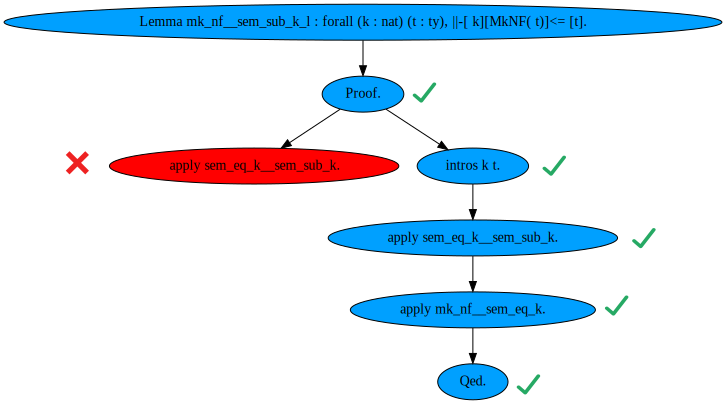
\includegraphics[width=0.70\textwidth]{maintenance/fig/example-graph.png}
  \caption{An example search tree, generated from the collected data
    by \toolname. It shows the user attempting to apply a lemma, which
    fails until they first run the \lstinline{intros} tactic.}
  \label{fig:search-tree}
\end{figure*}

\Cref{fig:tactics-table} shows the counts for each tactic
(regardless of arguments) in the 70 successful interactive proof subsessions.
%From this table, we can see that the
The distribution of tactics run was top-heavy; over 50\% of the tactics
invoked were either \lstinline{apply}, \lstinline{intros},
\lstinline{destruct}, \lstinline{rewrite}, \lstinline{exists}, \
\lstinline{unfold}, or \lstinline{simpl}.
The \lstinline{apply} tactic had a significant lead over other tactics
in invocations, but invocations of \lstinline{destruct} ended in
failure or stepping above them nearly as many times as invocations
of \lstinline{apply} did.

This data indicates two takeaways for proof tooling:
Firstly,
\begin{displayquote}
  \textbf{Takeaway:}
  Tools may be able to focus on understanding the behavior of
  and suggesting just a small number of tactics,
  and still benefit.
\end{displayquote}
And second, since lemma and hypothesis application was the main driver of proofs,
\begin{displayquote}
  \textbf{Takeaway:}
  Assessing which lemmas and hypotheses are useful would be one of the main tasks of
  a tool which suggests tactics to the user.
\end{displayquote}
The machine learning tool ML4PG~\cite{Komendantskaya2012} for Coq
already offers promising developments in this direction by understanding
and providing hints about similar lemmas,
as does the proof automation tool CoqHammer~\cite{coqhammer};
similar functionality may help
improve the performance of tools that suggest tactics.

\subsection{Fixing Proofs by Fixing Tactics}
\label{sec:fixes}

%While the raw cancellation numbers are useful, they do not give a
The raw cancellation numbers do not give a
broader context to each cancellation, namely what tactic it was
cancelled in favor of. To address this, we built a search
graph and analyzed the tactic attempts at each branching node (see
\Cref{fig:search-tree}). Where there were more than 2 attempts, we
compared all non-final attempts to the final one separately.

In our 71 successful interactive proof subsessions, 96 tactics
were cancelled in favor of another tactic at the same state.
Of the 96 cancelled-tactic and final-tactic pairs: %, we found:
\begin{itemize}
\item 13 were semicolon clauses added after a tactic, like:
  \begin{lstlisting}
    destruct w. $\to$ destruct w; reflexivity.
  \end{lstlisting}
\item 4 were semicolon clauses removed from the end of a tactic, like:
  \begin{lstlisting}
    intros; reflexivity. $\to$ intros.
  \end{lstlisting}
\item 31 were the same tactic with modified arguments, like:
  \begin{lstlisting}
    intros k X t. $\to$ intros k X t Hfresh.
  \end{lstlisting}
\item 5 were similar, but a \lstinline{Search} or \lstinline{Check} command was first run
  before replacing the tactic, like:
  \begin{lstlisting}
    apply IdSetFacts.remove_3. $\to$ 
    Check IdSetFacts.remove_3. 
    apply IdSetFacts.remove_3 with Y.
  \end{lstlisting}
\item 43 changes did not fall into this categorization.
\end{itemize}

The proofs shown were complex, and users often made nontrivial
changes to attempted tactics, so not all changes could be
easily categorized or analyzed. However, over half of the changes
present could be categorized into simple changes, and potentially
synthesized by automated tools.

This data also shows us that for a large proportion of tactics, users
could correctly pick the tactic to invoke, even when they made
mistakes in its arguments. In addition, fixing these arguments took both
on average and in the worst case longer than fixing other kinds
of mistakes. Accordingly,
\begin{displayquote}
  \textbf{Takeaway:}
  Automated tooling that suggests actions to take
  based on tactics that were recently stepped above or failed
  may focus on predicting new arguments for the attempted tactic.
\end{displayquote}

\section{Q2: Changes to Terms}
\label{sec:q2}

Q2 asked what kinds of changes proof
engineers make to programs and specifications, and whether those
changes reveal patterns amenable to automation.
This information may be useful to ensure tools for proof evolution
support the features that help proof engineers.

\paragraph{A2}
We found that while no single change was dominant across
all users, users made related changes within and across sessions.
Analysis of these changes revealed four patterns:

\begin{enumerate}
\item Incremental development of inductive types
\item Repetitive refactoring of identifiers
\item Repetitive repair of specifications
\item Interactive discovery of programs and specifications
\end{enumerate}

\paragraph{Methodology}
To answer this question, we wrote a script to visualize changes over 
time as diffs on Github (see Figure~\ref{fig:ex-diff}).
The script reconstructed the state of the file up to 
each cancellation within a session, then committed that to the 
public data repository.
When possible (see Section~\ref{sec:wish2}), it augmented
each commit with information on whether the cancellation was a failure
or the user stepping up in an IDE.

We then manually analyzed the diffs that this visualization produced to 
build a classification of changes (Section~\ref{sec:class}), 
then classify changes that we found (Section~\ref{sec:changes}).
We did this for each of the 362 interactive sessions and, when relevant,
across sessions as well.
Finally, we looked at clusters of common changes for patterns.
For each of the four patterns we found
(Sections~\ref{sec:pat1},~\ref{sec:pat2},~\ref{sec:pat3}, and~\ref{sec:pat4}),
we identified benchmarks (examples of the pattern in our data)
and lessons for automation.

\subsection{Building a Classification}
\label{sec:class}

After running the visualization script, we did a manual analysis of the diffs
in order to build a classification of changes to Gallina terms.
This analysis was thorough in that it involved inspecting each
consecutive diff and, when relevant, diffs that spanned several commits
(when a user stepped up, changed something, and then later stepped back down)
or sessions (when a user modified the same file during two different sessions).
However, it did not necessarily capture all changes to terms;
Section~\ref{sec:wish2} discusses some of the challenges.

\paragraph{Classification}

We designed a classification that groups changes along three dimensions:

\begin{enumerate}
\item \textbf{Command}: vernacular command used to define the term in
                        which a subterm changed
\item \textbf{Operation}: how the subterm changed
\item \textbf{Location}: innermost subterm that changed
\end{enumerate}
with the following categories for \textbf{Operation}:

\begin{enumerate}
\item \textbf{Structure}:
\begin{enumerate}
\item \textbf{Add} or \textbf{Del}: add or delete information
\item \textbf{Mov}: move information
\end{enumerate}
\item \textbf{Content}:
\begin{enumerate}
\item \textbf{Pch} or \textbf{Uch}: patch or unpatch
\item \textbf{Cut} or \textbf{Uut}: cut or uncut
\item \textbf{Rpl}: replace
\end{enumerate}
\item \textbf{Syntax}:
\begin{enumerate}
\item \textbf{Rnm}: rename
\item \textbf{Qfy} or \textbf{Ufy}: qualify or unqualify
\end{enumerate}
\end{enumerate}
Changes listed together are inverse operations.
The \textbf{Structure} changes are straightforward.
Among the changes to \textbf{Content}, \textbf{Pch} is applying a function
to the old term to get a new term, \textbf{Cut} is defining a new term
or let-binding and then referring to that term inside of an existing term,
and \textbf{Rpl} is replacing contents in any other way.
Among the \textbf{Syntax} changes, \textbf{Qfy} is
qualifying a constant after changing an import.

For \textbf{Structure} changes, there are five \textbf{Location}s:

\begin{enumerate}
\item \textbf{Hyp}: hypothesis of anything that can take arguments
\item \textbf{Arg}: argument in an application
\item \textbf{Ctr}: constructor of an inductive type
\item \textbf{Cas}: case of a match statement
\item \textbf{Bod}: body of anything that can take arguments
\end{enumerate}

For \textbf{Content} changes, there are an additional two:

\begin{enumerate}
\setcounter{enumi}{5}
\item \textbf{Fun}: function in an application
\item \textbf{Typ}: type annotation
\end{enumerate}

For \textbf{Syntax} changes, there are only three:

\begin{enumerate}
\item \textbf{Bnd}: binding in the local environment
\item \textbf{Idn}: identifier in the global environment
\item \textbf{Con}: constant
\end{enumerate}

\paragraph{Design Considerations}

That classification that we designed considers changes only within
Gallina terms defined or stated using vernacular commands.
Since it is focused solely on changes to defined terms,
it does not consider other information like changes to vernacular commands,
hints, tactics, notations, scope annotations, inference information, or imports,
and it considers additions of new terms only in \textbf{Cut} changes.

In building this classification, we aimed to group
changes at a level of granularity narrow enough to inform the design of proof
engineering tools, but broad enough to capture patterns.
We suspect that within these categories, there are more granular
categories that can be useful for automation, like distinguishing among
hypotheses to set apart indices of inductive types, or classifying
a \textbf{Content} change as semantics-preserving.
We did not design a more granular classification because we did not
find it useful for describing our data.
%(we found no changes to indices of inductive types, for example).

\subsection{Classifying Changes}
\label{sec:changes}

Once we had designed this classification,
we used it to classify the changes that we had found.
We ignored intermediate changes that immediately failed to lex, parse, or type check.

\begin{figure*}
\small
\begin{tabular}{ |l|rrrr|l|l|l| }
\hline
     \textbf{User} &
     \multicolumn{4}{c|}{\textbf{Top Changes}} &
     \textbf{\# Changes} &
     \textbf{\# Interactive} &
     \textbf{Expertise}
\\
\hline
     \textbf{1} &
     \indpat{\textbf{Add} \textbf{Ctr} (23)} &
     \indpat{\textbf{Add} \textbf{Cas} (22)} &
     \refactorpat{\textbf{Qfy} \textbf{Con} \phantom{0}(6)} &
     &
     \phantom{0}69 &
     \phantom{0}10 &
     $\circ$ $\circ$ $\circ$
\\
%\hline
     \textbf{2} &
     \indpat{\textbf{Add} \textbf{Cas} \phantom{0}(4)} &
     &
     &
     &
     \phantom{0}10 &
     \phantom{00}3 &
     $\circ$ $\circ$ $\circ$ $\circ$
\\
%\hline
     \textbf{3} &
     \repairpat{\textbf{Pch} \textbf{Arg} (13)} &
     \pddpat{\textbf{Mov} \textbf{Arg} \phantom{0}(8)} &
     \textbf{Add} \textbf{Bod} \phantom{0}(7) &
     \textbf{Cut} \textbf{Arg} \phantom{0}(7) &
     \phantom{0}55 &
     101 &
     $\circ$ $\circ$ $\circ$ $\circ$ $\circ$
\\
%\hline
     \textbf{5} &
     \indpat{\textbf{Add} \textbf{Cas} (20)} &
     \indpat{\textbf{Add} \textbf{Ctr} (13)} &
     \indpat{\textbf{Add} \textbf{Hyp} (12)} &
     &
     \phantom{0}75 &
     \phantom{0}15 &
     $\circ$ $\circ$ $\circ$
\\
%\hline
     \textbf{7} &
     \refactorpat{\textbf{Rnm} \textbf{Idn} (42)} &
     \pddpat{\textbf{Mov} \textbf{Hyp} (18)} &
     \pddpat{\textbf{Add} \textbf{Hyp} (18)} &
     &
     151 &
     183 &
     $\circ$ $\circ$ $\circ$ $\circ$
\\
%\hline
     \textbf{8} &
     \repairpat{\textbf{Rpl} \textbf{Fun} (29)} &
     \pddpat{\textbf{Del} \textbf{Hyp} \phantom{0}(4)} &
     \pddpat{\textbf{Uch} \textbf{Arg} \phantom{0}(4)} &
     &
     \phantom{0}44 &
     \phantom{0}27 &
     $\circ$ $\circ$ $\circ$ $\circ$ $\circ$
\\
%\hline
     \textbf{10} &
     \pddpat{\textbf{Pch} \textbf{Arg} \phantom{0}(4)} &
     \textbf{Rpl} \textbf{Cas} \phantom{0}(3) &
     &
     &
     \phantom{0}15 &
     \phantom{0}15 &
     $\circ$ $\circ$ $\circ$
\\
%\hline
     \textbf{11} &
     \textbf{Pch} \textbf{Cas} \phantom{0}(3) &
     &
     &
     &
     \phantom{00}7 &
     \phantom{00}8 &
     $\circ$ $\circ$ $\circ$
\\
\hline
\end{tabular}
\caption{Top changes, by user.}
\label{tab:userchanges}
\end{figure*}
% TODO Talia: Check patterns in anything not highlighted
% TODO Talia: Check timestamps and integrate if interesting
% TODO!!! Check user 2 for some constructors.

\begin{figure*}
\begin{minipage}{0.41\textwidth}
\centering
\includegraphics[width=0.7\textwidth]{maintenance/fig/diffs1.png}
\end{minipage}
\hfill
\begin{minipage}{0.57\textwidth}
\centering
\includegraphics[width=0.7\textwidth]{maintenance/fig/diffs2.png}
\end{minipage}
\caption{A change to an inductive type (left) and corresponding change to a fixpoint (right) that User 5 made in Session 19.}
\label{fig:ex-diff}
\end{figure*}

Classifying changes revealed clusters of related changes.
Further inspection of those clusters revealed common development patterns.
Figure~\ref{tab:userchanges} lists, for each user, the top three changes
by \textbf{Operation} and \textbf{Location} 
(four if there was a tie, and ignoring changes that we found fewer than three times for the user),
the total number of changes that we found,
and the total number of  interactive sessions and self-rated expertise
for reference.
Changes for which more detailed inspection revealed patterns
are highlighted in corresponding colors:
\indpatt{blue} for incremental development,
\refactorpatt{orange} for refactoring, \repairpatt{pink} for
repair, and \pddpatt{grey} for discovery.

The remainder of this section discusses these patterns, complete
with an example, benchmarks, and lessons for automation 
for each.
The benchmarks and lessons for automation are mainly for tool designers:
The benchmarks point to changes in specific sessions, the partial or 
complete automation of which would have helped our users.
The lessons for automation are natural directions for improvements
to proof engineering tools given the patterns we have observed.

The public data repository contains a complete list of the changes
that we classified, as well as a detailed walkthrough of each benchmark.

\subsubsection{Incremental Development of Inductive Types}
\label{sec:pat1}

The most common changes for Users 1 and 5 were adding cases to match statements
(\textbf{Add} \textbf{Cas}) and adding constructors to inductive types
(\textbf{Add} \textbf{Ctr}).
These changes corresponded to incremental development of inductive types,
followed by corresponding extensions to match statements of functions
that destruct over them, or to inductive types that depend
on or relate to them.
This pattern sometimes spanned multiple sessions.
While this pattern was most prevalent for Users 1 and 5, it was also
present for Users 2 and 7.

The diffs in Figure~\ref{fig:ex-diff} show an example change to
an inductive type, along with a corresponding change to a fixpoint.
The change on the left adds five constructors and moves one constructor down.
The change on the right adds five corresponding cases and moves one
corresponding case down.

\paragraph{Benchmark 1}

The example change from \Cref{fig:ex-diff} came from
User 5, Sessions 18, 19, 27, 33, and 35.
There, over the course of three weeks, the user incrementally developed the inductive type \lstinline{Term}
along with a record \lstinline{EpsilonLogic} and fixpoints
\lstinline{simplify} (later renamed to \lstinline{identity}) and \lstinline{free_vars}.

\paragraph{Benchmark 2}

In Sessions 37 and 41, over two days,
User 1 incrementally developed similar inductive types
\lstinline{ST} and \lstinline{GT}, as well as fixpoints
\lstinline{Gamma}, \lstinline{Alpha}, and \lstinline{eq} 
that referred to them.

\paragraph{Lessons for Automation}

Given that several users show this pattern,
this is one use case for which better automation may help.
Automation may help proof engineers adapt other inductive types,
match statements, and proofs after extending inductive types
with new constructors.
We are not aware of any work on adapting related inductive types and 
match statements.
There is some work on adapting proof obligations to new
constructors~\cite{Boite2004},
and a proposed algorithm for generating proofs that satisfy those
obligations~\cite{Mulhern06proofweaving}, but nothing that exists for
a current version of Coq.

\begin{displayquote}
  \textbf{Takeaway}:
  Proof engineers could benefit from automation to help update proofs and definitions
  after adding constructors to inductive types.
  %% Up-to-date automation to help proof engineers adapt definitions
  %% and proofs after extending inductive types is an unaddressed
  %% opportunity make an impact.
\end{displayquote}

\subsubsection{Repetitive Refactoring of Identifiers}
\label{sec:pat2}

Users 1 and 7 showed a pattern of repetitive refactoring, through
qualifying constants after changing imports (\textbf{Qfy} \textbf{Con}),
and renaming identifiers (\textbf{Rnm} \textbf{Idn}) and the constants
that referred to them (\textbf{Rnm} \textbf{Con}), respectively.
This pattern sometimes spanned multiple sessions, and even simple refactorings
sometimes resulted in failures.

Figure~\ref{fig:refactor} shows an example renaming from the five
definitions at the top to the five definitions at the bottom.
The change renames the identifiers of these definitions to
follow the same convention, then makes the corresponding changes
to constants in the bodies of the last two definitions.  

\begin{figure}
  \includegraphics[width=0.19\textwidth]{maintenance/fig/refactor.png}
  \caption{Renaming of definitions in User 7, Session 93.}
  \label{fig:refactor}
\end{figure}

\paragraph{Benchmark 3}

The example from \Cref{fig:refactor} came from User 7, Session 93.
The definition of \lstinline{ty} failed, since User 7 had already
defined an inductive type with that name.
In response, User 7 renamed all of these
to follow the same convention.
This took four attempts, but only a few minutes.

\paragraph{Benchmark 4}

In Session 193, User 7 split the \lstinline{TVar} constructor
of the inductive type \lstinline{ty} into two constructors:
\lstinline{TBVar} and \lstinline{TFVar}. User 7 at the same time
split the fixpoint \lstinline{FV} into \lstinline{FFV} and
\lstinline{FBV}.
In Session 198, User 7 at the same time renamed the broken lemma
\lstinline{b_subst_var_eq} to \lstinline{b_subst_bvar_eq},
and substituted in \lstinline{TBVar} for \lstinline{TVar} in its body.

\paragraph{Benchmark 5}

User 1 imported the \lstinline{List} module in Session 37, commit 10.
After the import, \lstinline{In} referred to the list
membership predicate from the standard library, whereas previously it had
referred to \lstinline{Ensembles.In}. The 6 qualify constant changes that we
found for User 1 were changing \lstinline{In} to \lstinline{Ensembles.In}
inside of three existing definitions.
This took multiple tries per definition,
but only a few minutes in total.

\paragraph{Lessons for Automation}

Refactoring terms (rather than proof scripts) as in
RefactorAgda~\cite{wibergh2019} and Chick~\cite{robert2018}
would have helped our users, but few refactoring tools for
ITPs support this~\cite{PGL-045}, and neither of these are implemented
for Coq.
Supporting making similar changes throughout a program, like Chick does,
may be especially useful.
Semantics-aware refactoring support may take this even further:
A refactoring tool for Coq may, for example, determine that an import
shadows an identifier, compute what the identifier used to refer to,
and refactor appropriately.
Or, it may guide the user to rename terms that refer to other
recently renamed terms.
Both of these would have helped our users.

\begin{displayquote}
  \textbf{Takeaway}:
  Refactoring and renaming tools,
  similar to those available for programmers in languages like Java,
  could also help proof engineers,
  and could potentially be more powerful in ITPs.
%%   Proof refactoring tools should support term refactoring,
%% especially patterns of term refactoring that are informed by Coq's semantics.
\end{displayquote}

\iffalse
Hooking into the REPL, like \toolname does, may help refactoring tools
make these suggestions independently of the UI.
\fi

\subsubsection{Repetitive Repair of Specifications}
\label{sec:pat3}

The top changes that we found for Users 3 and 8 were 
patching arguments (\textbf{Pch} \textbf{Arg}) and replacing functions
(\textbf{Rpl} \textbf{Fun}), respectively.
These corresponded to a pattern of repetitive repair of specifications,
often over several sessions.
Sometimes these repairs were necessary in order for the specification to
type check or for existing tactics to succeed.
Sometimes, after repairing specifications, users also repaired their proofs.

\begin{figure}
  \includegraphics[width=0.47\textwidth]{maintenance/fig/patch.png}
  \caption{Patches to a lemma in User 3, Session 73.}
  \label{fig:patch}
\end{figure}

Figure~\ref{fig:patch} shows an example change patching the arguments
of a lemma. This change wraps two arguments into a single application
in three different hypotheses of a lemma.

\paragraph{Benchmark 6}

11 of the 13 patches to arguments that we found for User 3,
including the example in \Cref{fig:patch}, came from Session 73.
All of these changes similarly wrapped arguments into an application of
\lstinline{Val}.
We suspect that this was due to a change in the definition of \lstinline{absr},
but we were not able to confirm this since
the change in question occurred before the beginning of the study.
The user admitted or aborted the proofs of four of the five
changed lemmas.

\iffalse
For the same reason, we were not able to determine with certainty
that the changes to proofs in that session were corresponding
repairs to match the new specification.
\fi

\paragraph{Benchmark 7}

28 of the 29 replace function changes that we found for User 8
were changes from \lstinline{=} to \lstinline{==} over
the course of about a week in Sessions
2, 14, 37, 40, 65, 79, 108, 125, and 160.
The corresponding proof attempts suggest that while these terms were well-founded with \lstinline{=}, the changes to use \lstinline{==}
may have been necessary to make progress in proofs
using certain tactics.
Sometimes, after making these changes, User 8 also fixed tactics
that had worked before.

\paragraph{Lessons for Automation}

Automation may help with these sorts of repairs to theorems
and proofs. The proof repair tool \textsc{PUMPKIN PATCH} already handles some
repairs to proofs after changes to both
\textbf{Content}~\cite{Ringer2018} and \textbf{Structure}~\cite{Ringer2019}, but has support for repairing the theorem statement itself only in
the latter case, and only for a specific class of changes to inductive types.
These changes provide examples where changing the theorem type is also
desirable, and may make good benchmarks for further development
to support this.

\begin{displayquote}
  \textbf{Takeaway}:
  Proof repair tools should repair programs and specifications,
  not just proofs.
\end{displayquote}

\subsubsection{Interactive Discovery of Programs and Specifications}
\label{sec:pat4}

In Q1 (Section~\ref{sec:q1}), we found that users most often fixed
proofs by stepping up outside of proofs and changing other things.
Our observations from Q2 are consistent with this,
and give some insight into the details.
Changes from Users 3, 7, 8, and 10 all revealed a pattern of interactive
discovery of programs and specifications:
In some cases, these users discovered bugs in their programs during a
proof attempt or test.
In other cases, these users discovered that their specifications were
incorrect, too weak, or difficult to work with.
Users sometimes assigned temporary names to lemmas or theorems,
then renamed them only after finalizing their types.
Even experts made mistakes in programs and theorem statements
(perhaps they were the ones catching them most effectively).

\begin{figure}
  \includegraphics[width=0.35\textwidth]{maintenance/fig/bad.png}
  \caption{A partial attempt at proving and later correction to an incorrect theorem from User 3, Session 11377 (tactic formatting is not preserved in the data
that \toolname receives).}
  \label{fig:bad}
\end{figure}

Figure~\ref{fig:bad} shows an example of catching a bug in a specification
during an attempted proof attempt. The theorem
before the change is impossible (let \lstinline{m} be \lstinline{3} 
and \lstinline{n} be \lstinline{1}).
After attempting to prove it and reaching this goal:

\begin{lstlisting}
  m : nat
  --------
  0 = m
\end{lstlisting}
the user steps up and fixes the theorem statement by replacing an argument
(\textbf{Rpl} \textbf{Arg}), then later finishes the proof.

\paragraph{Benchmark 8}

The change from \Cref{fig:bad} can be found in User 3, Session 11377.
The same session contains changes to the same theorem by
moving arguments (\textbf{Mov} \textbf{Arg}).
The user succeeded at the proof after about three minutes.
%All of the changes moving arguments that we found for User 3
%corresponded to interactive discovery of fixpoints and theorems.

\paragraph{Benchmark 9}

In Session 13, commit 11, User 10 patched a case (\textbf{Pch} \textbf{Cas})
of a fixpoint \lstinline{fib'} after testing.
This took the user about thirty seconds.
The fixpoint \lstinline{fib'} itself may have been used to 
test a different function.

\paragraph{Benchmark 10}

User 7 mainly demonstrated this pattern through
adding and moving hypotheses (\textbf{Add} and \textbf{Mov} \textbf{Hyp}).
The latter most often
corresponded to generalizing the inductive hypothesis 
after a partial proof attempt by swapping theorem hypotheses,
in some cases in order to induct over a different hypothesis 
altogether.
We found such changes in Sessions 19, 56, 93, 94, 104, 110,
153, 159, and 176.
See, for example, \lstinline{match_ty__value_type_l} in Session 94,
commit 15.

\paragraph{Benchmark 11}

In Session 2, User 7 temporarily named a lemma
\lstinline{weird_trans}, then renamed it to \lstinline{sub_r_nf__trans}
by Session 10 after finalizing its type after several partial
proof attempts over the course of about a day and a half.

\paragraph{Lessons for Automation}

The effect of discovering bugs by attempting a proof accounts for some
of the benefits of verification~\cite{murraybp}.
It makes sense, then, to continue to build automation to support users
in finding and fixing those bugs.
One possible unexplored avenue for this is integrating repair tools
with QuickChick~\cite{Paraskevopoulou2015} for testing specifications,
or with the \lstinline{induct} tactic from FRAP~\cite{FRAPBook}
or the hypothesis renaming functionality from CoqPIE~\cite{Roe2016}
for simple generalization of inductive hypotheses.
Integrating tools for discovering lemma and theorem names~\cite{Aspinall2016b}
during the development process may help users who use temporary names.
Above all, repair is not just something that happens to stable proof
developments---change is everywhere in developing those programs and
proofs to begin with.

\begin{displayquote}
  \textbf{Takeaway}: Integrating tools for proof repair with tools
  for discovery and development of specifications
  is an unaddressed opportunity to support proof engineers.
\end{displayquote}


%\section{Conclusions \& Future Work}
\label{sec:discussion}

We built \toolname, a Coq plugin that remotely collects fine-grained
proof development data in a way that is decoupled from the UI.
Using \toolname, we collected data on changes to proofs, programs,
and specifications at a level of granularity not previously
seen for an ITP.
Visualization and analysis of this data revealed evidence in our study
population of development patterns, at times confirming folk knowledge---like 
that discovering  the correct program or specification was often a
conversation with the proof itself, even for experts---and providing
useful insights and benchmarks for tools.

The infrastructure that we have built and the data that we have collected
using it are publicly available.
We hope to see it used as benchmarks for the improvement of
proof engineering tools, and as data for future studies.
We hope to see the infrastructure that we have built reused or
adapted to other ITPs for future studies.

\paragraph{Three Wishes}
We would like for our experiences building and using \toolname
to help the community conduct more studies of proof development processes.
We thus conclude with three wishes, the fulfillment of which would help
address the challenges that we encountered along the way:

\begin{enumerate}
\item Better abstraction of user environments (Section~\ref{sec:wish1})
\item More information about user interaction (Section~\ref{sec:wish2})
\item More users (Section~\ref{sec:wish3})
\end{enumerate}
We discuss how to grant each wish both at the level of study design
and at the level of ITP design in order to facilitate future studies of 
this kind.

\subsection{Wish: Better Abstraction of User Environments}
\label{sec:wish1}

In order to cast as broad of a net as possible for potential users, we
designed \toolname to be independent of the UI, 
the version of Coq, and the build system. Coq's plugin infrastructure
and interaction model offered a promising avenue for this,
%Together with the Coq developers, we were able to extend the plugin API
%with a hook to listen to Coq's REPL.
and Coq's resource file infrastructure meant that users could load the plugin
universally with just one LOC in one location.
All of this gave us the impression of independence from the details of
the UI, ITP version, and build system.

We later found that, while this infrastructure was useful,
the impression of total independence was somewhat of an illusion; 
all of these details mattered.
In particular, while \toolname itself was UI-independent, the analyses
that we ran did not achieve full independence.
For example, we found that depending on the version of Coq and what
event triggers a cancellation, different UIs use different mechanisms
for cancellation (recall these mechanisms from Section~\ref{sec:plugin}). 
Our analyses had to deal with all of these mechanisms.

In addition, partway through the study, we received a bug 
report that noted that one common build system for Coq compiles files by
default using a flag that disables loading the Coq resource file.
This is one possible explanation for the lack of data that some users sent.
To remedy this, we must ask future users of \toolname
to compile all of their Coq projects without using this flag;
we have updated the \toolname documentation to account for this. 

\paragraph{The Study Designer} Without help from the ITP designer,
the study designer cannot achieve full abstraction from these details.
The study designer may, however, work around the lack of full abstraction.
We recommend testing the study infrastructure with 
many different environments for many different scenarios.
It may help to identify potential users early and survey their
development environments before even beginning to test,
covering likely scenarios in advance.
It may also help to build in a short trial period on the final users
before the final data collection begins, thereby
covering their particular development environments.
The latter has the additional benefit of giving the study designer
time to discover and discuss with users possible confounding
variables for analysis, like development style or project phase.

We had the foresight to test \toolname with \lstinline{coqtop}, 
Proof General, and CoqIDE, but we did not anticipate User 5's custom
UI, which treated failures differently from the others.
We also did not anticipate the behavior of different
build systems on Coq's resource file, since we tested only one
build configuration.
We could have avoided both of these issues with our recommendations.
Instead, we had to work around both issues after deployment.

\paragraph{The ITP Designer} 
Most of the power to grant this wish is in the hands of the ITP designer.
Full abstraction over development environments may not be possible, but the
ITP designer may design the interaction model with this as a goal.
The REPL and state machine already strive for this---and come
close to achieving it---but their current implementations in Coq fall short.
Improvements to abstraction here may be minimal, like
providing fewer mechanisms for UIs to accomplish the same thing,
or providing a way to guarantee that a plugin is always loaded for all
build systems.

For a more radical approach, the ITP designer may look to other 
interaction models.
For example, Isabelle/HOL has recently moved away from its REPL,
instead favoring the Prover IDE (PIDE)~\cite{Wenzel2012} framework
as its interaction model.
With PIDE, UIs and ITPs communicate using an asynchronous protocol to manage
versions of a document~\cite{Wenzel2014}, annotating the document with 
new information when it becomes available~\cite{Wenzel2012}.
Personal communication suggests that there is an ongoing attempt to 
to centralize functionality like the build system into PIDE.
While centralization may limit the potential for customization by different
UIs, it may make studies of fine-grained proof development data easier,
since the instrumentation may occur at a higher level,
guaranteeing more uniform interaction.

\subsection{Wish: More Information about User Interaction}
\label{sec:wish2}

By observing state machine messages through the plugin API,
we were able to log data at high enough granularity to reconstruct
hundreds of interactive sessions. This helped us identify incremental
changes to tactics and terms that are difficult to gather from other sources.

The hooks that we designed together with the Coq developers, however, 
were not perfect.
There was no way for us to use those hooks to listen to the messages
that Coq sent back to the UI.
Making this change would have required modifying Coq again, and by the time
we realized this, it was too late.
Listening to those responses would have given us more insight into user
behavior.
It would have also helped us distinguish between failures and stepping up.
Instead, we had to distinguish between these using IDE-specific heuristics,
which left us with no automatic way to distinguish failures from stepping up
for User 5's custom UI.

We also found that once we had collected granular data, 
analyzing it was sometimes difficult. 
For example, sometimes users defined a term, stepped up and changed
an earlier term, then stepped back down and changed the original term.
For such a change, our visualization script constructed 3 consecutive commits;
to determine that the original term had changed, we had to look at 
the difference between the 1st and the 3rd commits.
Sometimes, changes occurred over tens of commits, or over several sessions.
Thus, manual analysis of changes for Q2 was tedious, and involved
not only inspecting thousands of diffs but also understanding each 
session well enough to track term information over time.

We considered automating the analysis for Q2, but we found
automatically classifying changes in terms to be prohibitively difficult.
While part of this was due to the inherent difficulty of the problem,
part of this was also due to missing information:
When the UI backed up to an earlier state, we did not know what was below 
the command or tactic corresponding to that state in the file. 
So, when a user copied and pasted a term and then modified both versions,
or made several changes at once to a term before stepping 
down below it, even manually deciding whether it was the same term 
that had changed or a new term entirely proved to be difficult.

\paragraph{The Study Designer}
To grant this wish, we recommend that the study designer run a beta test, complete with analysis, as we did---and that they do so early,
as we did not.
That way, there is enough time to address needs discovered during testing,
for example by communicating with ITP designers.
It may also help to use multiple methods for data collection,
for example by augmenting the collected data with information from the IDE
to track the state of definitions in the file below the location to
which the user has stepped.

The beta testing phase was extremely useful to us; as a result we
reworked our server infrastructure to receive and easily
analyze larger amounts of data, and we tested data backup
infrastructure and network failure resilience code. 
We also discovered and reported a 
bug\footnote{\url{http://github.com/coq/coq/issues/8989}} in CoqIDE and 
Proof General that had made it impossible for us to tell which 
sessions corresponded to which files; the fix was marked as critical 
and backported to Coq 8.9, so only the analyses for Users 5 (custom UI), 8 (Coq 8.8), and 10 (Coq 8.8) were impacted.
However, while we discovered the lack of response information in the plugin hooks
during this period, we did not have enough time to coordinate with Coq developers on
changes to the hooks. 
Leaving more time between testing and the final study would have helped us.

\paragraph{The ITP Designer} 
By implementing hooks like the one that we helped implement for Coq,
the ITP designer can make it easier for researchers to study 
proof development processes. 
To grant this wish, we recommend that these hooks expose not just 
request information, but also response information, 
especially error information.

Augmenting the interaction model with more information
about the file may also help.
For example,
the interaction model could expose a simple and uniform way for UIs
to track that a definition in a new state corresponds to a definition 
in a previous state (that is, that the user did not remove that
definition from the file and replace it with something entirely new). 
This could make it much simpler for an analysis to track changes to a definition over time,
and to choose the granularity with which to inspect changes.
There is some tension between this and the wish for abstraction from
Section~\ref{sec:wish1}, but it may be worth weighing the tradeoffs.

\subsection{Wish: More Users}
\label{sec:wish3}

We attempted to recruit a large and representative sample of Coq proof
engineers.
In our attempts to recruit users, we contacted programming
languages groups at several universities that were known to be working
with Coq, and emailed \lstinline{coq-club} with our project
pitch. We included a promotional video in the hopes of
attracting as many users as possible.

In the end, however, we were able to recruit only 12 users,
all of whom were intermediate through expert users with at least two years
of Coq experience. We received interactive sessions for just 8 of 12
of these users. While this data was rich and granular, with just 8 users,
we were not able to reach broad conclusions about proof engineers more generally.

Part of this was likely due to the demographics of the
community: Compared to other programming environments,
Coq has only a small number of users,
many of whom have or are pursuing graduate degrees.
However, part of this may have been due to
deterrents in our screening process, or poor incentives for our users.

\paragraph{The Study Designer}
The study designer may fulfill this in part by casting as broad of a net
as possible, carefully considering any deterrents in screening criteria.
It may help to use welcoming language to encourage potential users
who are unsure if they qualify.
To reach beginner users, it may help to recruit students.
To reach a more international audience, it may help to distribute
promotional materials and consent forms in multiple languages.
It may also help to consider incentives that appeal to proof engineers.
However, until the ITP user community grows significantly, it will continue 
to be difficult to conduct large-scale studies of proof engineering.

We reached users from different institutions, but
most of our users had similar levels of expertise. We suspect that this was
in part because we asked for users to have at least a year of 
experience using Coq, so as to avoid mixing in data from
users learning Coq for the first time.
We also required fluency in English to ensure that users understood
the consent forms.
Both of these may have deterred users.
One potential user who did not participate noted that we did not make
it clear in our recruitment materials that data from occasional rather
than frequent Coq users was still useful to us.
The same potential user noted that we could have engaged more
with community leaders, thereby giving others in the community
more incentive to participate.
We considered monetary incentives, but ultimately decided they were less
tempting to the community than appeals to improving tools.
Perhaps this was misguided or attracted a more advanced population,
and perhaps we could have considered a different incentive.

\paragraph{The ITP Designer}
The ITP designer may help reduce the costs of participating in these studies. 
We suspect that the primary gains here will come from continuing to 
break down barriers to using plugins and other outside tooling. 
Some examples of this include reducing the brittleness of plugin APIs 
over time, improving build and distribution systems, making it possible 
to prove that a plugin does not interact with a kernel in a way that 
could compromise soundness of the system, 
and providing more support for users who port proof developments
and tools between ITP versions.

Of course, continuing to improve the ITP itself may continue 
to expand the community to reach more users. 
This may cause a positive feedback loop, helping to collect more data 
in order to drive further improvements to the ITP, in turn continuing to help
the community grow.




%\section{Related Work}

Our work builds upon prior research in proof reuse, proof automation, proof engineering, refactoring, differencing \& incremental computation,
programming by example, and program repair.

\paragraph{Proof Reuse} Our approach reimagines the problem of proof reuse in the context of proof automation.
While we focus on changes that occur over time, traditional proof reuse techniques can help
improve our approach.
Existing work in proof reuse focuses on transferring proofs between isomorphisms,
either through extending the type system~\cite{Barthe:2001:TIP:646793.704711} or through an automatic method~\cite{Magaud2002}.
This is later generalized and implemented in Isabelle~\cite{Huffman2013} and Coq~\cite{zimmermann2015automatic, tabareau2017equivalences};
later methods can also handle implications. 
%Transfer tactics apply these functions but do not infer them, while our approach
%infers these functions but does not apply them.
Integrating a transfer tactic with a proof patch finding tool will create an end-to-end
tool that can both find patches and apply them automatically.

Proof reuse for extended inductive types~\cite{Boite2004} adapts proof obligations
to structural changes in inductive types. Later work~\cite{Mulhern06proofweaving} proposes a method
to generate proofs for new constructors. These approaches may be useful when extending the differencing
component to handle structural changes. Existing work in theorem reuse and proof generalization~\cite{Felty1994, pons00, Johnsen2004} abstracts existing proofs for reusability, and may be useful
for improving the abstraction component.
Our work focuses on the components critical to searching for patches; these complementary approaches
can drive improvements to the components.

\paragraph{Proof Automation} We address a missed opportunity in proof automation for ITP: searching
for patches that can fix broken proofs.
This is complementary to existing automation techniques. Nonetheless, there is a wealth
of work in proof automation that makes proofs more resilient to change. %; we discuss a sample.
Powerful tactics like \lstinline{crush}~\cite{chlipala:cpdt} can make
proofs more resilient to changes. 
Hammers like Isabelle's sledgehammer~\cite{Blanchette2013} can make proofs agnostic to some low-level changes.
Recent work~\cite{coqhammer} paves the way for a hammer in Coq.
%by translating a substantial subset of CIC into untyped
%first-order logic. 
Even the most powerful tactics cannot address all changes;
our hope is to open more possibilities for automation.

Powerful project-specific tactics~\cite{chlipala:cpdt, Chlipala2013} can help prevent low-level maintenance tasks.
Writing these tactics requires good engineering~\cite{Gonthier2011} and domain-specific knowledge,
and these tactics still sometimes break in the face of change.
%Furthermore, these tactics still sometimes break in the face of change. %, and when they do, they are difficult to debug.
A future patching tool may be able to repair tactics; the debugging process
for adapting a tactic is not too dissimilar to providing an example to a tool.

Rippling~\cite{rippling} is a technique for automating inductive proofs that uses restricted rewrite rules to
guide the inductive hypothesis toward the conclusion; this may guide improvements to the
differencing, abstraction, and specialization components.
The abstraction and factoring components address specific classes of unification problems;
recent developments to higher-order unification~\cite{Miller:2012:PHL:2331097} may help
improve these components.
Lean~\cite{selsam:lean} introduces the first congruence closure algorithm for dependent type theory that
relies only on the Uniqueness of Identity Proofs (UIP) axiom. While UIP is not fundamental to Coq,
it is frequently assumed as an axiom; when it is, it may be tractable to use a similar algorithm to improve the tool.

GALILEO~\cite{bundyreasoning} repairs faulty physics theories
in the context of a classical higher-order logic (HOL); there is preliminary work extending this
style of repair to mathematical proofs. 
Knowledge-sharing methods~\cite{tgck-cicm14} can adapt some proofs across different representations of HOL.
These complementary approaches may guide extensions to support decidable domains and classical logics.

\paragraph{Proof Engineering} Existing proof engineering work addresses brittleness
by planning for changes~\cite{proof-eng} and designing theorems and proofs that make maintenance less of an issue.
Design principles for specific domains (such as formal metatheory~\cite{Aydemir2008, Delaware2013POPL, Delaware2013ICFP})
can make verification more tractable. CertiKOS~\cite{certikos} introduces the idea of a deep specification to
ease verification of large systems.
Ornaments~\cite{Dagand17jfp, Williams:2014:OP:2633628.2633631}
separate the computational and logical components of a datatype, and may
make proofs more resilient to datatype changes.
These design principles and frameworks are complementary to our approach.
Even when programmers use informed design principles,
changes outside of the programmer's control can break proofs;
our approach addresses these changes.

There is a small body of work on change and dependency management for verification,
both to evaluate impact of potential changes and maximize reuse~\cite{873647, Autexier:2010:CMH:1986659.1986663}
and to optimize build performance~\cite{Celik:2017:IRP:3155562.3155588}.
These approaches may help isolate changes, which is necessary to identify future benchmarks, integrate
with CI systems, and fully support version updates.

\paragraph{Refactoring} Our approach is close in spirit to refactoring~\cite{Mens:2004:SSR:972215.972286}.
The Haskell refactoring tool HaRe~\cite{HaRe} automatically lifts definitions, and may be useful
for improving abstraction.
There is a growing body of work on refactoring in the context of ITP~\cite{Whiteside2011, Bourke_DKK_12}.
The IDE CoqPIE~\cite{Roe2016} and the verification platform Why3~\cite{Bobot2013} can
both adapt Coq proofs to simple syntactic changes.
It may be possible to use our lemma factoring component to improve proof refactoring tools.
Proof refactoring tools are semantics-preserving; unlike these tools,
our approach handles semantic changes.

\paragraph{Differencing \& Incremental Computation} Existing work in differencing and incremental computation may help 
improve our semantic differencing component.
Type-directed diffing~\cite{Miraldo:2017:TDS:3122975.3122976}
finds differences in algebraic data types.
Semantics-based change impact analysis~\cite{Autexier:2010:SCI:1860559.1860580} models semantic differences
between documents.
Differential assertion checking~\cite{differential-assertion-checking-2} analyzes different
versions of a program for relative correctness with respect to a specification.
Incremental $\lambda$-calculus~\cite{Cai:2014:TCH:2594291.2594304} introduces a general model for program changes.
All of these may be useful for improving semantic differencing.

\paragraph{Programming by Example} Our approach generalizes an example that the programmer provides.
This is similar to programming by example, a subfield of 
program synthesis~\cite{DBLP:journals/ftpl/GulwaniPS17}. 
This field addresses different challenges in different logics,
but may drive solutions to similar problems in a dependently typed language.

\paragraph{Program Repair} Adapting proofs to changes is essentially program repair
for dependently typed languages. 
Program repair tools for 
languages with non-dependent type 
systems~\cite{Pei:2014:APR:2731750.2731779, Long:2016:APG:2837614.2837617, Le:2017:SSS:3106237.3106309, Mechtaev:2016:ASM:2884781.2884807, Monperrus2015} 
may have applications in the context of a dependently typed language.
Similarly, our work may have applications within program repair in these languages:
Future applications of our approach may repurpose it to repair programs for functional languages.






\iffalse
(This subsection is not done yet, but not really needed to understand flow of paper.)

There are a lot of development processes people use to make proofs less likely to break to begin with (survey paper).

Two examples I like: First, affinity lemmas and reference to \lstinline{zip} example.
Second, better tactics like from CPDT and how could help is in \lstinline{zip} example.

Quick summary of some other ideas from survey paper.
For more, see the survey paper.

In that case, it may help us to define a more general \lstinline{patch} corresponding to the change:

\begin{lstlisting}
Lemma patch:
  forall {T$_1$} {T$_2$} (l$_1$ : list T$_1$) (l$_2$ : list T$_2$) (P : list (T$_1$ * T$_2$) $\rightarrow$ Type),
    length l$_1$ = length l$_2$ $\rightarrow$ 
    P (zip_same_length l$_1$ l$_2$) $\rightarrow$ 
    P (zip l$_1$ l$_2$).
Proof.
  intros. unfold zip.
  induction (eq_dec (length l$_1$) (length l$_2$)); simpl; auto.
  apply False_rect. auto.
Defined.
\end{lstlisting}
This says that it is possible to get between \textit{any} proof about \lstinline{zip_same_length}
and \textit{any} proof about \lstinline{zip}.
We can apply this in proofs about \lstinline{zip}:

\begin{lstlisting}
Proof.
  (@\codediff{intros. apply patch; auto.}@)
  (@\codediff{revert H. revert l$_2$.}@)
  induction l$_1$ as [|t$_1$ tl$_1$ IHtl$_1$].
  - auto.
  - intros l$_2$. induction l$_2$ as [|t$_2$ tl$_2$ IHtl$_2$].
    + intros H. auto.
    + intros H. simpl. rewrite IHtl1; auto.
Defined.
\end{lstlisting}
In Section~\ref{TODO}, I will show how \sysname can automatically extract patches like \lstinline{patch} % TODO would be great if it worked for this example
from example changes in proofs.
\fi



\section{Proof Repair}
\label{sec:mot-rep}

\kl{Proof repair} is a new form of \kl{proof automation} that automatically fixes broken proofs in response to change.
Unlike traditional proof automation, proof repair views programs, specifications, and proofs as fluid entities.
When a program or specification changes and this breaks proofs, proof repair extracts information from those
changes, generalizes it, and applies it to fix proofs broken by the change.

The name of proof repair is inspired by program repair~\cite{Monperrus:2018:ASR:3177787.3105906, Gazzola:2018:ASR:3180155.3182526},
or automatically fixing bugs in programs.
But my proof repair tools work differently from program repair tools, 
using a combination of \kl{semantic differencing} algorithms and \kl{proof term transformations} (Section~\ref{sec:how}).
All of this happens over low-level proof terms in \kl{Gallina}---and this is the key to success (Section~\ref{sec:infocert}).

\subsection{How Proof Repair Works}
\label{sec:how}

Recall my \kl{thesis}:

\begin{quote}
Changes in programs, specifications, and proofs can carry information that a tool can extract, generalize, and apply to fix other proofs broken by the same change. A tool that automates this can save work for proof engineers relative to reference manual repairs in practical use cases.
\end{quote}
My proof repair tools are the tools that automate this,
using a combination of semantic differencing and proof term transformations.
The \kl{differencing} algorithms compare the old and new version of the program, specification, or proof that has changed,
and from that extract the information carried by the change.
The \kl{transformations} then generalize that information and, in some cases, apply it to fix other proofs broken by the same change.
The details of all of this vary by the kind of breaking change,
as I will demonstrate in Chapters~\ref{ch:example} and~\ref{chapt:pi}.

% TODO an example would be nice here

The way that this works is quite different from the way that program repair tools typically work.
A number of program repair tools work by running tests or the programs themselves,
and many use fitness functions to identify candidate patches that 
are almost correct~\cite{Monperrus:2018:ASR:3177787.3105906}. % TODO check this
But there are not natural analogues of this in the world of proofs:
there are often no tests, it is not possible to just run the proof, and there is not a natural 
fitness function that describes what it means for a patch to a proof to be almost correct.

In addition, proof engineers write proofs in this high-level language of \kl{tactics}, \kl{Ltac}.
Each of these tactics is really a search procedure for a \kl{proof term}, so it is not straightforward to apply
typical program repair techniques to identify the next search procedure when a proof breaks.
Instead, proof repair tools can look down at the low-level language of proof terms, \kl{Gallina}.
But this is difficult: the type theory \kl{CIC$_{\omega}$} beneath Gallina is so rich that Gallina itself is quite unforgiving.
That is, even very small changes can produce proof terms that no longer type check.
But---and this is the key to proof repair---the unforgiving nature of Gallina actually turns out to be \textit{a good thing}.

\subsection{The Key to Proof Repair}
\label{sec:infocert}

The key to proof repair in this thesis is using the structure and information carried by Gallina proof terms.
In other words, differencing operates over Gallina terms,
and is guided by their semantics to narrow down the search space---it is \kl{semantic differencing}.
The transformations use the result of differencing to transform some proof term to a more general patch (in Chapter~\ref{ch:example})
or the patched proof itself (in Chapter~\ref{chapt:pi})---they are \kl{proof term transformations}.

This approach circumvents two of the biggest challenges in program repair:
gathering enough information to efficiently search for a patch,
and knowing when that patch is actually correct (Section~\ref{sec:repair}).
Thanks to the rich type theory beneath Gallina, changes in programs, specifications, and proofs
carry \textit{so much information} that my tools can use to search for a patch,
and proofs provide \textit{so much certainty} that the patch my tools find is correct in the end.
This is why proof repair works.

But this approach presents its own challenges,
like how to deal with the unforgiving nature of proof terms,
and how to produce friendly proof scripts in the end.
So Chapters~\ref{ch:example} and~\ref{chapt:pi} will show two tools that instantiate this approach,
and describe how these tools tackle these challenges.
Each chapter will introduce a tool that supports a different class of changes.
The first tool (Chapter~\ref{ch:example}) implements proof repair \kl{by example},
while the second tool (Chapter~\ref{chapt:pi}) implements proof repair \kl{across equivalences}.
Chapters~\ref{ch:example} and~\ref{chapt:pi} will follow a parallel structure:

\begin{itemize}
\item \textbf{Motivating Example} (Sections~\ref{sec:patch-motivating} and~\ref{sec:overview}):
an example that motivates the supported class of changes. 
\item \textbf{Approach} (Sections~\ref{sec:pumpkin-approach} and~\ref{sec:pi-approach}):
a high-level description of how the approach in Section~\ref{sec:how} is instantiated.
\item \textbf{Differencing} (Sections~\ref{sec:pumpkin-diff} and~\ref{sec:pi-diff}):
detailed explanations of the corresponding differencing algorithms.
\item \textbf{Transformations} (Sections~\ref{sec:pumpkin-trans} and~\ref{sec:pi-trans}):
detailed explanations of the corresponding proof term transformations.
\item \textbf{Implementation} (Sections~\ref{sec:pumpkin-impl} and~\ref{sec:pi-implementation}):
a description of the implementation of the approach as a tool for Coq.
\item \textbf{Results} (Sections~\ref{sec:pumpkin-results} and~\ref{sec:pi-results}):
results from case studies and experiments that show the tool can save work for proof engineers.
\item \textbf{Conclusion} (Sections~\ref{sec:pumpkin-concl} and~\ref{sec:pi-concl}):
a conclusion and reflection on how the thesis is validated so far.
\end{itemize}

Enjoy.

\paragraph{Historical Note}
Chapter~\ref{ch:example} draws on the 2018 work that introduced the original proof repair vision,
while Chapter~\ref{chapt:pi} draws on the more mature work that followed.
This difference in maturity permeates the \kl{results} of each chapter:

\begin{itemize}
\item \kl{Design}: Chapter~\ref{ch:example} describes its algorithms at a high level, as ad hoc heuristics
that sometimes struggle with undecidability.
It defines judgments for these algorithms as interfaces, but does not provide the derivations.
Chapter~\ref{chapt:pi} formalizes more elegant algorithms, building on insights from Chapter~\ref{ch:example},
and cleanly separating the decidable and undecidable parts.
\item \kl{Implementation}:
Chapter~\ref{ch:example} describes a \textit{prototype} plugin.
This prototype includes little automation for \textit{applying} patches,
integrates poorly into proof engineering workflows,
and does not properly unfold constants ($\delta$-reduce).
Chapter~\ref{chapt:pi} details technologies that address these limitations,
some of which can be used with the Chapter~\ref{ch:example} prototype if desired.
\item \kl{Case studies}:
Chapter~\ref{ch:example} shows only that a tool \textit{could have helped} proof engineers retroactively
on a few repair scenarios over small proofs of a fixed style.
Chapter~\ref{chapt:pi} shows that a tool
\textit{can help} and in fact \textit{has helped} proof engineers on a variety of real repair scenarios,
supporting larger proof developments (about 10000 LOC) in an order of seconds,
regardless of proof style.
\end{itemize}



\chapter{Often, Practically}

% TODO for now, just a copy-paste of DEVOID original paper, including the bib---will change soon, and add PLDI, and combine

\lstset{language=coq} % default

\section{Introduction}

%Proof assistants allow programmers to verify everything from distributed systems~\cite{wilcox:verdi} and compilers~\cite{leroy:compcert} to
%formalizations of mathematics~\cite{DBLP:journals/corr/BauerGLSSS16}. 

Proof automation makes verification more accessible to programmers, but it is often intractable
without programmer guidance. In \textit{interactive theorem proving} (ITP), the programmer guides the 
proof search process. The guidance reduces the search space to make proof automation more tractable.
This in turns helps the programmer, who does not have to manually verify the entire system.

%Interactive theorem provers allow programmers to guide proof search and interactively 
%verify everything from distributed systems~\cite{wilcox:verdi} and compilers~\cite{leroy:compcert} to
%formalizations of mathematics~\cite{DBLP:journals/corr/BauerGLSSS16}. In many of these theorem provers, programmers use

%In these languages, programmers write precise specifications of programs
%and prove implementations correct with respect to the specifications.

Despite automation, programming in these proof assistants is brittle: Even a minor change to a definition or theorem
can break many dependent proofs. This is a major source of development inefficiency in proof assistants
based on dependent type theory~\cite{proof-eng, Aydemir2008, Delaware2013ICFP}.

Traditional proof automation does not consider how proofs, definitions, and theorems change over time.
Instead, it is driven by the state of the current proof, sometimes with supplementary
information from other proofs, definitions, and theorems (as in hint databases~\cite{hints} and rippling~\cite{rippling}).
This puts the burden of dealing with brittleness on the programmer. 

We present a new approach to proof automation that accounts for breaking changes. %:
%searching the difference in versions of a proof, definition, or theorem. 
%We reimagine the problem of proof reuse~\cite{Boite2004, Mulhern06proofweaving} 
%in the context of traditional automation for ITP. 
In our approach, the programmer guides proof search 
by providing an \textit{example} of how to adapt proofs to changes in definitions or theorems.
A tool then generalizes the example adaptation into a \textit{reusable patch} that the programmer can use to fix
other broken proofs.

In doing so, we chart a path for a future %of ITP 
that moves the burden of brittleness
away from the programmer and into proof automation. 
Programmers typically address brittleness through design principles that make proofs
resilient to change~\cite{proof-eng, Aydemir2008, Delaware2013ICFP}, or through program-specific proof automation~\cite{chlipala:cpdt}.
These techniques, while useful, have limitations: 
Planning a verification effort around future change is challenging, and program-specific automation requires specialized knowledge.
The programmer's ability to anticipate likely changes determines the robustness of both techniques in
the face of change. %The robustness of both techniques in the face of change is determined by the programmer's ability to anticipate likely changes. 
Even then, many breaking changes are outside of the programmer's control. Updating proof assistant
versions, for example, can break proofs regardless of planning or automation~\cite{verdicommit}.

\begin{figure*}[ht]
\begin{minipage}{0.48\textwidth}
\centering
\lstset{language=coq, aboveskip=0pt, belowskip=0pt}
\lstinputlisting[firstline=1, lastline=3]{repair/izr.tex}
\lstinputlisting[backgroundcolor=\color{orange!35},firstline=4,lastline=5]{repair/izr.tex}
\lstinputlisting[firstline=6, lastline=6]{repair/izr.tex}
\end{minipage}
\hfill
\begin{minipage}{0.48\textwidth}
\centering
\lstset{language=coq, aboveskip=0pt, belowskip=0pt}
\lstinputlisting[firstline=8, lastline=10]{repair/izr.tex}
\lstinputlisting[backgroundcolor=\color{orange!35},firstline=11,lastline=12]{repair/izr.tex}
\lstinputlisting[firstline=13, lastline=13]{repair/izr.tex}
\end{minipage}
\vspace{-.3cm}
%\setlength{\belowcaptionskip}{-2pt}
\caption[Caption]{Old (left) and new (right) definitions of \lstinline{IZR} in Coq.
The old definition applies injection from naturals to reals and conversion of positives to
naturals; the new definition applies injection from positives to reals.}
\label{fig:izr}
\end{figure*}


We identify a set of core components that are critical to searching an example for patches in Coq.
We use the components to build %four different 
a procedure for finding patches %for non-structural changes 
in a Coq plugin as a 
proof-of-concept.
Case studies on real projects like CompCert~\cite{leroy:compcert} and the Coq standard library
suggest that patches are useful for realistic scenarios, and that it is simple to compose the components 
to handle different classes of changes.
We test the boundaries of the components on a suite of tests
and show how our findings can help build the future we envision.

In summary, we contribute the following:

\begin{enumerate}
%\item We develop new foundations for proof automation in ITP that account for breaking changes. % TODO reword
\item We identify a set of core components that are key to searching for patches.
\item We demonstrate that these core components are useful on real changes in Coq code.
\item We explore how to drive a future that moves the burden of change in ITP away from the programmer and into automated tooling.
\end{enumerate}

% TODO fix contributions

% evaluation stuff in contributions too

% SOMEWHERE: we focus on non-structural changes





\section{Motivating Example: Porting a Library}
\label{sec:example}

\toolnameb is a plugin for Coq 8.8; it can be found in the repository linked to as \textbf{Supplement Material} under the abstract of this paper.
To see how it works, consider an example using the types from Figure~\ref{fig:listvect},
the code for which is in \href{http://github.com/uwplse/ornamental-search/blob/itp+equiv/plugin/coq/examples/Example.v}{\lstinline{Example.v}}.
In this example, we lift two list zip functions and a proof of a theorem relating them from the Haskell CoreSpec library~\cite{hstocoqv}:
\begin{lstlisting}
zip {T$_1$ T$_2$}: list T$_1$ $\rightarrow$ list T$_2$ $\rightarrow$ list (T$_1$ * T$_2$).
zip_with {T$_1$ T$_2$ T$_3$} (f : T$_1$ $\rightarrow$ T$_2$ $\rightarrow$ T$_3$): list T$_1$ $\rightarrow$ list T$_2$ $\rightarrow$ list T$_3$.
zip_with_is_zip {T$_1$ T$_2$}: $\forall$(l$_1$:list T$_1$)(l$_2$:list T$_2$), zip_with pair l$_1$ l$_2$ = zip l$_1$ l$_2$.
\end{lstlisting}
\toolnameb runs a preprocessing step before lifting, which we describe in Section~\ref{sec:impl}; we assume this step has already run.
We use the \codeauto{cyan} background color to denote tool-produced terms and the names that refer to them.
We run \toolnameb to lift functions and proofs from lists to vectors, but it can also lift in the opposite direction.

\subparagraph*{Step 1: Search.}
We first use \toolnameb's \lstinline{Find ornament} command to search for the relation between lists and vectors:
\begin{lstlisting}
Find ornament list vector.
\end{lstlisting}
This produces functions which together form an equivalence (denoted \smallmath{$\simeq$}):
\begin{lstlisting}
list T $\simeq$ $\Sigma$ (n : nat).vector T n
\end{lstlisting}

\subparagraph*{Step 2: Lift.}
We then lift our functions and proofs
along that equivalence using \toolnameb's \lstinline{Lift} command.
For example, to lift \lstinline{zip}, we run the command:
\begin{lstlisting}
Lift list vector in zip as (@\codeauto{zipV\_p}@).
\end{lstlisting}
This produces a function with this type:
\begin{lstlisting}
(@\codeauto{zipV\_p}@) {T$_1$ T$_2$} : $\Sigma$ n.vector T$_1$ n $\rightarrow$ $\Sigma$ n.vector T$_2$ n $\rightarrow$ $\Sigma$ n.vector (T$_1$ * T$_2$) n.
\end{lstlisting}
that behaves like \lstinline{zip}, but whose body no longer refers to lists.
We lift our proof similarly:
\begin{lstlisting}
Lift list vector in zip_with_is_zip as (@\codeauto{zip\_with\_is\_zipV\_p}@).
\end{lstlisting}
This produces a proof of the analogous result (denoting projections by \smallmath{$\pi_{l}$} and \smallmath{$\pi_{r}$}):
\begin{lstlisting}
(@\codeauto{zip\_with\_is\_zipV\_p}@) {T$_1$ T$_2$} : $\forall$ (v$_1$ : $\Sigma$ n.vector T$_1$ n) (v$_2$ : $\Sigma$ n.vector T$_2$ n),
  (@\codeauto{zip\_withV\_p}@) pair ($\exists$ ($\pi_l$ v$_1$) ($\pi_r$ v$_1$)) ($\exists$ ($\pi_l$ v$_2$) ($\pi_r$ v$_2$)) =
  (@\codeauto{zipV\_p} ($\exists$ ($\pi_l$ v$_1$) ($\pi_r$ v$_1$)) ($\exists$ ($\pi_l$ v$_2$) ($\pi_r$ v$_2$)).
\end{lstlisting}
that no longer refers to lists, \lstinline{zip}, or \lstinline{zip_with} in any way.

\subparagraph*{Step 3: Unpack.}
The lifted terms operate over vectors whose lengths are \textit{packed} inside of a sigma type.
While this lets \lstinline{Lift} provide strong theoretical guarantees, it can make it difficult to interface with the lifted code.
We can recover \textit{unpacked} terms using \toolnameb's \lstinline{Unpack} command.
For example, to unpack \codeauto{\lstinline{zipV_p}}, we run the command:
\begin{lstlisting}
Unpack $\codeauto{zipV\_p}$ as $\codeauto{zipV}$.
\end{lstlisting}
This produces functions and proofs that operate directly over vectors, like \codeauto{\lstinline{zipV}}:
\begin{lstlisting}
(@\codeauto{zipV}@) {T$_1$ T$_2$} {n$_1$} (v$_1$ : vector T$_1$ n$_1$) {n$_2$} (v$_2$ : vector T$_2$ n$_2$) : 
  vector (T$_1$ * T$_2$) ($\pi_l$ ((@\codeauto{zipV\_p}@) ($\exists$ n$_1$ v$_1$) ($\exists$ n$_2$ v$_2$))).
\end{lstlisting}
and \codeauto{\lstinline{zip\_with\_is\_zipV}}:
\begin{lstlisting}
(@\codeauto{zip\_with\_is\_zipV}@) : $\forall$ {T$_1$ T$_2$} {n$_1$} (v$_1$ : vector T$_1$ n$_1$) {n$_2$} (v$_2$ : vector T$_2$ n$_2$),
  eq_dep _ _ _ ((@\codeauto{zip\_withV}@) pair v$_1$ v$_2$) _ ((@\codeauto{zipV}@) v$_1$ v$_2$).
\end{lstlisting}

\subparagraph*{Step 4: Interface.}
For any two inputs of the same length, \codeauto{\lstinline{zipV}} and \codeauto{\lstinline{zipV_with}} contain proofs
that the output has the same length as the inputs.
However, the types obscure this information.
\href{http://github.com/uwplse/ornamental-search/blob/itp+equiv/plugin/coq/examples/Example.v}{\lstinline{Example.v}} explains how to recover more user-friendly types, like that of \lstinline{zipV_uf}:
\begin{lstlisting}
zipV_uf {T$_1$ T$_2$} {n} : vector T$_1$ n $\rightarrow$ vector T$_2$ n $\rightarrow$ vector (T$_1$ * T$_2$) n.
\end{lstlisting}
and that of \lstinline{zip_withV_uf}:
\begin{lstlisting}
zip_withV_uf {T$_1$ T$_2$ T$_3$} (f : T$_1$ $\rightarrow$ T$_2$ $\rightarrow$ T$_3$) {n} : 
  vector T$_1$ n $\rightarrow$ vector T$_2$ n $\rightarrow$ vector T$_3$ n.
\end{lstlisting}
which both restrict input lengths.
We can then use our lifted functions and proofs in client code.
For example, we can write a different version of Coq's
\lstinline{BVand} function for bitvectors:
\begin{lstlisting}
BVand {n} (v$_1$ : vector bool n) (v$_2$ : vector bool n) : vector bool n := 
  zip_withV_uf andb v$_1$ v$_2$.
\end{lstlisting}
By working over lists, we are able to reason about only the interesting pieces, thinking about indices only
when relevant; in contrast, when writing proofs over vectors, even simple theorems
can generate tricky proof obligations.
With \toolnameb, the programmer can use the lifted functions and proofs
to interface with code that uses vectors, then switch back to lists when vectors are unmanageable. 
In essence, ornaments form the glue between these types.




\section{Specification}
\label{sec:spec}

This section specifies the two commands that \toolnameb implements:

\begin{enumerate}
\item \lstinline{Find ornament} searches for ornaments (specified in Section~\ref{sec:findspec}, described in Section~\ref{sec:findalg}).
\item \lstinline{Lift} lifts along those ornaments (specified in Section~\ref{sec:liftspec}, described in Section~\ref{sec:liftalg}). 
\end{enumerate}

\subparagraph*{Algebraic Ornaments.}
\toolnameb searches for and lifts along \textit{algebraic ornaments} in particular.
An algebraic ornament relates an inductive type \Aa\ to an indexed version of that type \B\ with a new index of type \IB,
where the new index is fully determined by a unique fold over \Aa. 
For example, \lstinline{vector} is exactly \lstinline{list} with a new index of type \lstinline{nat},
where the new index is fully determined by the \lstinline{length} function. Consequentially, there are two functions:
\begin{lstlisting}
ltv : list T $\phantom{blahblahblahblah}$ $\rightarrow$ $\Sigma$(n : nat).vector T n.
vtl : $\Sigma$(n : nat).vector T n $\rightarrow$ list T.
\end{lstlisting}
that are mutual inverses:
\begin{lstlisting}
$\forall$ (l : list T),$\phantom{blahblahblahblahb}$ vtl (ltv l) = l.
$\forall$ (v : $\Sigma$(n : nat).vector T n), ltv (vtl v) = v.
\end{lstlisting}
and therefore form the type equivalence from Section~\ref{sec:example}.
Moreover, since the new index is fully determined by \lstinline{length}, we can relate \lstinline{length} to \lstinline{ltv}:
\begin{lstlisting}
$\forall$ (l : list T), length l = $\pi_{l}$ (ltv l).
\end{lstlisting}

In general,
we can view an algebraic ornament as a type equivalence: % negative \vspace here is needed to deal with \vec{i}
\begin{lstlisting}
(@\vspace{-0.4cm}@)
$A\ \vec{i}\ \simeq\ \Sigma (n : I_B\ \vec{i}\phantom{_{,}}).B\ (\mathtt{index}\ n\ \vec{i}\phantom{_{,}})$
\end{lstlisting}
where \smallmath{$\vec{i}$} are the indices of \Aa, \IB\ is a function over those indices, 
and the \lstinline{index} operation inserts the new index \smallmath{$n$} at the right offset.
Such a type equivalence consists of two functions~\cite{univalent2013homotopy}:
\begin{lstlisting}
(@\vspace{-0.4cm}@)
promote : $A\ \vec{i}\ \phantom{blahblahblahblahblahbla_{,}} \rightarrow\ \Sigma (n : I_B\ \vec{i}\phantom{_{,}}).B\ (\mathtt{index}\ n\ \vec{i}\phantom{_{,}})$.
(@\vspace{-0.4cm}@)
forget$\phantom{e}$ : $\Sigma (n : I_B\ \vec{i}\phantom{_{,}}).B\ (\mathtt{index}\ n\ \vec{i}\phantom{_{,}})\ \rightarrow\ A\ \vec{i}$.
\end{lstlisting}
that are mutual inverses:\footnote{The adjunction condition follows from section and retraction.}
\begin{lstlisting}
(@\vspace{-0.4cm}@)
section$\phantom{ion}$ : $\forall\ (a : A\ \vec{i}\phantom{_{,}}),\ \phantom{blahblahblahblahblahbla_{,}} $forget$\ ($promote$\ a) \phantom{x} = a$.
(@\vspace{-0.4cm}@)
retraction : $\forall\ (b_{\Sigma} : \Sigma (n : I_B\ \vec{i}\phantom{_{,}}).B\ (\mathtt{index}\ n\ \vec{i}\phantom{_{,}})),\ $promote$\ ($forget$\ b_{\Sigma}) = b_{\Sigma}$.
\end{lstlisting}
An algebraic ornament is additionally equipped with an indexer, which is a unique fold:
\begin{lstlisting}
(@\vspace{-0.4cm}@)
indexer : $A\ \vec{i}\ \rightarrow\ I_B\ \vec{i}$.
\end{lstlisting}
which projects the promoted index:
\begin{lstlisting}
(@\vspace{-0.4cm}@)
coherence : $\forall (a : A\ \vec{i}\phantom{_{,}}),\ $indexer$\ a = \pi_{l}\ ($promote$\ a)$.
\end{lstlisting}
Following existing work~\cite{ko2016programming}, we call this equivalence the \textit{ornamental promotion isomorphism}; 
when it holds and the indexer exists, we say that \B\ is an algebraic ornament of \Aa.

\lstinline{Find ornament} searches for algebraic ornaments between types and is, to the best of our knowledge, the first search algorithm
for ornaments. \lstinline{Lift} then lifts functions and proofs along those ornaments, removing all references to the old type.
Both commands make some additional assumptions for simplicity; detailed explanations for these are
in \href{http://github.com/uwplse/ornamental-search/blob/itp+equiv/plugin/coq/examples/Assumptions.v}{\lstinline{Assumptions.v}}.

\subsection{\lstinline{Find ornament}}
\label{sec:findspec}

In their original form, ornaments are a programming mechanism: Given a type \Aa, an ornament determines
some new type \B. We invert this process for algebraic ornaments: Given types \Aa\ and \B, 
\toolnameb searches for an ornament between them. This is possible for algebraic ornaments precisely because the indexer is extensionally unique.
For example, all possible indexers for \lstinline{list} and \lstinline{vector} must compute
the length of a list; if we were to try doubling the length instead, we would not be able to satisfy the equivalence.

\lstinline{Find ornament} takes two inductive types and searches for the components of the 
ornamental promotion isomorphism between them:

\begin{itemize}
\item \textbf{Inputs}: Inductive types \Aa\ and \B, assuming:
\begin{itemize}
\item \B\ is an algebraic ornament of \Aa,
\item \B\ has the same number of constructors in the same order as \Aa,
\item \Aa\ and \B\ do not contain recursive references to themselves under products, and
\item for every recursive reference to \Aa\ in \Aa, there is exactly one new hypothesis in \B, which is exactly the new index of the corresponding recursive reference in \B.
\end{itemize}
\item \textbf{Outputs}: Functions \lstinline{promote}, \lstinline{forget}, and \lstinline{indexer}, guaranteeing:
\begin{itemize}
\item the outputs form the ornamental promotion isomorphism between the inputs.
\end{itemize}
\end{itemize}

\lstinline{Find ornament} includes an option to generate a proof that the outputs form the ornamental promotion isomorphism;
by default, this option is false, since \lstinline{Lift} does not need this proof.

\subsection{\lstinline{Lift}}
\label{sec:liftspec}

\lstinline{Lift} lifts a term along the ornamental promotion isomorphism between 
\Aa\ and \B. That is, it lifts types to corresponding types and terms of those types to corresponding terms:
\begin{lstlisting}
Lift list vector in list as $\codeauto{vector\_p}$. (* $\codeauto{vector\_p}$ T := $\Sigma$ (n : nat).vector T n *)
Lift list vector in (cons 5 nil) as $\codeauto{v\_p}$. (* $\codeauto{v\_p}$ := $\exists$ 1 (consV O 5 nilV) *)
\end{lstlisting}
Furthermore, it recursively preserves this equivalence, lifting non-dependent functions like \lstinline{zip}
so that they map equivalent inputs to equivalent outputs:
\begin{lstlisting}
$\forall$ {T$_1$ T$_2$} l$_1$ l$_2$, $\codeauto{promote}$ (zip l$_1$ l$_2$) = $\codeauto{zipV\_p}$ ($\codeauto{promote}$ l$_1$) ($\codeauto{promote}$ l$_2$).
\end{lstlisting}
This intuition breaks down with dependent types.
With equivalence alone, we can't state the relationship between \lstinline{zip_with_is_zip} 
and \codeauto{\lstinline{zip_with_is_zipV_p}}, since the unlifted conclusion:
\begin{lstlisting}
zip_with pair l$_1$ l$_2$ = zip l$_1$ l$_2$.
\end{lstlisting}
does not have the same type as the conclusion of the lifted version 
applied to promoted arguments; any relation between these terms must be heterogenous.

In particular, \lstinline{Lift} preserves the \textit{univalent parametric relation}~\cite{tabareau2017equivalences},
a heterogenous parametric relation that strengthens an existing parametric relation for dependent types~\cite{bernardy2012proofs}
to make it possible to state preservation of an equivalence:
Two terms \smallmath{$t$} and \smallmath{$t'$} are related by the univalent parametric relation 
\smallmath{$[[\Gamma]]_{u} \vdash [t]_{u} : [[T]]_{u}\ t\ t'$} at type \smallmath{$T$} in environment \smallmath{$\Gamma$}
if they are equivalent up to transport. The details of this relation can be found in the cited work.

\lstinline{Lift} preserves this relation using the components that \lstinline{Find ornament} discovers,
and additionally guarantees that the lifted term does not refer to the old type in any way:

\begin{itemize}
\item \textbf{Inputs}: The inputs to and outputs from \lstinline{Find ornament}, along with a term \smallmath{$t$}, assuming: %:
\begin{itemize}
\item the assumptions and guarantees from \lstinline{Find ornament} hold,
\item \IB\ is not \Aa,
\item \smallmath{$t$} is well-typed and fully \smallmath{$\eta$}-expanded,
\item \smallmath{$t$} does not apply \lstinline{promote} or \lstinline{forget}, and
\item \smallmath{$t$} does not reference \B.
\end{itemize}
\item \textbf{Outputs}: A term \smallmath{$t'$}, guaranteeing:
\begin{itemize}
\item if \smallmath{$t$} is \smallmath{$A\ \vec{i}$}, then \smallmath{$t'$} is \smallmath{$\Sigma (n : I_B\ \vec{i}\phantom{_{,}}).B\ (\mathtt{index}\ n\ \vec{i}\phantom{_{,}})$},
\item \smallmath{$t'$} does not reference \Aa, and
\item if in the current environment \smallmath{$\Gamma \vdash t : T$}, then \smallmath{$[[\Gamma]]_{u} \vdash [t]_{u} : [[T]]_{u}\ t\ t'$}.
\end{itemize}
\end{itemize}

\lstinline{Lift} does not require a proof
that the input components form the ornamental promotion isomorphism, but they must for the guarantees to hold. It can operate in either direction, promoting from \Aa\ to packed \B\ or forgetting in the opposite direction; the specification for the forgetful direction is similar, with extra
restrictions on how \B\ is used within \smallmath{$t$}.



\section{Algorithms}
\label{sec:alg}

This section describes the algorithms that implement the specifications
from Section~\ref{sec:spec}.

\subparagraph*{Presentation.} We present both algorithms relationally, using a set of judgments;
to turn these relations into algorithms, prioritize the rules by running the derivations in
order, falling back to the original term when no rules match.
The default rule for a list of terms is to run the derivation on each element of the list individually. 

\subparagraph*{Notes on Syntax.} The language the algorithms operate over is CIC$_{\omega}$ with primitive eliminators;
this is a simplified version of the type theory underlying Coq. Figure~\ref{fig:syntax}
contains the syntax (which includes variables, sorts, product types,
functions, inductive types, constructors, and eliminators),
as well as the syntax for some judgments and operations,
the rules for which are standard and thus omitted. 
For simplicity of presentation, we assume variables are names; 
we assume that all names are fresh.
As in Coq, we assume the existence of
an inductive type \sigT\ for sigma types with projections \Pil\ and \Pir;
for simplicity, we assume projections are primitive.
Throughout, we use \smallmath{$\vec{i}$} and \smallmath{$\{t_1, \ldots, t_n\}$} to denote
lists of terms, and we use \smallmath{$\vec{i}[j]$} to denote accessing the element of the list \smallmath{$\vec{i}$} at offset \smallmath{$j$}.

\subparagraph*{Common Definitions.}
The algorithms assume list insertion and removal functions \lstinline{insert} and \lstinline{remove},
plus two functions \toolnameb implements:
\lstinline{off} computes the offset of the new index of type \IB\ in \B's indices,
and \lstinline{new} determines whether a hypothesis in a case of the eliminator type of \B\ is new.
Figure~\ref{fig:common} contains other common definitions, the names for which are reserved:
The \lstinline{index} and \lstinline{deindex} functions insert an index into and remove an index from a list
at the index computed by \lstinline{off}.
Input type \Aa\ expands to an inductive type with indices % parameters and indices, really
of types \smallmath{$\vec{\mathrm{X}_A}$}, sort \smallmath{$\mathrm{s}_A$}, and constructors
\smallmath{$\{\mathrm{C}_{A_1}, \ldots, \mathrm{C}_{A_n}\}$}.
\smallmath{$\mathrm{P}_A$} denotes the type of the motive of the eliminator of \Aa,
and each \smallmath{$\mathrm{E}_{A_i}$} denotes the type of the eliminator for the $i$th constructor of \Aa.
Analogous names are also reserved for input type \B.

\begin{figure}
\begin{minipage}{0.52\textwidth}
\small
\begin{grammar}
<i> $\in \mathbbm{N}$, <v> $\in$ Vars, <s> $\in$ \{ Prop, Set, Type<i> \}

<t> ::= <v> | <s> | $\Pi$ (<v> : <t>) . <t> | \\
$\lambda$ (<v> : <t>) . <t> | <t> <t> | \\
Ind (<v> : <t>)\{<t>,\ldots,<t>\} | Constr (<i>, <t>) | \\
Elim(<t>, <t>)\{<t>,\ldots,<t>\}
\end{grammar}
\end{minipage}
\hfill
\begin{minipage}{0.48\textwidth}
\footnotesize
\begin{lstlisting}
$\Gamma$ $\vdash$ $t$ $:$ $T$ // type checking
$\Gamma$ $\vdash$ $t_1$ $\defeq$ $t_2$ // definitional equality
$t_\beta$ // beta-reduction
$t_{\beta\delta\iota}$ // normalization
$t$ $[y$ $/$ $x]$ // substitution
$\xi$ $(I,$ $Q,$ $c,$ $C)$ // type of eliminator
\end{lstlisting}
\end{minipage}
\vspace{-0.3cm}
\caption{CIC$_\omega$ syntax (left, from existing work~\cite{Timany2015FirstST}) and judgments and operations (right).}
\label{fig:syntax}
\end{figure}


\begin{figure}
\begin{minipage}{0.60\textwidth}
\begin{lstlisting}
(@\vspace{-0.4cm}@)
$A$ := $\mathrm{Ind} (\mathit{Ty}_A : \Pi (\vec{i_A} : \vec{\mathrm{X}_A}) . \mathrm{s}_A)\{\mathrm{C}_{A_1}, \ldots, \mathrm{C}_{A_n}\}$
(@\vspace{-0.4cm}@)
$B$ := $\mathrm{Ind} (\mathit{Ty}_B : \Pi (\vec{i_B} : \vec{\mathrm{X}_B}) . \mathrm{s}_B)\{\mathrm{C}_{B_1}, \ldots, \mathrm{C}_{B_n}\}$
$\forall 1 \le i \le n,$
  $\mathrm{E}_{A_i}\ (p_A : \mathrm{P}_A)$ := $\xi(A,\ p_A,\ \mathrm{Constr}(i,\ A),\ C_{A_i})$
  $\mathrm{E}_{B_i}\ (p_B : \mathrm{P}_B)$ := $\xi(B,\ p_B,\ \mathrm{Constr}(i,\ B),\ C_{B_i})$
\end{lstlisting}
\end{minipage}
\hfill
\begin{minipage}{0.40\textwidth}
\begin{lstlisting}
(@\vspace{-0.4cm}@)
$\mathrm{P}_A$ := $\Pi (\vec{i_A} : \vec{\mathrm{X}_A}) (a : A\ \vec{i_A}) . \mathrm{s}_A$
(@\vspace{-0.4cm}@)
$\mathrm{P}_B$ := $\Pi (\vec{i_B} : \vec{\mathrm{X}_B}) (b : B\ \vec{i_B}) . \mathrm{s}_B$
$\phantom{skip}$
$\mathrm{index}$ := $\mathrm{insert}\ (\mathrm{off}\ A\ B)$
$\mathrm{deindex}$ := $\mathrm{remove}\ (\mathrm{off}\ A\ B)$
\end{lstlisting}
\end{minipage}
\vspace{-0.3cm}
\caption{Common definitions for both algorithms.}
\label{fig:common}
\end{figure}

\subsection{\lstinline{Find ornament}}
\label{sec:findalg}

The \lstinline{Find ornament} algorithm implements the specification from Section~\ref{sec:findspec}.
It builds on three intermediate steps: one to generate each of \lstinline{indexer},
\lstinline{promote}, and \lstinline{forget}. 
Figure~\ref{fig:searchindexer} shows the algorithm for generating \lstinline{indexer}.
The algorithms for generating \lstinline{promote} and \lstinline{forget} are similar;
Figure~\ref{fig:searchpromote} shows only the derivations for generating \lstinline{promote}
that are different from those for generating \lstinline{indexer}, and 
the derivations for generating \lstinline{forget} are omitted.

\subsubsection{Searching for the Indexer}

Search generates the \lstinline{indexer} by traversing the types of the eliminators for \Aa\ and \B\ in parallel using the algorithm from Figure~\ref{fig:searchindexer},
which consists of three judgments: one to generate the motive, one to generate each case,
and one to compose the motive and cases.

\begin{figure}
\begin{mathpar}
%\begin{minipage}{0.45\textwidth}
\mprset{flushleft} 
\small
\hfill\fbox{$\Gamma$ $\vdash$ $(T_A,\ T_B) \Downarrow_{i_{m}} t$ }\vspace{-0.55cm}\\

\inferrule[Index-Motive] 
  { \\ }
  { \Gamma \vdash (A, B) \Downarrow_{i_{m}} 
    \lambda (\vec{i_A} : \vec{\mathrm{X}_A}) (a : A\ \vec{i_A}) . (I_B\ \vec{i_A})_\beta }\\

\hfill\phantom{sorrysorrysorrysorrysorrysorrysorrysorrysorrysorrysorrysorrysorrysor}\fbox{$\Gamma$ $\vdash$ $(T_A,\ T_B) \Downarrow_{i_{c}} t$ }\vspace{-0.4cm}\\

\inferrule[Index-Conclusion]
  { \\ }
  { \Gamma \vdash (p_A\ \vec{i_{A}}\ a,\ p_B\ \vec{i_{B}}\ b) \Downarrow_{i_{c}} \vec{i_{B}}[\mathrm{off}\ A\ B] } 

\inferrule[Index-Hypothesis] % new hypothesis for index
  { \mathrm{new}\ n_B\ b_B \\ \Gamma,\ n_B : t_B \vdash (\Pi (n_A : t_A) . b_A,\ b_B) \Downarrow_{i_{c}} t }
  {  \Gamma \vdash (\Pi (n_A : t_A) . b_A,\ \Pi (n_B : t_B) . b_B) \Downarrow_{i_{c}} t}

\inferrule[Index-IH] % inductive hypothesis
  { \Gamma \vdash (A, B) \Downarrow_{i_{m}} p \\\\ 
    \Gamma,\ n_A : p\ \vec{i_A}\ a \vdash (b_A,\ b_B [n_A / \vec{i_B}[\mathrm{off}\ A\ B]]) \Downarrow_{i_{c}} t }
  { \Gamma \vdash (\Pi (n_A : p_A\ \vec{i_A}\ a) . b_A,\ \Pi (n_B : p_B\ \vec{i_B}\ b) . b_B) \\\\ 
    \phantom{\Gamma} \Downarrow_{i_{c}} \lambda (n_A : p\ \vec{i_A}\ a) . t }

\inferrule[Index-Prod] % otherwise, unchanged (when we get rid of the gross fall-through thing, needs not new, and needs to check t_A and t_B not IHs)
  { \Gamma,\ n_A : t_A \vdash (b_A,\ b_B [n_A / n_B]) \Downarrow_{i_{c}} t }
  { \Gamma \vdash (\Pi (n_A : t_A) . b_A,\ \Pi (n_B : t_B) . b_B) \\\\
    \phantom{\Gamma} \Downarrow_{i_{c}} \lambda (n_A : t_A) . t }\\

\hfill\phantom{sorrysorrysorrysorrysorrysorrysorrysorrysorrysorrysorrysorrysorrysor}\fbox{$\Gamma$ $\vdash$ $(T_A,\ T_B) \Downarrow_{i} t$ }\vspace{-0.5cm}\\

\inferrule[Index-Ind] 
  { \Gamma \vdash (A,\ B) \Downarrow_{i_{m}} p \\
    \Gamma,\ p_A : \mathrm{P}_A,\ p_B : \mathrm{P}_B \vdash \{ (\mathrm{E}_{A_1}\ p_A,\ \mathrm{E}_{B_1}\ p_B),\ldots,(\mathrm{E}_{A_n}\ p_A,\ \mathrm{E}_{B_n}\ p_B) \} \Downarrow_{i_{c}} \vec{f} } 
  { \Gamma \vdash (A,\ B) \Downarrow_{i} \lambda (\vec{i_a} : \vec{\mathrm{X}_A}) (a : A\ \vec{i_a}) . \mathrm{Elim}(a, p) \vec{f}}
\end{mathpar}	
\vspace{-0.5cm}
\caption{Identifying the indexer function.}
\label{fig:searchindexer}
\end{figure}

\subparagraph*{Generating the Motive.} The \smallmath{$(T_A,\ T_B) \Downarrow_{i_{m}} t$} judgment consists of only the derivation \textsc{Index-Motive},
which computes the indexer motive from the types \Aa\ and \B\ (expanded in Figure~\ref{fig:common}).
It does this by constructing a function with \Aa\ and its indices as premises,
and the type \IB\ in the conclusion with the appropriate indices.
Consider \lstinline{list} and \lstinline{vector}:
\begin{lstlisting}
list T := Ind (Ty$_A$ : Type) {$\ldots$} $\phantom{sep}$ vector T := Ind (Ty$_B$ : $\Pi$(@\codediff{(n : nat)}@).Type) {$\ldots$}
\end{lstlisting}
For these types, \textsc{Index-Motive} computes the motive:
\begin{lstlisting}
(@\codeauto{$\lambda$ (l:list T) . nat}@)
\end{lstlisting} 

\subparagraph*{Generating Each Case.}
The \smallmath{$\Gamma$ $\vdash$ $(T_A,\ T_B) \Downarrow_{i_{c}} t$} judgment generates each case of the indexer
by traversing in parallel the corresponding cases of the eliminator types for \Aa\ and \B.
It consists of four derivations:
\textsc{Index-Conclusion} handles base cases and conclusions of inductive cases,
while \textsc{Index-Hypothesis}, \textsc{Index-IH}, and \textsc{Index-Prod} recurse into
products.

\textsc{Index-Hypothesis} handles each new hypothesis that corresponds to a new index in an inductive hypothesis
of an inductive case of the eliminator type for \B. It adds the new index to the environment, then recurses into the body of only the
type for which the index already exists. For example, in the inductive case of \lstinline{list} and \lstinline{vector},
\lstinline{new} determines that \lstinline{n} is the new hypothesis.
\textsc{Index-Hypothesis} then recurses into the body of only the \lstinline{vector} case:
\begin{lstlisting}
$\Pi$ (t$_l$:T) (l:list T) (IH$_l$:p$_A$ l), $\ldots$ $\phantom{sep}$ $\Pi$ (t$_v$:T) (v:vector T n) (IH$_v$:p$_B$ (@\codediff{n}@) v), $\ldots$
\end{lstlisting}
\textsc{Index-Prod} is next. It recurses into product types when the hypothesis is neither a new index nor an inductive hypothesis. Here, it runs twice, recursing into the body and substituting names %appropriately
until it hits the inductive hypothesis for both types:
\begin{lstlisting}
$\Pi$ (IH$_l$:p$_A$ l), p$_A$ (cons t$_l$ l) $\phantom{separation}$ $\Pi$ (IH$_v$:p$_B$ (@\codediff{n}@) l),  p$_B$ (@\codediff{(S n)}@) (consV (@\codediff{n}@) t$_l$ l)
\end{lstlisting}
\textsc{Index-IH} then takes over. It substitutes the new motive in the inductive hypothesis, then recurses into both bodies, 
substituting the new inductive hypothesis for the index in the eliminator type for \B.
Here, it substitutes the new motive
for \smallmath{$\mathrm{p}_A$} in the type of \lstinline{IH$_l$}, extends the environment with \lstinline{IH$_l$}, then 
substitutes \lstinline{IH$_l$} for \lstinline{n}, so that it recurses on these types:
\begin{lstlisting}
p$_A$ (cons t$_l$ l) $\phantom{separationseparationsepara}$ p$_B$ (@\codediff{(S IH$_l$)}@) (consV (@\codediff{IH$_l$}@) t$_l$ l)
\end{lstlisting}
Finally, \textsc{Index-Conclusion} computes the conclusion by taking the index of motive \smallmath{$p_B$} at \smallmath{$\mathrm{off}\ \Aa\ \B$},
here \lstinline{S IH$_l$}.
In total, this produces a function 
that computes the length of \lstinline{cons t l}:
\begin{lstlisting}
(@\codeauto{$\lambda$ (t$_l$:T) (l:list T) (IH$_l$:($\lambda$ (l:list T).nat) l).S IH$_l$}@)
\end{lstlisting}

\subparagraph*{Composing the Result.}
The \smallmath{$\Gamma$ $\vdash$ $(T_A,\ T_B) \Downarrow_{i} t$} judgment consists of only \textsc{Index-Ind}, which 
identifies the motive and each case using the other two judgments, then composes the result. In the case of \lstinline{list} and \lstinline{vector},
this produces a function that computes the length of a list:
\begin{lstlisting}
(@\codeauto{$\lambda$ (l:list T).}@)(@\codeauto{Elim(l, $\lambda$ (l:list T).nat)}@) 
  (@\codeauto{\{0, $\lambda$ (t$_l$:T) (l:list T) (IH$_l$:($\lambda$ (l:list T).nat) l).S IH$_l$\}}@)
\end{lstlisting}

\subsubsection{Searching for Promote and Forget}
Figure~\ref{fig:searchpromote} shows the interesting derivations for the judgment \smallmath{$(T_A,\ T_B) \Downarrow_p t$}
that searches for \lstinline{promote}:
\textsc{Promote-Motive} identifies the motive 
as \B\ with a new index (which it computes using \lstinline{indexer}, denoted by metavariable \smallmath{$\pi$}).
When \textsc{Promote-IH} recurses, it substitutes the inductive hypothesis for the term rather than
for its index, and it substitutes the new index (which it also computes using \lstinline{indexer}) inside of that term.
\textsc{Promote-Conclusion} returns the entire term, rather than its index.
Finally, \textsc{Promote-Ind} not only recurses into each case, but also packs the result.

\begin{figure}
\begin{mathpar}
\mprset{flushleft}  
\small
\hfill\fbox{$\Gamma$ $\vdash$ $(T_A,\ T_B) \Downarrow_{p_{m}} t$ }\vspace{-0.55cm}\\

\inferrule[Promote-Motive]
  { \Gamma \vdash (A,\ B) \Downarrow_{i} \pi }
  { \Gamma \vdash (A,\ B) \Downarrow_{p_{m}} \lambda (\vec{i_a} : \vec{\mathrm{X}_A}) (a : A\ \vec{i_a}) . B\ (\mathrm{index}\ (\pi\ \vec{i_a}\ a)\ \vec{i_a}) }\\

\hfill\phantom{sorrysorrysorrysorrysorrysorrysorrysorrysorrysorrysorrysorrysorrysor}\fbox{$\Gamma$ $\vdash$ $(T_A,\ T_B) \Downarrow_{p_{c}} t$ }\vspace{-0.4cm}\\

\inferrule[Promote-Conclusion]
  { \\ }
  { \Gamma \vdash (p_A\ \vec{i_A}\ a,\ p_B\ \vec{i_B}\ b) \Downarrow_{p_{c}} b }

\inferrule[Promote-IH] % inductive hypothesis
  { \Gamma \vdash (A,\ B) \Downarrow_{i} \pi \\
    \Gamma \vdash (A,\ B) \Downarrow_{p_{m}} p \\\\
    \Gamma,\ n_A : p\ \vec{i_A}\ a \vdash (b_A,\ b_B [n_A / b] [\pi\ \vec{i_A}\ a / \vec{i_B}[\mathrm{off}\ A\ B]]) \Downarrow_{p_{c}} t }
  { \Gamma \vdash (\Pi (n_A : p_A\ \vec{i_A}\ a) . b_A,\ \Pi (n_B : p_B\ \vec{i_B}\ b) . b_B) \\\\
    \phantom{\Gamma} \Downarrow_{p_{c}}  \lambda (n_A : p\ \vec{i_A}\ a) . t }

\hfill\phantom{sorrysorrysorrysorrysorrysorrysorrysorrysorrysorrysorrysorrysorrysor}\fbox{$\Gamma$ $\vdash$ $(T_A,\ T_B) \Downarrow_{p} t$ }\vspace{-0.5cm}\\

\inferrule[Promote-Ind] 
  { \Gamma \vdash (A,\ B) \Downarrow_{i} \pi \\
    \Gamma \vdash (A,\ B) \Downarrow_{p_{m}} p \\\\
    \Gamma,\ p_A : \mathrm{P}_A,\ p_B : \mathrm{P}_B \vdash \{ (\mathrm{E}_{A_1}\ p_A,\ \mathrm{E}_{B_1}\ p_B),\ldots,(\mathrm{E}_{A_n}\ p_A,\ \mathrm{E}_{B_n}\ p_B) \} \Downarrow_{p_{c}} \vec{f} } 
  { \Gamma \vdash (A,\ B) \Downarrow_{p} \lambda (\vec{i_A} : \vec{\mathrm{X}_A}) (a : A\ \vec{i_A}) . \exists\ (\pi\ \vec{i_A}\ a)\ (\mathrm{Elim}(a, p) \vec{f})}
\end{mathpar}	
\vspace{-0.5cm}
\caption{Identifying the promotion function.}
\label{fig:searchpromote}
\end{figure}

The omitted derivations to search for \lstinline{forget} are similar,
except that the domain and range are switched. Consequentially, \lstinline{indexer} is never needed;
\textsc{Forget-Motive} removes the index rather than inserting it, and \textsc{Forget-IH} no longer substitutes the index.
Additionally, \textsc{Forget-Hypothesis} adds the hypothesis for the new index
rather than skipping it, and \textsc{Forget-Ind} eliminates over the projection rather than packing the result. %of applying the eliminator.

\subsubsection{Core Search Algorithm} The core search algorithm produces \lstinline{indexer},
\lstinline{promote}, and \lstinline{forget}, then composes them into a tuple. This tuple is how \toolnameb represents ornaments internally.
\toolnameb includes an option to generate a proof that these components form the ornamental promotion isomorphism;
by default, this is disabled, since \lstinline{Lift} does not need this proof. The implementation of this option 
gives intuition for correctness of the search algorithm, and is described in Section~\ref{sec:autouse}.

\subsection{\lstinline{Lift}}
\label{sec:liftalg}

The \lstinline{Lift} algorithm implements the specification from Section~\ref{sec:liftspec}.
We show only one direction of the algorithm, promoting 
from \Aa\ to packed \B; the forgetful direction is similar.
The core algorithm (Figure~\ref{fig:final}) builds on a set of common definitions (Figure~\ref{fig:convenience}) and 
two intermediate judgments: one to lift eliminators (Figure~\ref{fig:ind}) and one to lift constructors (Figure~\ref{fig:construct}).

\begin{figure}
\begin{lstlisting}
(@\vspace{-0.4cm}@)
$\uparrow$$\phantom{_{I_{B}}}$(@\hspace{0.06cm}@) {$\vec{i_a}$ : $\vec{\mathrm{X}_A}$} := promote $\vec{i_a}$. $\phantom{separations}$ $\downarrow$$\phantom{_{I_{B}}}$(@\hspace{0.01cm}@) {$\vec{i_b}$ : $\vec{\mathrm{X}_B}$} := forget $\vec{i_b}$.(@\vspace{-0.04cm}@)
$\pi_{I_B}$ {$\vec{i_a}$ : $\vec{\mathrm{X}_A}$} := indexer $\vec{i_a}$. $\phantom{separations}$ $\exists_{I_B}$ {$\vec{i_b}$ : $\vec{\mathrm{X}_B}$} ($b$ : $B$ $\vec{i_b}$) := $\exists$ $\vec{i_b}$[off] b.(@\vspace{-0.02cm}@)
$\uparrow_{B}$(@\hspace{0.11cm}@) := $\pi_{r}$ $\circ$ $\uparrow$. $\phantom{separationseparationsepara}$(@\hspace{0.02cm}@) $\downarrow_{A}$(@\hspace{0.11cm}@) := $\downarrow$(@\hspace{0.37cm}@) $\circ$ $\exists_{I_B}$.(@\vspace{-0.02cm}@)
$\uparrow_{I_B}$ := $\pi_{l}$(@\hspace{0.04cm}@)  $\circ$ $\uparrow$. $\phantom{separationseparationsepar}$(@\hspace{0.18cm}@) $\downarrow_{I_B}$ := $\pi_{I_B}$ $\circ$ $\downarrow_{A}$.(@\vspace{-0.02cm}@)
\end{lstlisting}
\vspace{-0.3cm}
\caption{Common definitions for the core lifting algorithm.}
\label{fig:convenience}
\end{figure}

\subparagraph*{Common Definitions.} The common definitions (Figure~\ref{fig:convenience}) %instantiate the equivalence with the types
%\lstinline{from} and \lstinline{to}, which represent the two equivalent types that we are lifting from and to, respectively. 
define some useful syntax:
\smallmath{$\uparrow$} applies \lstinline{promote}, \smallmath{$\downarrow$} applies
\lstinline{forget}, and \smallmath{$\pi_{I_B}$} applies \lstinline{indexer}.
\smallmath{$\exists_{I_B}$} packs a term of type \B\
into an existential with the index at the appropriate offset. \smallmath{$\uparrow_{B}$} and \smallmath{$\uparrow_{I_B}$} promote and then project;
\smallmath{$\downarrow_{A}$} packs and forgets, and \smallmath{$\downarrow_{I_B}$} packs, forgets, and then 
applies \lstinline{indexer} to project the index.

\subsubsection{Lifting Eliminators}

The \smallmath{$\Gamma$ $\vdash$ $t$ $\Uparrow_E$ $t'$} judgment (Figure~\ref{fig:ind}) defines rules for lifting the motive and case of an
eliminator, changing the \textit{domain of induction} from \Aa\ to \B.
The intuition is that any term of type \Aa\ is the result of forgetting some term of type packed \B.
Then, since \Aa\ and \B\ have the same inductive structure, we can lift the eliminator of \Aa\ to the eliminator of \B,
and move that forgetfulness \textit{inside of each case}.
For example,
the following terms are propositionally equal:\vspace{-0.2cm}\\\\
\begin{minipage}{0.39\textwidth}
\begin{lstlisting}
Elim((@\codediff{($\downarrow_{A}$ b)}@), p$_A$){
  f$_{\mathrm{nil}}$,
  ($\lambda$(t$_l$:T)(l:list T)(IH$_l$:p$_A$ l).
    f$_{\mathrm{cons}}$ t$_l$ l IH$_l$)
}
\end{lstlisting}
\end{minipage}
\hspace{-0.2cm}
\begin{minipage}{0.61\textwidth}
\begin{lstlisting}
Elim(b, $\lambda$(n:nat)(v:vector T n).p$_A$ (@\codediff{($\downarrow_{A}$ v)}@)){
  f$_{\mathrm{nil}}$,
  ($\lambda$(n:nat)(t$_v$:T)(v:vector T n)(IH$_v$:p$_A$ (@\codediff{($\downarrow_{A}$ v)}@)).
     f$_{\mathrm{cons}}$ t$_v$ (@\codediff{($\downarrow_{A}$ v)}@) IH$_v$)
}
\end{lstlisting}
\end{minipage}

\begin{figure}
\begin{mathpar}
\mprset{flushleft}
\small
\hfill\fbox{$\Gamma$ $\vdash$ $(t,\ T)$ $\Uparrow_{E_x}$ $t'$}\vspace{-0.4cm}\\

\inferrule[Drop-Index]
{ \mathrm{new}\ n\ b \\ \Gamma,\ n : t \vdash (f,\ b) \Uparrow_{E_x} b' }
{ \Gamma \vdash (f,\ \Pi (n : t) . b) \Uparrow_{E_x} \lambda (n : t) . b' }

\inferrule[Forget-Arg]
{ \Gamma \vdash \vec{i} : \vec{\mathrm{X}_B} \\ \Gamma,\ n : B\ \vec{i} \vdash ((f\ (\downarrow_A n))_\beta,\ b) \Uparrow_{E_x} b' }
{ \Gamma \vdash (f,\ \Pi (n : B\ \vec{i}) . b) \Uparrow_{E_x} \lambda (n : B\ \vec{i}) . b' }

\inferrule[Arg] % if we get rid of fall through, needs: \neg\ (\mathrm{new}\ n\ b) \\ \Gamma \vdash T \not\defeq B, and should be \Pi (n : T\ \vec{i}) 
{ \Gamma,\ n : t \vdash((f\ n)_\beta,\ b) \Uparrow_{E_x} b' }
{ \Gamma \vdash (f,\ \Pi (n : t) . b) \Uparrow_{E_x} \lambda (n : t) . b' }

\inferrule[Concl]
{ \\ }
{ \Gamma \vdash (t,\ p_B\ \vec{y}) \Uparrow_{E_x} t}

\hfill\phantom{sorrysorrysorrysorrysorrysorrysorrysorrysorrysorrysorrysorrysorrysorrysorrys}\fbox{$\Gamma$ $\vdash$ $t$ $\Uparrow_E$ $t'$}\vspace{-0.4cm}\\

% Property
\inferrule[Motive]
  { \Gamma \vdash p_A : \mathrm{P}_A }
  { \Gamma \vdash p_A \Uparrow_E \lambda(\vec{i}:\vec{\mathrm{X}_B})(b:B\ \vec{i}).(p_A\ (\mathrm{deindex}\ \vec{i})\ (\downarrow_A b))_\beta }\hspace{-0.1cm}

\inferrule[Case]
{ \Gamma \vdash p_A : \mathrm{P}_A \\
  \Gamma \vdash f_i : \mathrm{E}_{A_i}\ p_A \\\\
  \Gamma \vdash p_A \Uparrow_E p_B \\
  \hspace{-0.3cm} \Gamma \vdash (f_i,\  \mathrm{E}_{B_i}\ p_B) \Uparrow_{\mathrm{E}_{\mathrm{x}}} f_i' }
{ \Gamma \vdash f_i \Uparrow_E f_i' }

\end{mathpar}	
\vspace{-0.4cm}
\caption{Lifting eliminators.}
\label{fig:ind}
\end{figure}

The induction rules implement this transformation. 
\textsc{Case} lifts a case of the eliminator by first recursively lifting the motive,
then using the lifted motive to compute the type of the new case, and then using that type to
compute the body of the new case. In the example above, when lifting the inductive case,
it first recursively lifts the motive \smallmath{$p_A$} using \textsc{Motive}, which drops the index, packs and forgets the argument of type \B,
and then \smallmath{$\beta$}-reduces the result, eliminating references to \B.
This produces the new motive:
\begin{lstlisting}
$\lambda$(n:nat)(v:vector T n).p$_A$ ($\downarrow_{A}$ v)
\end{lstlisting}
which \textsc{Case} then uses to compute the type of the inductive case of the eliminator for \B:
\begin{lstlisting}
$\Pi$(t$_v$:T)(n:nat)(v:vector T n)(IH$_v$:p$_A$ ($\downarrow_{A}$ v)).p$_A$ ($\downarrow_{A}$ (consV t$_v$ (S n) v))
\end{lstlisting}
The \smallmath{$\Gamma$ $\vdash$ $(t,\ T)$ $\Uparrow_{E_{x}}$ $t'$} judgment then uses that type to compute
the lifted function body. It computes this in a similar way to \textsc{Motive}, except that there are as many
indices to drop and arguments to pack and forget as there are inductive hypotheses, and these do not occur in predictable
places, so more rules are involved. This computes the new function:
\begin{lstlisting}
$\lambda$(n:nat)(t$_v$:T)(v:vector T n)(IH$_v$:p$_A$ ($\downarrow_{A}$ v)).f$_{\mathrm{cons}}$ t$_v$ ($\downarrow_{A}$ v) IH$_v$
\end{lstlisting}

\begin{figure}
\begin{mathpar}
\mprset{flushleft}  
\small
\hfill\fbox{$\Gamma$ $\vdash$ $t$ $\Uparrow_C$ $t'$}\vspace{-0.55cm}\\

\inferrule[Normalize]
{ \\ } 
{ \Gamma \vdash \mathrm{Constr}(j,\ A)\ \vec{x} \Uparrow_C (\uparrow (\mathrm{Constr}(j,\ A)\ \vec{x}))_{\beta\delta\iota} }
\end{mathpar}
\vspace{-0.5cm}
\caption{Lifting constructors.}
\label{fig:construct}
\end{figure}

\subsubsection{Lifting Constructors}
The \smallmath{$\Gamma$ $\vdash$ $t$ $\Uparrow_C$ $t'$} judgment (Figure~\ref{fig:construct}) lifts applications of constructors of \Aa\ to applications of constructors of \B. 
This judgment computes one step of the promotion, leaving the recursive lifting of the arguments to the final algorithm. Using the same types, 
in the base case:
\begin{lstlisting}
$\uparrow$ nil $\defeq$ $\exists$ O nilV
\end{lstlisting}
and in the inductive case:
\begin{lstlisting}
$\uparrow$ (cons t l) $\defeq$ $\exists$ (S ($\uparrow_{I_B}$ l)) (consV ($\uparrow_{I_B}$ l) t ($\uparrow_{B}$ l))
\end{lstlisting}
This derivation consists of only one rule: 
\textsc{Normalize}, which normalizes the promotion of the constructor.
This is guaranteed to succeed because the application of the constructor is fully \smallmath{$\eta$}-expanded.
The core algorithm later internalizes the promotion functions in the result.

\subsubsection{Core Lifting Algorithm}
The core algorithm (Figure~\ref{fig:final}) builds on these intermediate judgments.
The interesting derivations for correctness are the first six:
\textsc{Lift-Elim} and \textsc{Lift-Constr} use the judgments for lifting eliminators and constructors of \Aa.
\textsc{Internalize} internalizes the explicit \lstinline{promote} functions from the lifted constructors to recursive applications of the algorithm.
\textsc{Retraction} and \textsc{Coherence} use the respective properties of the ornamental promotion isomorphism metatheoretically:
the first to drop the explicit \lstinline{forget} functions from the lifted eliminators, and the second 
to lift the \lstinline{indexer} to a projection (in the forgetful direction, \textsc{Section} replaces \textsc{Retraction}).
Finally, \textsc{Equivalence} lifts \Aa\ along the equivalence to packed \B.
The remaining derivations recurse predictably.

\begin{figure}
\begin{mathpar}
\mprset{flushleft}
\small
\hfill\fbox{$\Gamma$ $\vdash$ $t$ $\Uparrow$ $t'$}\vspace{-0.3cm}\\

%% Eliminating B_A
\inferrule[Lift-Elim]
  { \Gamma \vdash \vec{i} : \vec{\mathrm{X}_A} \\ \Gamma \vdash a : A\ \vec{i} \\\\ 
    \Gamma \vdash p_{a} \Uparrow_E p' \\  \Gamma \vdash \vec{f_{a}}\phantom{l} \Uparrow_E \vec{f}'  \\\\
    \Gamma \vdash p' \Uparrow p_b \\ \Gamma \vdash \vec{f}' \Uparrow \vec{f_b} \\ \Gamma \vdash a \Uparrow b_{\Sigma} }
  { \Gamma \vdash \mathrm{Elim}(a,\ p_{a}) \vec{f_{a}} \Uparrow \mathrm{Elim}(\pi_r\ b_{\Sigma},\ p_b) \vec{f_{b}} }

\inferrule[Lift-Constr]
{ \Gamma \vdash \vec{i} : \vec{\mathrm{X}_A} \\ \Gamma \vdash \mathrm{Constr}(j,\ A)\ \vec{t}_{a} : A\ \vec{i} \\\\
  \Gamma \vdash \mathrm{Constr}(j,\ A)\ \vec{t}_{a} \Uparrow_C t' \\\\ \Gamma \vdash t' \Uparrow t'' } % \\ \Gamma \vdash i_b \Uparrow i_b' \\\\ }
{ \Gamma \vdash \mathrm{Constr}(j,\ A)\ \vec{t}_{a} \Uparrow t'' }

\inferrule[Internalize] % can get around this by just moving constr rule inside, if desired; maybe do because it's kind of weird
{ \Gamma \vdash a \Uparrow b_{\Sigma} }
{ \Gamma \vdash\ \uparrow\ a \Uparrow b_{\Sigma} }

\inferrule[Retraction]
{ \Gamma \vdash\ b_{\Sigma} \Uparrow b_{\Sigma}' }
{ \Gamma \vdash\ \downarrow\ b_{\Sigma} \Uparrow b_{\Sigma}' }

\inferrule[Coherence]
 { \Gamma \vdash \vec{i} : \vec{\mathrm{X}_A} \\ \Gamma \vdash a : A\ \vec{i} \\ \Gamma \vdash a \Uparrow b_{\Sigma} }
 { \Gamma \vdash \pi_{I_B}\ a \phantom{,} \Uparrow (\pi_l\ b_{\Sigma})_\beta}

%% From-Type
\inferrule[Equivalence]
  { \Gamma \vdash \vec{i} : \vec{\mathrm{X}_A} }
  { \Gamma \vdash A\ \vec{i} \Uparrow \Sigma (n : (I_B\ \vec{i})_\beta) . B\ (\mathrm{index}\ n\ \vec{i}) }

\inferrule[Constr]
{ \Gamma \vdash T \Uparrow T' \\ \Gamma \vdash \vec{t} \Uparrow \vec{t'} }
{ \Gamma \vdash \mathrm{Constr}(j,\ T)\ \vec{t} \Uparrow \mathrm{Constr}(j,\ T')\ \vec{t'} }

\inferrule[Ind]
  { \Gamma \vdash T \Uparrow T' \\ \Gamma \vdash \vec{C} \Uparrow \vec{C'}  }
  { \Gamma \vdash \mathrm{Ind} (\mathit{Ty} : T) \vec{C} \Uparrow \mathrm{Ind} (\mathit{Ty} : T') \vec{C'} }

\inferrule[Elim]
  { \Gamma \vdash c \Uparrow c' \\ \Gamma \vdash Q \Uparrow Q' \\ \Gamma \vdash \vec{f} \Uparrow \vec{f'}}
  { \Gamma \vdash \mathrm{Elim}(c, Q) \vec{f} \Uparrow \mathrm{Elim}(c', Q') \vec{f'}  }

%% Application
\inferrule[App]
 { \Gamma \vdash f \Uparrow f' \\ \Gamma \vdash t \Uparrow t'}
 { \Gamma \vdash f t \Uparrow f' t' }

% Lamda
\inferrule[Lam]
  { \Gamma \vdash T \Uparrow T' \\ \Gamma,\ t : T \vdash b \Uparrow b' }
  {\Gamma \vdash \lambda (t : T).b \Uparrow \lambda (t : T').b'}

% Product
\inferrule[Prod]
  { \Gamma \vdash T \Uparrow T' \\ \Gamma,\ t : T \vdash b \Uparrow b' }
  {\Gamma \vdash \Pi (t : T).b \Uparrow \Pi (t : T').b'}
\end{mathpar}
\vspace{-0.5cm}
\caption{Core lifting algorithm.}
\label{fig:final}
\end{figure}



\section{Implementation}
\label{sec:pi-implementation}

Like the \contour[2]{violet}{\kl{\sysname}} prototype,
\contour[2]{violet}{\kl{\toolnamec}} is also included in the \contour[2]{violet}{\kl{\sysnamelong}} \kl{plugin} suite by default.
As with \sysname, the latest version supports Coq 8.8, with Coq 8.9.1 support in a branch.
This section describes the implementation of the core functionality of the \toolnamec plugin (Section~\ref{sec:pi-details}),
along with important features for workflow integration (Section~\ref{sec:pi-workflow}).
The interested reader can follow along in the repository.

\subsection{Tool Details}
\label{sec:pi-details}

% PUMPKIN Pi, unchanged
The implementation (Section~\ref{sec:pi-details-command}) of the \lstinline{Repair} command
looks up the configuration for the types, invoking a search procedure for automatic configuration if relevant.
The configuration, whether obtained manually or automatically, is cached for future calls to \lstinline{Repair}.
The implementations of the differencing search procedures for automatic configuration (Section~\ref{sec:pi-details-diff})
have freedom over the details of how they are implemented, as long as they return configurations in the end.
The transformation (Section~\ref{sec:pi-details-trans}) operates directly over proof terms in Gallina, with the cached configuration
also defined as proof terms in Gallina.
As with \sysname, the \toolnamec extension to \sysnamelong does not extend the \kl{TCB} in any way (Section~\ref{sec:pi-tcb}).

\subsubsection{The Command}
\label{sec:pi-details-command}

The implementation of \toolnamec exposes the repair workflow
to proof engineers through the \lstinline{Repair} command. % TODO link to code
This invokes the workflow from Figure~\ref{fig:system} on page~\pageref{fig:system}.
When the proof engineer invokes the \kl{command}:

\begin{lstlisting}
  Repair A B in old_proof as new_proof.
\end{lstlisting}
The first step---\textsc{Configure}---looks up \Aa and \B in a cache of configurations.
If it finds one, it uses that; otherwise, it runs the differencing search procedures for \kl{automatic configuration}.
If that fails, it prompts the proof engineer to supply a configuration \kl{manually}.
Proof engineers can supply manual configurations by defining them as Gallina terms and
providing them to the \lstinline{Configure Repair} command.

Once \toolnamec has found a configuration, the next step---\textsc{Transform}---runs the transformation.
It transforms \lstinline{old_proof} into some new proof term, then defines the new proof term as \lstinline{new_proof}.
It is also possible to ask \toolnamec to automatically generate a name. % TODO is it?
The final step---\textsc{Decompile}---runs in the end to suggest a proof script.

There are a few other useful commands in \toolnamec that are detailed in the repository.
Notably, the \lstinline{Repair Module} command uses higher-order functions written by \kl{Nate}
to operate over entire modules at once and define new, repaired versions of those modules.
The \lstinline{Preprocess} command converts functions to use eliminators, so that the transformation
can assume \kl{primitive eliminators}.
The \lstinline{Lift} and \lstinline{Lift Module} commands skip the decompilation step,
when only the term is desired in the end.
Several options make it possible to control whether \toolnamec generates correctness proofs,
as well as how aggressively it runs optimizations, and what it considers in its optimizations.
The repository includes more information on all of these.

\subsubsection{Differencing}
\label{sec:pi-details-diff}

As mentioned in Section~\ref{sec:proc}, \kl{differencing} inside of
\toolnamec implements four search procedures for automatic configuration~\href{https://github.com/uwplse/pumpkin-pi/blob/v2.0.0/plugin/src/automation/lift/liftconfig.ml}{\circled{6}}:

\begin{enumerate}
\item algebraic ornaments,
\item unpacking $\Sigma$ types,
\item swapping constructors, and
\item moving between nested pairs and records.
\end{enumerate}
I already detailed the first of these in Section~\ref{sec:proc}.
The second is often used in combination with the first, to get from equivalences like:

\begin{lstlisting}
  $A \simeq \Sigma (i : I) . A_I\ i$
\end{lstlisting}
to equivalences like:

\begin{lstlisting}
  $\Sigma (a : A) . \pi\ a = i \simeq A_I\ i$
\end{lstlisting}
where $\pi$ is the indexer.
The first two configurations are used in combination, for example,
to repair proofs in response to the change from lists to vectors of a particular length in Figure~\ref{fig:listtovect},
as long as the proof engineer proves the missing length invariant.
This differencing algorithm is implemented by simply instantiating the types \Aa and \B of a generic 
configuration that can be defined inside of Coq directly.

The third configuration---invoked in the example in Section~\ref{sec:overview}---constructs a swap map
that maps the constructors of \Aa to the swapped constructors of \B, then otherwise runs an algorithm much like
the algorithm for algebraic ornaments.
When there are multiple possible swap maps, it returns an ordered list of possible mappings to choose from,
and prompts the proof engineer to select one. % TODO link, here and elsewhere...
It also lets the proof engineer supply the swap map directly, and from that can derive the configuration, the equivalence, and the proof.
The fourth search procedure is similar to the search procedure for algebraic ornaments, but with some additional logic
to handle nested tuples.

All search procedures have the historical detail of defining the equivalence first, then deriving the configuration from it,
rather than the other way around.
For simplicity, the search procedures currently implemented inside of \toolnamec also make some syntactic assumptions
about the input and output types.
The details of these restrictions can be found inside of the repository. % TODO link

Defining new search procedures comes with a lot of freedom, as long as the search procedures produce a configuration in the end.
I found it simple to add configuration four in a matter of a few days in response to a request by an industrial proof engineer,
reusing existing functions defined in other search procedures.
I would not expect the average proof engineer to be able to do the same, and I have not yet asked anyone else to write a search procedure
to gauge the effort involved for others.
It is notable that manual configuration is always an option when search procedures do not exist,
but the results in Section~\ref{sec:pi-results} suggest that automatic configuration is very helpful for saving developer effort,
and so worth implementing for useful classes of equivalences.

\subsubsection{Transformation}
\label{sec:pi-details-trans}

The implementation~\href{https://github.com/uwplse/pumpkin-pi/blob/v2.0.0/plugin/src/automation/lift/lift.ml}{\circled{4}}
of the \kl{transformation} from Section~\ref{sec:pi-trans} operates over terms in Gallina.
It takes as input two types \Aa and \B, along with a configuration that induces an equivalence between them.
\Aa and \B may not necessarily be the inputs to differencing---in the case of algebraic ornaments, for example,
differencing takes \Aa and \AI as inputs, but the transformation takes \Aa and \B as inputs,
where \B is $\Sigma (i : I).A_I i$.

The unification heuristics run before the transformation~\href{https://github.com/uwplse/pumpkin-pi/blob/v2.0.0/plugin/src/automation/lift/liftconfig.ml}{\circled{6}},
and in the end return which transformation derivation to run,
and with which arguments~\href{https://github.com/uwplse/pumpkin-pi/blob/v2.0.0/plugin/src/automation/lift/liftrules.ml}{\circled{12}}.
For the most part, the derivations are implemented in a way that corresponds to the derivations in Figure~\ref{fig:final}
on page~\pageref{fig:final}, but with a few differences highlighted below.

\paragraph{From CIC$_{\omega}$ to Gallina}
The implementation~\href{https://github.com/uwplse/pumpkin-pi/blob/v2.0.0/plugin/src/automation/lift/lift.ml}{\circled{4}} % lift.ml
of the transformation handles language differences to scale from CIC$_{\omega}$ to Gallina.
For example, recall that the transformation assumes \kl{primitive eliminators}, while Gallina implements eliminators in terms of pattern matching and fixpoints. 
To handle terms that use these features, \kl{Nate} implemented a \lstinline{Preprocess} command in \toolnamec that 
translates these terms into corresponding eliminator applications.
This command can preprocess a definition (like \lstinline{length} from Figure~\ref{fig:length} on page~\pageref{fig:length}) or an entire module
(like \lstinline{List}, as shown in \href{http://github.com/uwplse/ornamental-search/blob/itp+equiv/plugin/coq/examples/ListToVect.v}{\lstinline{ListToVect.v}}) for lifting. % TODO update links
It currently supports fixpoints that are structurally recursive on only 
immediate substructures.\footnote{This is enough to preprocess many practical terms, including the entire \lstinline{List} module.
But it is not as general as it could be~\cite{recursion-elimination, jesper}.
A more general translation may help \toolnamec support more terms, and discussions
with Coq developers a couple of years ago suggest that the implementation of such a translation
building on work from the equations~\cite{sozeau:equations} plugin was in progress.
I do not know the current status of that project.}
To translate such a fixpoint, it first extracts a motive, then generates each case
by partially reducing the function's body under a hypothetical context for the constructor arguments.
The implementation documents this and other language differences.

\paragraph{Optimizations}
The implementation of the transformation includes a number of cases that correspond to optimizations
not found in the original transformation.
For example, the transformation assumes that all terms are fully \smallmath{$\eta$}-expanded. Sometimes,
however, \smallmath{$\eta$}-expansion is not necessary.
For efficiency, rather than fully \smallmath{$\eta$}-expand ahead of time, \toolnamec \smallmath{$\eta$}-expands lazily, 
only when it is necessary for correctness.
The \lstinline{LazyEta} optimization implements this optimization.
The code denotes all optimizations explicitly~\href{https://github.com/uwplse/pumpkin-pi/blob/v2.0.0/plugin/src/automation/lift/lift.ml}{\circled{4}}
and explains them in detail in comments~\href{https://github.com/uwplse/pumpkin-pi/blob/v2.0.0/plugin/src/automation/lift/liftrules.ml}{\circled{12}}.
Section~\ref{sec:engineers} describes some other optimizations included for the sake of integration with proof engineering workflows.

\paragraph{Termination}
When a subterm unifies with a configuration term, this suggests that \toolnamec \textit{can}
transform the subterm, but it does not necessarily mean that it \textit{should}.
In some cases, doing so would result in nontermination.
For example, if \B is a refinement of \Aa, then the transformation can always run \textsc{Equivalence}
over and over again, forever.
%\textsc{Devoid} ruled out this case by simply prohibiting the case where \B refers to \A, but we found it sometimes
%useful to support this case.
\toolnamec thus includes some simple termination checks in the code~\href{https://github.com/uwplse/pumpkin-pi/blob/v2.0.0/plugin/src/automation/lift/liftrules.ml}{\circled{12}}. % liftrules.ml

\paragraph{Intent}
Even when termination is guaranteed, whether to transform a subterm depends on the proof engineer's intent.
That is, \toolnamec automates the case of porting \textit{every} \Aa to \B,
but proof engineers sometimes wish to port only \textit{some} $A$s to $B$s.
\toolnamec has some support for this using an interactive workflow~\href{https://github.com/uwplse/pumpkin-pi/blob/v2.0.0/plugin/coq/minimal_records.v}{\circled{13}},
with plans for automatic support in the future. % minimal_records.v, but show this
%We helped the proof engineer do this by interacting with \toolnamec using a particular workflow.

\subsubsection{Trusted Computing Base}
\label{sec:pi-tcb}

As with \sysname, \toolnamec is implemented as a Coq plugin, and produces terms that Coq type checks in the end.
\toolnamec does not modify the type checker, and furthermore does not add any axioms, so it does not increase the \kl{TCB}.
This is perhaps even more notable for \toolnamec, since all other implementations of transport across equivalences
that I am aware of at least sometimes add axioms.
Since \toolnamec implements transport as a proof term transformation, it is able to circumvent this and not increase the TCB in any way.

\subsection{Workflow Integration}
\label{sec:pi-workflow}

% PUMPKIN Pi Decompiler & impl
So far, I have described the core functionality of \toolnamec.
But \toolnamec has many additional features for the sake of integration with typical proof engineering workflows.
Most notable of these is the decompiler from Gallina to Ltac (Section~\ref{sec:decompiler}),
which helps \toolnamec produce a suggested proof script that the proof engineer can maintain in the end.
This and other features help \toolnamec reach real proof engineers (Section~\ref{sec:engineers}).

\subsubsection{Decompiling to Tactics}
\label{sec:decompiler}

\textbf{Transform} produces a \kl{proof term},
while the proof engineer typically writes and maintains \kl{proof scripts} made up of \kl{tactics}.
\toolnamec improves usability thanks to the realization that, since Coq's proof term language \kl{Gallina} is very structured,
it is possible to decompile these Gallina terms to suggested \kl{Ltac} proof scripts for the proof engineer 
to maintain.

%\footnote{I advised \kl{RanDair} on this project. RanDair implemented the decompiler.
%My role was advising the design of the decompiler, helping with the formalization of the a small core part of the decompiler, and
%integrating it into the rest of \toolnamec.} % TODO move this

%\begin{quote}
%\textbf{Insight 3}: The transformed proof terms can then be translated back to tactic scripts.
%\end{quote}

\textbf{Decompile} implements a prototype of this translation~\href{https://github.com/uwplse/coq-plugin-lib/tree/9ef05815c261de9c99b604c6b581ba1c4fbc1a46/src/coq/decompiler/decompiler.ml}{\circled{11}}: % decompiler.ml
it translates a proof term to a suggested proof script that attempts to prove the same theorem 
the same way.
Note that this problem is not well defined: while there is always a proof script that 
works (applying the proof term with the \lstinline{apply} tactic), the result is often qualitatively unreadable.
This is the baseline behavior to which the decompiler defaults.
The goal of the decompiler is to improve on that baseline as much as possible,
or else suggest a proof script that is close enough to correct that the proof engineer can
manually massage it into something that works and is maintainable.

\textbf{Decompile} achieves this in two passes: The first pass decompiles proof terms to proof scripts that use a predefined set of tactics.
The second pass improves on suggested tactics by simplifying arguments, substituting tacticals, and using
hints like custom tactics and decision procedures. % TODO not quite true anymore? IDK what to do about that, though.

\paragraph{First Pass: Basic Proof Scripts}
The first pass takes Coq terms and produces tactics in Ltac, the proof script language for Coq.
Ltac can be confusing to reason about, since Ltac tactics can refer to Gallina terms, and the semantics of Ltac depends both on the
semantics of Gallina and on the implementation of proof search procedures written in OCaml.
To give a sense of how the first pass works without the clutter of these details, I start by defining a mini decompiler that 
implements a simplified version of the first pass.
I then explain how \kl{RanDair} scaled this to the implementation.

The mini decompiler takes CIC$_{\omega}$ terms and produces tactics in a 
mini version of Ltac which I call Qtac.
The syntax for Qtac is in Figure~\ref{fig:ltacsyntax1}.
Qtac includes hypothesis introduction (\lstinline{intro}),
rewriting (\lstinline{rewrite}), symmetry of equality (\lstinline{symmetry}),
application of a term to prove the goal (\lstinline{apply}), induction (\lstinline{induction}),
case splitting of conjunctions (\lstinline{split}),
constructors of disjunctions (\lstinline{left} and \lstinline{right}), and
composition (\lstinline{.}).
Unlike in Ltac, \lstinline{induction} and \lstinline{rewrite} take a motive explicitly (rather than relying on unification),
and \lstinline{apply} creates a new subgoal for each function argument.
%The implementation reasons about Ltac and so does not make these assumptions.


\begin{figure*}
\small
\begin{grammar}
<v> $\in$ Vars, <t> $\in$ CIC$_{\omega}$

<p> ::= intro <v> \\ | rewrite <t> <t> \\  |  symmetry \\  |  apply <t> \\  |  induction <t> <t> \{ <p>, \ldots, <p> \} \\  |  split \{ <p>, <p> \} \\ |  left \\  |  right \\  |  <p> . <p>
\end{grammar}
\vspace{-0.5cm}
\caption{Qtac syntax.}
\label{fig:ltacsyntax1}
\end{figure*}

\begin{figure*}
\begin{mathpar}
\mprset{flushleft}
\small
\hfill\fbox{$\Gamma$ $\vdash$ $t$ $\Rightarrow$ $p$}\vspace{-0.5cm}\\

\inferrule[Intro]
  { \Gamma,\ n : T \vdash b \Rightarrow p }
  { \Gamma \vdash \lambda (n : T) . b \Rightarrow \mathrm{intro}\ n.\ p }

\inferrule[Symmetry]
  { \Gamma \vdash H \Rightarrow p }
  { \Gamma \vdash \mathtt{eq\_sym}\ H \Rightarrow \mathrm{symmetry}.\ p }

\inferrule[Split]
  { \Gamma \vdash l \Rightarrow p \\ \Gamma \vdash r \Rightarrow q }
  { \Gamma \vdash \mathrm{Constr}(0,\ \wedge)\ l\ r \Rightarrow \mathrm{split} \{ p, q \}.\ }\\

\inferrule[Left]
  { \Gamma \vdash H \Rightarrow p }
  { \Gamma \vdash \mathrm{Constr}(0,\ \vee)\ H \Rightarrow \mathrm{left}.\ p }

\inferrule[Right]
  { \Gamma \vdash H \Rightarrow p }
  { \Gamma \vdash \mathrm{Constr}(1,\ \vee)\ H \Rightarrow \mathrm{right}.\ p }

\inferrule[Rewrite]
  { \Gamma \vdash H_1 : x = y \\ \Gamma \vdash H_2 \Rightarrow p }
  { \Gamma \vdash \mathrm{Elim}(H_1,\ P) \{ x,\ H_2,\ y \} \Rightarrow \mathrm{symmetry}.\ \mathrm{rewrite}\ P\ H_1.\ p }\\

\inferrule[Induction]
  { \Gamma \vdash \vec{f} \Rightarrow \vec{p} }
  { \Gamma \vdash \mathrm{Elim}(t,\ P)\ \vec{f} \Rightarrow \mathrm{induction}\ P\ t\ \vec{p} }

\inferrule[Apply]
  { \Gamma \vdash t \Rightarrow p }
  { \Gamma \vdash f t \Rightarrow \mathrm{apply}\ f.\ p }

\inferrule[Base]
  { \\ }
  { \Gamma \vdash t \Rightarrow \mathrm{apply}\ t }
\end{mathpar}
\caption{Qtac decompiler semantics.}
\label{fig:someantics}
\end{figure*}

The semantics for the mini decompiler $\Gamma \vdash t \Rightarrow p$ are in Figure~\ref{fig:someantics} (assuming $=$, \lstinline{eq_sym}, $\wedge$, and $\vee$ are defined as in Coq).
As with the real decompiler, the mini decompiler defaults to the proof script
that applies the entire proof term with \lstinline{apply} (\textsc{Base}).
Otherwise, it improves on that behavior by recursing over the proof term and constructing a proof script using a predefined set of tactics.

\iffalse
\begin{figure*}
\begin{minipage}{0.48\textwidth}
\begin{lstlisting}
fun (@\codesimb{(y0 : list A)}@) =>(@\vspace{-0.04cm}@)
  (@\codesima{list\_rect}@) _ _  (fun (@\codesima{a l H}@) =>(@\vspace{-0.04cm}@)
    (@\codesimc{eq\_ind\_r}@) _ (@\codesimd{eq\_refl}@) (@\codesimc{(app\_nil\_r (rev l) (a::[]))}@))(@\vspace{-0.04cm}@)
    (@\codesime{eq\_refl}@)(@\vspace{-0.04cm}@)
    (@\codesima{y0}@)(@\vspace{-0.04cm}@)
\end{lstlisting}
\end{minipage}
\begin{minipage}{0.48\textwidth}
\begin{lstlisting}
(@\vspace{-0.14cm}@)
- (@\codesimb{intro y0.}@) (@\codesima{induction y0 as [a l H|].}@)(@\vspace{-0.04cm}@)
  + (@\codesimc{simpl. rewrite app\_nil\_r.}@) (@\codesimd{auto.}@)(@\vspace{-0.04cm}@)
  + (@\codesime{auto.}@)(@\vspace{-0.04cm}@)
(@\vspace{-0.14cm}@)
\end{lstlisting}
\end{minipage}
\vspace{-0.3cm}
\caption{Proof term (left) and decompiled proof script (right) for the base case of 
\lstinline{rev_app_distr} (Section~\ref{sec:overview}),  with corresponding terms and tactics 
grouped by color and number.}
\label{fig:rainbow}
\end{figure*}
\fi

For the mini decompiler, this is straightforward: Lambda terms become introduction (\textsc{Intro}).
Applications of \lstinline{eq_sym} become symmetry of equality (\textsc{Symmetry}).
Constructors of conjunction and disjunction map to the respective tactics (\textsc{Split}, \textsc{Left}, and \textsc{Right}).
Applications of equality eliminators compose symmetry (to orient the rewrite direction) with rewrites (\textsc{Rewrite}),
and all other applications of eliminators become induction (\textsc{Induction}).
The remaining applications become apply tactics (\textsc{Apply}).
In all cases, the decompiler recurses, breaking into cases, until only the \textsc{Base}
case holds. % at which point we are done.

While the mini decompiler is very simple, only a few small changes were needed for \kl{RanDair}
to move this to Coq.
%The result can already handle some of the example proofs \toolnamec has produced.
The generated proof term of \lstinline{rev_app_distr} from Section~\ref{sec:overview},
for example, consists only of induction, rewriting, simplification, and reflexivity (solved by \lstinline{auto}).
Figure~\ref{fig:rainbow} shows the proof term for the base case of \lstinline{rev_app_distr} 
alongside the proof script that \toolnamec suggests.
This script is fairly low-level and close to the proof term, but it is already something that the proof engineer
can step through to understand, modify, and maintain.
There are few differences from the mini decompiler needed to produce this,
for example handling of rewrites in both directions (\lstinline{eq_ind_r} as opposed to \lstinline{eq_ind}),
simplifying rewrites,
and turning applications of \lstinline{eq_refl} into \lstinline{reflexivity} or \lstinline{auto}.

\paragraph{Second Pass: Better Proof Scripts}
The implementation of \textbf{Decompile} first runs something similar to the mini decompiler, then modifies the suggested tactics to produce a more natural proof script~\href{https://github.com/uwplse/coq-plugin-lib/tree/9ef05815c261de9c99b604c6b581ba1c4fbc1a46/src/coq/decompiler/decompiler.ml}{\circled{11}}. % decompiler.ml
For example, it cancels out sequences of \lstinline{intros} and \lstinline{revert},
inserts semicolons, and removes extra arguments to \lstinline{apply} and \lstinline{rewrite}. %, ensuring the result still holds. % TODO rewrite
It can also take tactics from the proof engineer (like part of the old proof script) as hints,
then iteratively replace tactics with those hints, checking for correctness.
This makes it possible for suggested scripts to include custom tactics and decision procedures.

\begin{figure}
\begin{lstlisting}
fun (@\codesimb{(y0 : list A)}@) =>(@\vspace{-0.04cm}@)
  (@\codesima{list\_rect}@) _ _  (fun (@\codesima{a l H}@) =>(@\vspace{-0.04cm}@)
    (@\codesimc{eq\_ind\_r}@) _ (@\codesimd{eq\_refl}@) (@\codesimc{(app\_nil\_r (rev l) (a::[]))}@))(@\vspace{-0.04cm}@)
    (@\codesime{eq\_refl}@)(@\vspace{-0.04cm}@)
    (@\codesima{y0}@)(@\vspace{-0.04cm}@)
(@\vspace{-0.04cm}@)
- (@\codesimb{intro y0.}@) (@\codesima{induction y0 as [a l H|].}@)(@\vspace{-0.04cm}@)
  + (@\codesimc{simpl. rewrite app\_nil\_r.}@) (@\codesimd{auto.}@)(@\vspace{-0.04cm}@)
  + (@\codesime{auto.}@)(@\vspace{-0.04cm}@)
\end{lstlisting}
\vspace{-0.3cm}
\caption{Proof term (top) and decompiled proof script (bottom) for the base case of 
\lstinline{rev_app_distr} (Section~\ref{sec:overview}), with corresponding terms and tactics 
grouped by color \& number.}
\label{fig:rainbow}
\end{figure}

\paragraph{From Qtac to Ltac}
The mini decompiler assumes more predictable versions of \lstinline{rewrite} and \lstinline{induction}
than those in Coq. \textbf{Decompile} includes additional logic to reason about these tactics~\href{https://github.com/uwplse/coq-plugin-lib/blob/9ef05815c261de9c99b604c6b581ba1c4fbc1a46/src/coq/decompiler/decompiler.ml}{\circled{11}}. % decompiler.ml
For example, Qtac assumes that there is only one \lstinline{rewrite} direction. Ltac has two rewrite directions,
and so the decompiler infers the direction from the motive.

Qtac also assumes that both tactics take the \kl{motive} explicitly,
while in Coq, both tactics infer the motive automatically.
Consequentially, Coq sometimes fails to infer the correct motive.
% infers the wrong motive, % without manipulation of goals and hypotheses,
%or fails to infer a motive at all.
%This is especially common for \lstinline{rewrite}, which is purely syntactic.
To handle induction, the decompiler strategically uses \lstinline{revert} to manipulate the goal
so that Coq can better infer the motive.
To handle rewrites, it uses \lstinline{simpl} to simplify the goal before rewriting.
Neither of these approaches is guaranteed to work, so the proof engineer may sometimes need to tweak the 
suggested proof script appropriately.
Even if \kl{RanDair} passes Coq's induction principle an explicit motive, Coq still sometimes fails due
to unrepresented assumptions.
Long term, using another tactic like \lstinline{change} or \lstinline{refine} before applying these tactics
may help with cases for which Coq cannot infer the correct motive.

\paragraph{From CIC$_{\omega}$ to Gallina}
Scaling the decompiler to Gallina introduces let bindings, which are generated by 
tactics like \lstinline{rewrite in}, \lstinline{apply in}, and \lstinline{pose}.
\textbf{Decompile} implements~\href{https://github.com/uwplse/coq-plugin-lib/blob/9ef05815c261de9c99b604c6b581ba1c4fbc1a46/src/coq/decompiler/decompiler.ml}{\circled{11}} % decompiler.ml
support for \lstinline{rewrite in} and \lstinline{apply in} similarly to how it supports
\lstinline{rewrite} and \lstinline{apply}, except that it ensures that the unmanipulated hypothesis does not occur in the body of the let expression,
it swaps the direction of the rewrite, and it recurses into any generated subgoals.
In all other cases, it uses \lstinline{pose}, a catch-all for let bindings.

\paragraph{Forfeiting Soundness}
While there is a way to always produce a correct proof script,
by default, \textbf{Decompile} deliberately forfeits soundness to suggest more useful tactics.
For example, it may suggest the \lstinline{induction} tactic, but leave motive inference to the proof engineer.
I have found these suggested tactics easier to work with (Section~\ref{sec:pi-results}).
Note that in the case the suggested proof script is not quite correct,
it is still possible to use the generated proof term directly.
Still, in the event that soundness is desirable, \kl{RanDair} has since implemented a simplified sound
version of the decompiler in a branch. % TODO link
%Work in progress is integrating this with a machine learning tool for friendlier suggested proof scripts
%that preserve soundness. TODO if we don't mention elsewhere, mention here

\paragraph{Pretty Printing}
After decompiling proof terms, \textbf{Decompile} pretty prints the result~\href{https://github.com/uwplse/coq-plugin-lib/blob/9ef05815c261de9c99b604c6b581ba1c4fbc1a46/src/coq/decompiler/decompiler.ml}{\circled{11}}.
Like the mini decompiler, \textbf{Decompile} represents its output using a predefined grammar of Ltac tactics,
albeit one that is larger than Qtac, and that also includes tacticals.
It maintains the recursive proof structure for formatting. %, then uses that to print proofs of subgoals using bullet points.
%It displays the resulting proof script to the proof engineer, who can modify it as needed.
%It includes scripts that automate the process of printing all of these tactic proofs to a Coq file,
%in case the proof engineer does not want an interactive workflow.
\toolnamec keeps all output terms from \textbf{Transform} in the Coq environment in case the decompiler does not succeed.
Once the proof engineer has the new proof, she can remove the old one.

\subsubsection{Reaching Real Proof Engineers}
\label{sec:engineers}

The goal of workflow integration is to reach real proof engineers.
Many of my design decisions in implementing \toolnamec were informed by my partnership with
an industrial proof engineer (Section~\ref{sec:pi-results}).
For example, the proof engineer rarely had the patience to wait more than ten seconds
for \toolnamec to port a term,
so I implemented optional aggressive caching, even caching intermediate subterms
encountered while running the transformation~\href{https://github.com/uwplse/pumpkin-pi/blob/v2.0.0/plugin/src/cache/caching.ml}{\circled{14}}. % TODO caching.ml
I also added a cache to tell \toolnamec not to $\delta$-reduce certain terms~\href{https://github.com/uwplse/pumpkin-pi/blob/v2.0.0/plugin/src/cache/caching.ml}{\circled{14}}.
With these caches, the proof engineer found \toolnamec efficient enough to use on a code base with tens of thousands of lines of code and proof.

 % caching.ml
%These caches are implemented in \href{https://github.com/uwplse/pumpkin-pi/blob/master/plugin/src/cache/caching.ml}{caching.ml}.
%or recurse into certain modules.
% set certain terms or modules as opaque to \toolnamec, to prevent unnecessary $\delta$-reduction


The experiences of proof engineers also inspired new features.
For example, I implemented a search procedure to generate custom eliminators %(\href{https://github.com/uwplse/pumpkin-pi/blob/master/plugin/src/automation/search/smartelim.ml}{smartelim.ml})
to help reason about types like $\Sigma$\lstinline{(l : list T).length l = n}
by reasoning separately about the projections~\href{https://github.com/uwplse/pumpkin-pi/blob/v2.0.0/plugin/src/automation/search/smartelim.ml}{\circled{15}}. %smartelim.ml
I added informative error messages~\href{https://github.com/uwplse/pumpkin-pi/blob/v2.0.0/plugin/src/lib/ornerrors.ml}{\circled{22}} to help the proof engineer distinguish between user errors and bugs. % TODO link to errors
\kl{Nate} implemented machinery for whole module processing to handle entire libraries at once.
These features helped with workflow integration. % tactic decompiler helped with integration into proof engineering workflows.

% TODO maybe others? IDK


\section{Case Study}
\label{sec:case}

We used \toolnameb to automatically discover and lift along ornaments for two scenarios:

\begin{enumerate}
\item Single Iteration: from binary trees to sized binary trees
\item Multiple Iterations: from binary trees to binary search trees to AVL trees
\end{enumerate}

For comparison, we also used the ornaments that \toolnameb discovered to lift functions
and proofs using \textit{Equivalences for Free!}~\cite{tabareau2017equivalences} (EFF),
a more general framework for lifting across equivalences.
\toolnameb produced faster functions and smaller terms, especially when composing multiple iterations of lifting.
In addition, \toolnameb imposed little burden on the user, and the ornaments \toolnameb discovered proved useful to EFF.

We chose EFF for comparison because \toolnameb is the only tool for ornaments in Coq,
and because doing so demonstrates the benefits of specialized automation
for ornaments. \toolnameb can handle only a small class of equivalences
compared to EFF, and it can currently handle only incremental changes to types (one new index at a time).
Our experiences suggest that it is possible to use both tools in concert.
Section~\ref{sec:related} discusses EFF in more detail.

\subparagraph*{Setup.}
The case study code is in the \href{http://github.com/uwplse/ornamental-search/tree/itp+equiv/plugin/eval}{\lstinline{eval}} folder of the repository.
For each scenario,
we ran \toolnameb to search for an ornament,
and then lifted functions and proofs along that ornament using both \toolnameb and EFF.
We noted the amount of user interaction (Section~\ref{sec:caseuser}),
as well as the performance of lifted terms (Section~\ref{sec:caseperf}).
To test the performance of lifted terms, we tested runtime by 
taking the median of ten runs using \lstinline{Time Eval vm_compute} with test values in Coq 8.8.0,
and we tested size by normalizing and running \lstinline{coqwc} on the result.\footnote{i5-5300U, at 2.30GHz, 16 GB RAM}

In the first scenario, we lifted traversal functions along with proofs that their outputs are permutations of each other
from binary trees (\lstinline{tree}) to sized binary trees (\lstinline{Sized.tree}).
In the second scenario, we lifted the traversal functions to AVL trees (\lstinline{avl}) through four intermediate
types (one for each new index),
and we lifted a search function from BSTs (\lstinline{bst}) to AVL trees through
one intermediate type. 
Both scenarios considered only full binary trees.

To fit \lstinline{bst} and \lstinline{avl} into algebraic ornaments for \toolnameb,
we used boolean indices to track invariants.
While the resulting types are not the most natural definitions,
this scenario demonstrates that it is possible to express interesting changes to structured types as algebraic ornaments,
and that lifting across these types in \toolnameb produces efficient functions.

\subsection{User Experience}
\label{sec:caseuser}

For each intermediate type in each scenario, we used \toolnameb to 
discover the components of the equivalence.
These components
were enough for \toolnameb to lift functions and proofs 
with no additional proof burden and no additional axioms.
To use EFF, we also had to prove that these components form an equivalence;
we set the appropriate option to generate these proofs using \toolnameb.
In addition, to use EFF, we had to prove univalent parametricity of each inductive type;
these proofs were small, but required specialized knowledge.
To lift the proof of the theorem \lstinline{pre_permutes} using EFF, 
we had to prove the univalent parametric relation between the unlifted and lifted versions of the
functions that the theorem referenced; this pulled in the functional extensionality axiom, which was not necessary 
using \toolnameb.

In the second scenario, to simulate the incremental workflow \toolnameb requires, we lifted to each intermediate type, then unpacked the result.
For example, the ornament from \lstinline{bst} to \lstinline{avl} passed through an intermediate type;
we lifted \lstinline{search} to this type first, unpacked the result, and then repeated this process.
In this scenario, using EFF differently could have saved some work relative to \toolnameb, since with EFF, it is possible to skip 
the intermediate type;\footnote{The performances of the terms that EFF produces are sensitive to the equivalence used;
for a 100 node tree, this alternate workflow produced a search function
which is hundreds of times slower and traversal functions which are thousands of times slower
than the functions that \toolnameb produced. In addition, the lifted proof of \lstinline{pre_permutes} using EFF failed to normalize
with a timeout of one hour.}
\toolnameb is best fit where an incremental workflow is desirable.

\subsection{Performance}
\label{sec:caseperf}


\begin{figure}
\small
\centering
\resizebox{\columnwidth}{!}{%
\begin{tabular}{ |l|l|c|c|c|c|c| }
 \hline
  & & \textbf{10} & \textbf{100} & \textbf{1000} & \textbf{10000} & \textbf{100000} \\
\hline
 \multirow{3}{*}{\smallmath{$\texttt{preorder}$}} & \textbf{Unlifted} &  $\phantom{1}0.0$ & $\phantom{6}0.0$ & $\phantom{20}0.0\ \phantom{(33.50\mathrm{x})}$ & $\phantom{313}3.0\ \phantom{42}(1.00\mathrm{x})$ & $\phantom{555}37.0\ \phantom{523}(1.00\mathrm{x})$ \\
\cline{2-7}
 & \textbf{\toolnameb} & $\phantom{2}0.0$ & $\phantom{6}0.0$ & $\phantom{33}0.0\ \phantom{(33.50\mathrm{x})}$ & $\phantom{222}3.0\ \phantom{12}(1.00\mathrm{x})$ & $\phantom{513}35.0\ \phantom{522}(0.95\mathrm{x})$ \\
\cline{2-7}
 & \textbf{EFF} & $\phantom{2}0.0$ & $\phantom{6}1.0$ & $\phantom{3}27.0\ \phantom{(33.50\mathrm{x})}$ & $\phantom{2}486.5\ (162.17\mathrm{x})$ & $\phantom{5}8078.5\ \phantom{5}(218.33\mathrm{x})$ \\
\hline
\end{tabular}
}%
%\end{minipage}
\vspace{-0.25cm}
\caption{Median runtime (ms) of unlifted (\lstinline{tree}) and lifted (\lstinline{Sized.tree}) \lstinline{preorder} over ten runs with test inputs ranging from about 10 to about 10000 nodes.}
\label{tab:size1}
\end{figure}

\begin{figure}
\small
\resizebox{\columnwidth}{!}{%
\begin{tabular}{ |l|l|c|c|c|c|c| }
 \hline
   & & \textbf{10} & \textbf{100} & \textbf{1000} & \textbf{10000} & \textbf{100000} \\
\hline
 \multirow{3}{*}{\smallmath{$\texttt{preorder}$}} & \textbf{Unlifted} &  $\phantom{1}0.0$ & $\phantom{6}0.0$ & $\phantom{20}0.0\ \phantom{(33.50\mathrm{x})}$ & $\phantom{313}3.0\ \phantom{42}(1.00\mathrm{x})$ & $\phantom{555}37.0\ \phantom{512}(1.00\mathrm{x})$  \\ \cline{2-7}
 & \textbf{\toolnameb} & $71.5$ & $71.0$ & $\phantom{1}69.0\ \phantom{(33.50\mathrm{x})}$ & $\phantom{12}75.0\ \phantom{4}(25.00\mathrm{x})$ & $\phantom{25}109.0\ \phantom{513}(2.95\mathrm{x})$ \\ \cline{2-7}
 & \textbf{EFF} & $\phantom{1}1.0$ & $11.0$ & $152.0\ \phantom{(33.50\mathrm{x})}$ & $2976.5\ (992.17\mathrm{x})$ & $56636.5\ (1530.72\mathrm{x})$ \\ \hline
 \multirow{3}{*}{\smallmath{$\texttt{search}$}} & \textbf{Unlifted} & $\phantom{1}0.0$ & $\phantom{6}0.0$  & $\phantom{22}2.0\ \phantom{1}(1.00\mathrm{x})$  & $\phantom{123}3.0\ \phantom{42}(1.00\mathrm{x})$ & $\phantom{312}29.0\ \phantom{513}(1.00\mathrm{x})$ \\ \cline{2-7}
 & \textbf{\toolnameb} & $12.0$ & $14.0$ & $\phantom{1}12.0\ \phantom{1}(6.00\mathrm{x})$  & $\phantom{12}15.0\ \phantom{45}(5.00\mathrm{x})$ & $\phantom{512}50.0\ \phantom{555}(1.72\mathrm{x})$ \\ \cline{2-7}
 & \textbf{EFF} & $\phantom{1}1.0$ & $\phantom{6}5.0$ & $\phantom{1}67.0\ (33.50\mathrm{x})$ & $1062.0\ (354.00\mathrm{x})$ & $15370.5\ \phantom{5}(530.02\mathrm{x})$  \\
\hline
\end{tabular}
}
%\end{minipage}
\vspace{-0.25cm}
\caption{Median runtime (ms) of unlifted (\lstinline{tree}) and lifted (\lstinline{avl}) \lstinline{preorder},
plus unlifted (\lstinline{bst}) and lifted (\lstinline{avl}) \lstinline{search}, over ten runs with inputs ranging from about 10 to about 100000 nodes.}
\label{tab:size2}
\end{figure}

Relative to EFF, \toolnameb produced faster functions.
Figure~\ref{tab:size1} summarizes
runtime in the first scenario for \lstinline{preorder},
and Figure~\ref{tab:size2} summarizes
runtime in the second scenario for \lstinline{preorder} and \lstinline{search}.
The \lstinline{inorder} and \lstinline{postorder} functions performed similarly to \lstinline{preorder}.
The functions \toolnameb produced imposed modest overhead for smaller inputs, but were
tens to hundreds of times faster than the functions that EFF produced for larger inputs.
This performance gap was more pronounced over multiple iterations of lifting.

\toolnameb also produced smaller terms:
in the first scenario, 13 vs. 25 LOC for \lstinline{preorder},
12 vs. 24 LOC for \lstinline{inorder}, and 17 vs. 29 LOC for \lstinline{postorder};
and in the second scenario, 21 vs. 120 LOC for \lstinline{preorder}, 20 vs. 119 LOC for \lstinline{inorder}, 
24 vs. 125 LOC for \lstinline{postorder}, and 31 vs. 52 LOC for \lstinline{search}.
In the first scenario, the lifted proof of \lstinline{pre_permutes} using \toolnameb was 85 LOC;
the lifted proof of \lstinline{pre_permutes} using EFF was 1463184 LOC.

We suspect \toolnameb provided these performance benefits because it directly
lifted induction principles, whereas EFF produced lifted functions in terms of unlifted functions. 
The multiple iteration case in particular highlights this,
since EFF's approach makes lifted terms much slower and larger as the number of iterations increases,
while \toolnameb's approach does not.



\section{Related Work}

Our work builds upon prior research in proof reuse, proof automation, proof engineering, refactoring, differencing \& incremental computation,
programming by example, and program repair.

\paragraph{Proof Reuse} Our approach reimagines the problem of proof reuse in the context of proof automation.
While we focus on changes that occur over time, traditional proof reuse techniques can help
improve our approach.
Existing work in proof reuse focuses on transferring proofs between isomorphisms,
either through extending the type system~\cite{Barthe:2001:TIP:646793.704711} or through an automatic method~\cite{Magaud2002}.
This is later generalized and implemented in Isabelle~\cite{Huffman2013} and Coq~\cite{zimmermann2015automatic, tabareau2017equivalences};
later methods can also handle implications. 
%Transfer tactics apply these functions but do not infer them, while our approach
%infers these functions but does not apply them.
Integrating a transfer tactic with a proof patch finding tool will create an end-to-end
tool that can both find patches and apply them automatically.

Proof reuse for extended inductive types~\cite{Boite2004} adapts proof obligations
to structural changes in inductive types. Later work~\cite{Mulhern06proofweaving} proposes a method
to generate proofs for new constructors. These approaches may be useful when extending the differencing
component to handle structural changes. Existing work in theorem reuse and proof generalization~\cite{Felty1994, pons00, Johnsen2004} abstracts existing proofs for reusability, and may be useful
for improving the abstraction component.
Our work focuses on the components critical to searching for patches; these complementary approaches
can drive improvements to the components.

\paragraph{Proof Automation} We address a missed opportunity in proof automation for ITP: searching
for patches that can fix broken proofs.
This is complementary to existing automation techniques. Nonetheless, there is a wealth
of work in proof automation that makes proofs more resilient to change. %; we discuss a sample.
Powerful tactics like \lstinline{crush}~\cite{chlipala:cpdt} can make
proofs more resilient to changes. 
Hammers like Isabelle's sledgehammer~\cite{Blanchette2013} can make proofs agnostic to some low-level changes.
Recent work~\cite{coqhammer} paves the way for a hammer in Coq.
%by translating a substantial subset of CIC into untyped
%first-order logic. 
Even the most powerful tactics cannot address all changes;
our hope is to open more possibilities for automation.

Powerful project-specific tactics~\cite{chlipala:cpdt, Chlipala2013} can help prevent low-level maintenance tasks.
Writing these tactics requires good engineering~\cite{Gonthier2011} and domain-specific knowledge,
and these tactics still sometimes break in the face of change.
%Furthermore, these tactics still sometimes break in the face of change. %, and when they do, they are difficult to debug.
A future patching tool may be able to repair tactics; the debugging process
for adapting a tactic is not too dissimilar to providing an example to a tool.

Rippling~\cite{rippling} is a technique for automating inductive proofs that uses restricted rewrite rules to
guide the inductive hypothesis toward the conclusion; this may guide improvements to the
differencing, abstraction, and specialization components.
The abstraction and factoring components address specific classes of unification problems;
recent developments to higher-order unification~\cite{Miller:2012:PHL:2331097} may help
improve these components.
Lean~\cite{selsam:lean} introduces the first congruence closure algorithm for dependent type theory that
relies only on the Uniqueness of Identity Proofs (UIP) axiom. While UIP is not fundamental to Coq,
it is frequently assumed as an axiom; when it is, it may be tractable to use a similar algorithm to improve the tool.

GALILEO~\cite{bundyreasoning} repairs faulty physics theories
in the context of a classical higher-order logic (HOL); there is preliminary work extending this
style of repair to mathematical proofs. 
Knowledge-sharing methods~\cite{tgck-cicm14} can adapt some proofs across different representations of HOL.
These complementary approaches may guide extensions to support decidable domains and classical logics.

\paragraph{Proof Engineering} Existing proof engineering work addresses brittleness
by planning for changes~\cite{proof-eng} and designing theorems and proofs that make maintenance less of an issue.
Design principles for specific domains (such as formal metatheory~\cite{Aydemir2008, Delaware2013POPL, Delaware2013ICFP})
can make verification more tractable. CertiKOS~\cite{certikos} introduces the idea of a deep specification to
ease verification of large systems.
Ornaments~\cite{Dagand17jfp, Williams:2014:OP:2633628.2633631}
separate the computational and logical components of a datatype, and may
make proofs more resilient to datatype changes.
These design principles and frameworks are complementary to our approach.
Even when programmers use informed design principles,
changes outside of the programmer's control can break proofs;
our approach addresses these changes.

There is a small body of work on change and dependency management for verification,
both to evaluate impact of potential changes and maximize reuse~\cite{873647, Autexier:2010:CMH:1986659.1986663}
and to optimize build performance~\cite{Celik:2017:IRP:3155562.3155588}.
These approaches may help isolate changes, which is necessary to identify future benchmarks, integrate
with CI systems, and fully support version updates.

\paragraph{Refactoring} Our approach is close in spirit to refactoring~\cite{Mens:2004:SSR:972215.972286}.
The Haskell refactoring tool HaRe~\cite{HaRe} automatically lifts definitions, and may be useful
for improving abstraction.
There is a growing body of work on refactoring in the context of ITP~\cite{Whiteside2011, Bourke_DKK_12}.
The IDE CoqPIE~\cite{Roe2016} and the verification platform Why3~\cite{Bobot2013} can
both adapt Coq proofs to simple syntactic changes.
It may be possible to use our lemma factoring component to improve proof refactoring tools.
Proof refactoring tools are semantics-preserving; unlike these tools,
our approach handles semantic changes.

\paragraph{Differencing \& Incremental Computation} Existing work in differencing and incremental computation may help 
improve our semantic differencing component.
Type-directed diffing~\cite{Miraldo:2017:TDS:3122975.3122976}
finds differences in algebraic data types.
Semantics-based change impact analysis~\cite{Autexier:2010:SCI:1860559.1860580} models semantic differences
between documents.
Differential assertion checking~\cite{differential-assertion-checking-2} analyzes different
versions of a program for relative correctness with respect to a specification.
Incremental $\lambda$-calculus~\cite{Cai:2014:TCH:2594291.2594304} introduces a general model for program changes.
All of these may be useful for improving semantic differencing.

\paragraph{Programming by Example} Our approach generalizes an example that the programmer provides.
This is similar to programming by example, a subfield of 
program synthesis~\cite{DBLP:journals/ftpl/GulwaniPS17}. 
This field addresses different challenges in different logics,
but may drive solutions to similar problems in a dependently typed language.

\paragraph{Program Repair} Adapting proofs to changes is essentially program repair
for dependently typed languages. 
Program repair tools for 
languages with non-dependent type 
systems~\cite{Pei:2014:APR:2731750.2731779, Long:2016:APG:2837614.2837617, Le:2017:SSS:3106237.3106309, Mechtaev:2016:ASM:2884781.2884807, Monperrus2015} 
may have applications in the context of a dependently typed language.
Similarly, our work may have applications within program repair in these languages:
Future applications of our approach may repurpose it to repair programs for functional languages.





\section{Conclusions \& Future Work}
\label{sec:concl}

We presented \toolnameb: a tool for searching for and lifting across algebraic ornaments in Coq.
\toolnameb is the first tool to lift across ornaments in a non-embedded dependently typed language,
and to automatically infer certain kinds of ornaments from types alone.
Our algorithms give efficient transport across equivalences arising
from algebraic ornaments; our case study demonstrates that such automation can make lifted
terms smaller and faster as part of an incremental workflow.

\subparagraph*{Future Work.} 
A future version may support other ornaments beyond algebraic ornaments,
with additional user interaction as needed; this may help support, for example,
the ornament between \lstinline{nat} and \lstinline{list}, where \lstinline{list}
has a new element in the \lstinline{cons} case.
A future version may loosen restrictions on input types to support
adding constructors while preserving inductive structure, recursive references under products,
and coinductive types. Integrating with \textsc{Pumpkin Patch}~\cite{ringer2018adapting} 
may help remove restrictions \toolnameb makes about the hypotheses of \B.
\lstinline{Preprocess} currently supports only certain fixpoints;
a more general translation may help \toolnameb support more terms, and discussions
with Coq developers suggest that the implementation of such a translation
building on work from the equations~\cite{sozeau:equations} plugin is in progress.
Extending \toolnameb to generate proofs of coherence conditions for lifted terms may increase user confidence.
Proofs that the commands that \toolnameb implements satisfy their specifications may also increase user confidence.
Better automating the recovery of user-friendly types may improve user experience.




\subsection{The Theory Beneath}
\label{sec:mot-theory}

\begin{figure*}
\small
\begin{grammar}
<i> $\in \mathbbm{N}$, <v> $\in$ Vars, <s> $\in$ \{ Prop, Set, Type<i> \}

<t> ::= <v> \hspace{0.06cm} | \hspace{0.06cm} <s> \hspace{0.06cm} | \hspace{0.06cm} $\Pi$ (<v> : <t>) . <t> \hspace{0.06cm} | \hspace{0.06cm} $\lambda$ (<v> : <t>) . <t> \hspace{0.06cm} | \hspace{0.06cm} <t> <t>
\end{grammar}
\vspace{-0.3cm}
\caption{Syntax for CoC$_\omega$ with (from left to right) variables, sorts, dependent types, functions, and application.}
\label{fig:coc-syntax}
\end{figure*}

The type theory that Gallina implements is CIC$_{\omega}$, or the Calculus of Inductive Constructions.
CIC$_{\omega}$ is based on the Calculus of Constructions (CoC), a variant of the lambda calculus with polymorphism (types that dependent on types) and dependent types (types that depend on terms)~\cite{coquand:inria-00076024}.
CoC with an infinite universe hierarchy is called CoC$_{\omega}$. % TODO need to explain or defer
The syntax for CoC$_{\omega}$ is in Figure~\ref{fig:coc-syntax}.

\begin{figure*}
\small
\begin{grammar}
<t> ::= ... | \hspace{0.06cm} Ind (<v> : <t>)\{<t>,\ldots,<t>\} \hspace{0.06cm} | \hspace{0.06cm} Constr (<i>, <t>) \hspace{0.06cm} | \hspace{0.06cm} Elim(<t>, <t>)\{<t>,\ldots,<t>\}
\end{grammar}
\vspace{-0.3cm}
\caption{CIC$_\omega$ is CoC$_\omega$ with inductive types, inductive constructors, and eliminators.}
\label{fig:cic-syntax}
\end{figure*}

The syntax for CIC$_{\omega}$ is in Figure~\ref{fig:cic-syntax}), building on syntax from an existing paper~\cite{Timany2015FirstST}.
CIC$_{\omega}$ extends CoC$_{\omega}$ with inductive types~\cite{inductive}.
Inductive types are defined solely by their constructors (ways of constructing or making a term with that type)
and eliminators (ways of eliminating or inducting over a term with that type).

Consider the inductive type \lstinline{nat} of unary natural numbers:

\begin{lstlisting}
TODO nat in CIC$_{\omega}$
\end{lstlisting}
A unary natural number is either \lstinline{0} or the successor \lstinline{S} of another natural number;
these are the two constructors of \lstinline{nat}.
The eliminator this yields is the standard induction principle for natural numbers:

\begin{lstlisting}
TODO eliminator for the above
\end{lstlisting}
which states that a proposition about the natural numbers holds if it holds for \lstinline{0} in the base case and, in the inductive case,
assuming it holds for some \lstinline{n}, it also holds for the successor \lstinline{S n}.

\begin{figure}
\begin{lstlisting}
TODO
\end{lstlisting}
\caption{The \lstinline{list} datatype in CIC$_{\omega}$}
\label{fig:list-theory}
\end{figure}

The \lstinline{list} datatype we will need for our proof is in Figure~\ref{fig:list-theory}, and is quite similar to \lstinline{nat}.
There are two differences: \lstinline{list} is polymorphic over some type \lstinline{T} (so we can have a list of natural numbers,
for example, written \lstinline{list nat}), and the second constructor adds a new element of the type \lstinline{T} to the front of the list.
Otherwise, \lstinline{list} also has two constructors, \lstinline{nil} and \lstinline{cons}, where \lstinline{nil} represents the empty list,
and \lstinline{cons} sticks a new element in front of any existing list.
The eliminator for \lstinline{list} is similarly similar to the eliminator for \lstinline{nat}:

\begin{lstlisting}
TODO eliminator for list in CIC$_{\omega}$
\end{lstlisting}

\begin{figure}
\begin{lstlisting}
TODO
\end{lstlisting}
\caption{The \lstinline{length} function for \lstinline{list} in CIC$_{\omega}$.}
\label{fig:length-theory}
\end{figure}

Once we have inductive types like \lstinline{nat} and \lstinline{list}, we can write functions and proofs about them, like the \lstinline{length} function (Figure~\ref{fig:length-theory}).
The \lstinline{length} of the empty list \lstinline{nil} is \lstinline{0}, and the length of any other list
is just the successor (\lstinline{S}) of the result of recursively calling \lstinline{length} on everything but the first element of the list.
% TODO frame this using induction instead

\paragraph{Bridging Theory and Practice}

Gallina implements CIC$_{\omega}$, but with a few important differences.
More information is on the website, % https://coq.github.io/doc/v8.9/refman/language/gallina-specification-language.html, noting it's 8.9
but two differences are relevant to repair:
The first is that Gallina has constants that define terms---later on, this will help with building optimizations for repair tools.
The second notable difference has to do with eliminators.
The grammar for CIC$_{\omega}$ we just saw represents eliminators explicitly---that is, it has \intro{primitive eliminators} that do
not reduce down to any other term in the language.
Eliminators in Gallina are not primitive.
Rather, they are constants that reduce to statements using pattern matching and guarded recursion.

Consider, for example, the \lstinline{list} datatype from Figure~\ref{fig:list}.
Coq automatically generates an eliminator for \lstinline{list} in Gallina:

\begin{lstlisting}
TODO list_rect
\end{lstlisting}
But this eliminator is not primitive in Gallina.
Rather, \lstinline{list_rect} is just a constant that defines another term,
and this term uses pattern matching and recursion:

\begin{lstlisting}
TODO list_rect body
\end{lstlisting}

Throughout, in this thesis, when I present the theory, I assume \kl{primitive eliminators}.
Likewise, in Gallina, I always use functions that apply eliminators rather than pattern matching
and guarded recursion (the two are equivalent~\cite{TODO}).
To handle practical code that uses pattern matching and guarded recursion,
I preprocesss the code using a tool by my coauthor Nate Yazdani (more about this later).

For example, though the length function in Coq is implemented using pattern matching and guarded recursion,
using the preprocessing tool, I convert that function to a form using eliminators instead:

\begin{lstlisting}
TODO
\end{lstlisting}
That behaves the same way, though there are some technicalities about equalities not preserved by this preprocessing step.
In the rest of the paper, I skip this preprocessing step in examples, but I describe it more in the implementation section later.



\section*{The Next Era: Proof Engineering for All}

% 2030? could do decades for each of this lol. I guess only if energy
% Do just 2-3 sentences per project.

Proof engineering has come a long way, but it is still accessible mostly to experts, and perhaps the occasional practitioner.
Proof repair has made proof engineering easier for experts, and a bit easier for practitioners.
But there is a lot more that we as a community can do to bring proof engineering to all: not just experts and practitioners,
but also software engineers and potential users from in other domains.

I conclude with a discussion of 12 future project ideas building up to the next era of proof engineering for all.
If any of these ideas inspire you, please work with me to bring them to life.

\subsection*{Experts}

In the future, maintaining proofs ought to be seamless for expert proof engineers.
Ideally, this means technologies---like proof repair---that automate everything but the creative parts of maintenance tasks,
leaving the creativity to the experts.
But the maintenance technologies of the future ought to be accessible across all proof assistants,
to support an extremely broad and practical set of changes,
and to produce proof scripts that in the end match the styles of proof engineers.

\paragraph{All Proof Assistants} In this thesis, I focused primarily on the proof assistant called Coq.
The techniques should be straightforward to apply to proof assistants with similar foundations, like Agda,
and potentially Lean.\footnote{Lean assumes an axiom that is incompatible with univalence.
It is not quite clear to me what that assumption would mean for implementing the \toolnamec transformation in Lean.
Everything else should carry over.}
But some proof assistants are fundamentally different.
Isabelle/HOL, for example, lacks proof terms, and is based on a classical logic.
One possible path toward implementing proof repair in Isabelle/HOL may be to reify proof terms using something like
Isabelle/HOL-Proofs, apply a transformation based on the Transfer~\cite{Huffman2013} package for proof reuse, and then (as in \toolnamec) decompile those terms to automation that does 
not apply Transfer or refer to the old datatype in any way.
Similar approaches may work for similar proof assistants.

\paragraph{Changes} Version updates, isolating large changes (PUMPKIN PATCH), relations more general than equivalences (PUMPKIN Pi).

\paragraph{Styles} ML for decompiler (PUMPKIN Pi, REPLICA) : more for diverse proof styles (PUMPKIN PATCH). Note that this is a WIP, but sketch out project, challenges, future ideas, expectations, evaluation a bit.

\subsection*{Practitioners}

Proof engineering is just starting to reach practitioners, like proof engineers in industry---my proof repair tools have been a small part of that.
Usability has been central to that effort.
Still, usability remains a barrier to bringing not just proof repair tools, but also proof engineering 
more broadly to practitioners.
Some paths to better automation and workflow integration are already clear.
For the rest, I believe that empirical evaluation will hold the answers.

\paragraph{Automation} More search procedures for automatic configuration, e-graphs from PUMPKIN Pi, custom unification heuristics.

\paragraph{Integration} IDE \& CI integration, HCI for repair.

\paragraph{Evaluation} repair challenge, user studies ideas (PUMPKIN PATCH, REPLICA, panel w/ Benjamin Pierce, QED at large). (maybe look for more ideas, this can be merged with integration if need be).

\subsection*{Software Engineers}

Unifying theme: mixed methods verification, or the 2030 vision from Twitter thread. Some examples:

\paragraph{Gradual Verification} A continuum from testing to verification, tools to help with that.

\paragraph{Tool-Assisted Proof Development} Tool-assisted development to follow good design principles for verificattion (James Wilcox conversation, final REPLICA takeaway).

\paragraph{Specification Inference} Analysis to infer specs (TA1).

\subsection*{New Domains}

Unifying theme: collaboration, new abstractions for new domains). Some examples:

\paragraph{Machine Learning} Fairification \& other ML correctness properties. Some stuff here but more.

\paragraph{Cryptography} Lots of stuff here but not thinking broadly enough. What about cryptographic proof systems? ZK and beyond. Recall email thread.

\paragraph{Something Else} Look for more in survey paper, email, DARPA TAs, Twitter. Healthcare perhaps? % https://twitter.com/TaliaRinger/status/1373747841944883201


\printendnotes

%
% ==========   Bibliography
%
\nocite{*}   % include everything in the uwthesis.bib file
\bibliographystyle{plain}
\bibliography{uwthesis}

\end{document}
